\documentclass[12pt,a4paper,onecolumn]{article}

\usepackage[a4paper,margin=3cm]{geometry} 

\usepackage[english]{babel}

\usepackage[T1]{fontenc}
\usepackage{lmodern}
\usepackage{amsmath,amssymb,amsfonts,amsthm}
\usepackage{hyperref}
\usepackage{graphicx}
\graphicspath{{./figures/svg/}{./figures/eps/}{./figures/pdf/}{./figures/png/}{./figures/latexpdf/}} 
\usepackage{enumitem}
\usepackage{color}
\usepackage{float}

\newcommand{\gm}{0.5}

\usepackage{spverbatim}
\usepackage{listings} 
\lstloadlanguages{Matlab} %Other languages are available, see manual, you should select the correct language
\lstset{
basicstyle=\ttfamily, 
breaklines=true, 
columns=fixed 
}

\numberwithin{equation}{section}
\renewcommand{\theequation}{\arabic{section}.\arabic{equation}}
\newcounter{thm}[section]
\renewcommand{\thethm}{\arabic{section}.\arabic{thm}}

\newenvironment{Proof}
{\noindent{\em Proof.}\hspace*{1em}}% Begin
{\qed\par}% End

%% In default style in standard print
\newtheorem{theorem}[thm]{Theorem}
\newtheorem*{theorem*}{Theorem}
\newtheorem{corollary}[thm]{Corollary}
\newtheorem{lemma}[thm]{Lemma}
\newtheorem{proposition}[thm]{Proposition}

%% Change to definition style for the standard print
\theoremstyle{definition}
\newcounter{def}[section]
\newtheorem{definition}[thm]{Definition}
\newtheorem*{definition*}{Definition}

%% Change to remark style for the standard print
\theoremstyle{remark}
%% In remark style unless in clearprint
\newtheorem*{note}{Remark}
\newtheorem*{example}{Example}
\newtheorem{examplenumbered}[thm]{Example}
\newtheorem*{examples}{Examples}
\newtheorem{examplesnumbered}[thm]{Examples}
\newtheorem*{nonexample}{Non-Example}
\newtheorem*{notation}{Notation}
%%%%%%%%%%%%%%%%%%%%%%%%%%%%%%%%%%%%%%%%%%%%%%%%%%%%%

\newenvironment{solution}{\noindent{\bf Solution.}\hspace*{1em}}{\par}

%%%%%%%%%%%%%%%
% DEFINITIONS %
%%%%%%%%%%%%%%%

\newcommand{\RR}{\mathbb{R}}
\newcommand{\ZZ}{\mathbb{Z}}
\newcommand{\sech}{\operatorname{sech}}
\newcommand{\cosech}{\operatorname{cosech}}
\newcommand{\arctanh}{\operatorname{artanh}}
\newcommand{\artanh}{\operatorname{artanh}}
\newcommand{\arcsinh}{\operatorname{arsinh}}
\newcommand{\arsinh}{\operatorname{arsinh}}
\newcommand{\arccosh}{\operatorname{arcosh}}
\newcommand{\arcosh}{\operatorname{arcosh}}
%%%%%%%%%%%%%%%

%%%%%%%%%%%%%%%%%%%%%%%%%%%%%%%%%%%%%%%%%%%%%%%%%%%%%
%% Define front matter
\title{MA10230 Methods and Applications 1A, 2017/18}
\author{Thomas Cottrell}
\date{September 2017}

%% The remaining preamble is mine, not Emma's:

%% Remove indented paragraphs
\setlength{\parindent}{0pt}
\setlength{\parskip}{6pt}

%%%%%%%%%%%%%%%%%%%%%%%%%%%%%%%%%%%%%%%%%%%%%%%%%%%%%
%% End the preamble
\begin{document}

%%%%%%%%%%%%%%%%%%%%%%%%%%%%%%%%%%%%%%%%%%%%%%%%%%%%%
\maketitle 

%%%%%%%%%%%%%%%%%%%%%%%%%%%%%%%%%%%%%%%%%%%%%%%%%%%%%
%% In longer documents place a newpage before the tables
%% You may not want all of the tables in all formats
\newpage
\tableofcontents
\listoffigures
\newpage

%%%%%%%%%%%%%%%%%%%%%%%%%%%%%%%%%%%%%%%%%%%%%%%%%%%%%
%% Page numbering for the body of the document starts
\pagenumbering{arabic}
\setcounter{page}{1}
%%%%%%%%%%%%%%%%%%%%%%%%%%%%%%%%%%%%%%%%%%%%%%%%%%%%%

%%%%%%%%%%%%%%%%%%%%%%%%%%%%%%%%%%%%%%%%%%%%%%%%%%%%%
%% If a section/subsection/subsubsection is unnumbered
%% but it makes sense to add it to the table of 
%% contents for the web version then add contents
%% line by hand. 


\thispagestyle{plain}

\subsection*{Overview and Aims}

\emph{Semester 1:} MA10230 Methods and Applications 1A: Calculus

\emph{Semester 2:} MA10236 Methods and Applications 1B: Vectors and Mechanics

\begin{itemize}
\item Revise integration, and use integration techniques to integrate a variety of functions.
\item Introduce calculus in several variables: partial differentiation, double and triple integrals.
\item Introduce various types of ordinary differential equations (ODEs).
\item Show how these methods help us solve many problems arising in applications.
% Possibly say something about the fields that these applications arise in, since I might not be saying anything about that later.
\item Provide foundations for Mechanics in Semester 2.
\item Links with Analysis -- which explains the maths behind the methods.
\end{itemize}



\newpage
\section*{Introduction} 
% To give the unnumbered section a line in the table of contents:
\addcontentsline{toc}{section}{Introduction} 
% To add the correct header text for this section:
% (Otherwise it says CONTENTS from the previous section.)
\markright{INTRODUCTION}

The following example is intended to illustrate how calculus is applied in other fields.  You don't have to follow every step at this stage (although some of you will).  By the end of the unit, you should be able to tackle more complex examples.

\begin{example}

Application: predicting global population.

Population is a function $u(t)$ of time $t$.

Express this as:
 \begin{description}
\item[A.] \textbf{Table}

\begin{center}
\begin{tabular}{| c | c |}
\hline
Year & Population (millions)\\
\hline
1000 & 310 \\
\hline 1800 & 978 \\
\hline 1900 & 1650 \\
\hline 1990 & 5263 \\
\hline 2000 & 6070 \\
\hline 2008 & 6707\\
\hline 2008 & 6707 \\
\hline 2010 & 6873 \\
\hline
\end{tabular}
\end{center}


\item[B.] \textbf{Graph} (figure (\ref{expgrowth}))

%\nextalt{Axes $u$ against $t$. Sketch of a curve showing exponential growth.}
\begin{figure}[!hbtp]
\centering
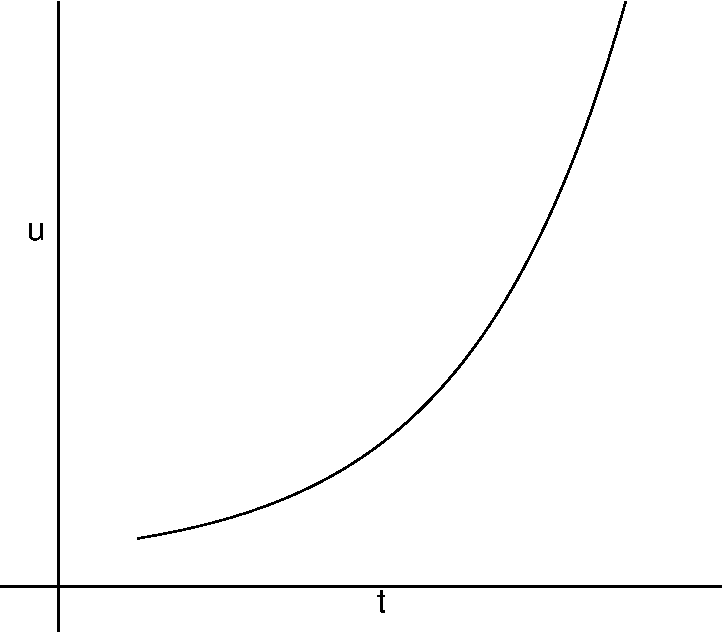
\includegraphics[width=0.5\textwidth]{exp_growth.pdf}
\caption{Exponential growth}
\label{expgrowth}
\end{figure}

\newpage

\item[C.] \textbf{Differential equation}


Population is $u(t)$. What is the \textbf{rate of change} of the
population?

In a time interval $\delta t$:
\begin{itemize}
\item A proportion $a \delta t$ of population produce
children.

\item A proportion $b \delta t$ of population die.

\item A proportion $c \delta t$ of population emigrate to Mars.
\end{itemize}

So,
\begin{align*}
& u(t + \delta t)  =  u(t) + (a-b-c)u(t) \delta t  \\
\Longrightarrow & \dfrac{u(t+\delta t) - u(t)}{\delta t} =
\lambda u(t),
\end{align*}
where $\lambda = a - b - c$.

\end{description}

Let $\delta t \to 0$ (see analysis course).

Then
  \begin{align*}
    \dfrac{du(t)}{dt} & =  \lambda u(t)  \\
    u(t_{0}) & = u_{0}
  \end{align*}

A differential equation like this, describing population growth, was used by Thomas Malthus, early 19th century.

\subsection*{Parameter estimation}

The UN estimates that the population grows by $1.14\%$ per year.

Let $t$ be time in years.

We separate the variables in our differential equation, then integrate (details later, when we study differential equations).
  \begin{align*}
    \dfrac{du}{dt} & = \lambda u  \\
    \implies \int \dfrac{1}{u} \, du & = \int \lambda \, dt  \\
    \implies u(t) & = u_{0} e^{\lambda(t-t_{0})}
  \end{align*}

We are interested in the change over one year, so let $t_{0}=t$, so $u_{0}=u(t)$, and consider
  \begin{align*}
    u(t + 1) & = u(t)e^{\lambda(t + 1 - t)}  \\
    & = u(t)e^{\lambda}  \\
    \implies \frac{u(t+1)-u(t)}{u(t)} & = \frac{u(t)e^{\lambda} - u(t)}{u(t)}  \\
    & = e^{\lambda} - 1.
  \end{align*}
This is the proportional increase in population over one year, so the UN estimate tells us that
  \begin{align*}
    e^{\lambda} - 1 & = 0.0114 \qquad (1.14\% \text{ growth})  \\
    \implies \lambda & = \ln (1+ 0.0114) \approx 0.01133551
  \end{align*}

Hence
\[
 u(t) = u_{0} e^{0.01133551(t-t_{0})}
\]
\end{example}

\subsection*{Application}

How long would it take for the population to double?

Pros:
\begin{itemize}[topsep=0pt]
\item Model easy to solve
\item Gives testable predictions
\end{itemize}

Cons:
\begin{itemize}[topsep=0pt]
 \item Unrealistic -- does not include effects of resource depletion, over-crowding, medical advances, agricultural advances, etc.
\end{itemize}

% I've cut this next paragraph because (a) I didn't like it; (b) the third point is vague/meaningless; (c) the fourth point makes the whole thing self-defeating (as, indeed, this kind of maths is).
%Generally
%\begin{itemize}[topsep=0pt]
% \item Use of differential equations started with Newton.
% \item Differential equations arise in many fields, including the sciences, engineering, economics, astronomy, etc.
% \item Very powerful approach.
% \item Most realistic models need a computer to solve.
%\end{itemize}

% This bit now unfortunately spills onto another page.
% (This sort of thing probably goes to pot when typesetting in large print anyway.)
To construct more realistic models, we will need to be able to
  \begin{itemize}[topsep=0pt]
    \item work with more than one independent variable;
    \item construct and solve more complex differential equations;
    \item evaluate more complex integrals.
  \end{itemize}




\newpage
\section{Integration}

Recall: There are two different types of integral.  Suppose we have a function $f$.
  \begin{enumerate}
    \item The \emph{indefinite integral} of $f$ is a function $F$ such that
      \[
        \frac{dF}{dx} = f(x).
      \]
    We write
      \[
        F = \int f \, dx.
      \]
    This defines integration as the inverse of differentiation (antidifferentiation). $F$ is called the \emph{antiderivative} of $f$.
    \item The \emph{definite integral} is defined as the \emph{net signed area} between $f$ and the horizontal axis between $a$ and $b$. It is written
      \[
        \int_{a}^{b} f(x) \, dx.
      \]
  \end{enumerate}

You are probably used to using indefinite integrals to evaluate definite integrals, e.g.
  \begin{align*}
    \int_{0}^{\pi/2} \sin(x) dx &= [-\cos(x)]_{0}^{\pi/2} \\
    &= 0 - (-1) \\
    &= 1.
  \end{align*}
But why are we allowed to combine definite and indefinite integrals in this way?


\subsection{Fundamental Theorem of Calculus}

This theorem establishes the astonishing connection between indefinite and definite integrals.

\begin{theorem}

Let $f$ be a continuous function on $u \in [a,b]$.

\emph{Part A.}

The function $f$ has an antiderivative $g$ given by
\[
 g(x) = \int_{a}^{x} f(u) du
\]
(signed area between $a$ and $x$, definite integral).

\emph{Part B.}

Given any antiderivative $h$ of $f$,
\begin{eqnarray*}
 \int_{a}^{b} f(u) \, du &=& h(b) - h(a) \\
 &=& g(b) - g(a)\\
&=& \int f(x)dx \Big|_{x=b} - \int f(x)dx \Big|_{x=a}
 \end{eqnarray*}

 \end{theorem}

We don't have the formal mathematics required to prove this rigorously, and won't have until Semester 2 of Analysis 1.  Isaac Newton didn't have that formal mathematics yet either, so we (roughly) followed the method of justification he used in 1669.
% I could possibly add more detail about what he did - which I think was just a special case - after the "proof".


\begin{proof}[Justification of Part A]

We wish to differentiate
\[
 g(x) = \int_{a}^{x} f(u) \, du.
\]

Suppose $x$ changes by a small increment $\Delta x$.  The corresponding change in $g$ is $g(x + \Delta x) - g(x)$, so the average rate of change from $x$ to $x + \Delta x$ is
  \[
	  \frac{\Delta g}{\Delta x} = \frac{g(x + \Delta x) - g(x)}{\Delta x}.
	\]

As $\Delta x \rightarrow 0$, this approaches the derivative $\dfrac{dg}{dx}$.

Now, consider the diagram in figure (\ref{FTC_Proof}).

  \begin{figure}[H]
    \centering
    \def\svgwidth{0.8\columnwidth}
    \input{figures/latex/FTC_Proof.pdf_tex}
    \caption{The area $g(x+\Delta x) = \text{area $A$} + \text{area $\Delta A$}$}
    \label{FTC_Proof}
  \end{figure}
By definition of the definite integral defining $g$,
\[
g(x+\Delta x) = \text{area $A$} + \text{area $\Delta A$} = g(x) + \text{area $\Delta A$}.
\]

There is a point $\hat{x}$ with $x \leq \hat{x} \leq x + \Delta x$ such that $\Delta A = f(\hat{x})\Delta x$, as shown in figure (\ref{FTC_Proof}).  So
\begin{align*}
 g(x+\Delta x) - g(x) &= \text{area $\Delta A$} \\
 &= f(\hat{x})\Delta x
 \end{align*}

 Hence
 \[
  \dfrac{g(x+\Delta x) - g(x)}{\Delta x} = f(\hat{x})
 \]

 As $\Delta x \to 0$, $\hat{x} \to x$ (since it gets sandwiched between $x$ and $x + \Delta x$), so \(f(\hat{x}) \to f(x)\) and
 \[
  \dfrac{dg}{dx} = f(x)
 \]

Hence $g$ is an antiderivative for $f$.

(see Analysis 1 Semester 2 for a rigorous proof).

\end{proof}

Note that this result allows us to differentiate certain functions defined in terms of integrals.  Explicitly, the statement ``$g$ is an antiderivative for $f$'' means that
  \[
    \frac{dg}{dx} = \frac{d}{dx}\left(\int_{a}^{x} f(u) \, du\right) = f(x).
  \]
Notice also that the derivative of $g$ does not depend on the lower limit of the integral, $a$.  If we were to evaluate the integral and write an explicit expression for $g$ (assuming that this is possible), this constant $a$ would only contribute a constant term to that expression; the derivative of that constant term would therefore be $0$.



\begin{proof}[Justification of Part B]

Let $h$ be an antiderivative of $f$.

So
\begin{eqnarray*}
 && \dfrac{dh}{dx} = f = \dfrac{dg}{dx}\\
% && F(x) = \int_{0}^{x} f(u)du \\
 &\Longrightarrow& \dfrac{dh}{dx} - \dfrac{dg}{dx} = 0\\
 &\Longrightarrow& \dfrac{d}{dx}(h-g) = 0\\
 && \text{by linearity of derivative}\\
 &\Longrightarrow& h-g=c, \quad \text{constant}.
\end{eqnarray*}

Hence
\[
 h=g+c.
\]

Now
\begin{eqnarray*}
 \int_{a}^{b} f(x)dx &=& \int_{a}^{x} f(u)du \Big|_{x=b}\\
 &=& g(x)\Big|_{x=b} = g(b)
\end{eqnarray*}
\begin{eqnarray*}
 \int_{a}^{a} f(x)dx &=& g(a)=0,
\end{eqnarray*}
so
\begin{eqnarray*}
 \int_{a}^{b} f(x)dx &=&  g(b) - g(a)\\
 &=& (g(b)+c) - (g(a)+c)\\
 &=& h(b) - h(a)
\end{eqnarray*}

\end{proof}

% I'm not convinced that this corollary is useful or enlightening.
% I think the point is that it's common-ish for functions to be defined as integrals, and these functions are therefore easy to differentiate.
\begin{corollary}
 \[
  \dfrac{d}{dx} \int_{a(x)}^{b(x)} f(u)du = f(b) \dfrac{db}{dx} - f(a) \dfrac{da}{dx}
 \]
\end{corollary}

\begin{proof}
 Let $g(x)$ be an antiderivative of $f(x)$, so
 \[
  \dfrac{dg}{dx} = f(x)
 \]

 Then by Fundamental Theorem of Calculus,
 \[
  \int_{a(x)}^{b(x)} f(u)du = g(b(x))-g(a(x))
 \]

 \begin{eqnarray*}
  \Longrightarrow \quad \dfrac{d}{dx} \int_{a(x)}^{b(x)} f(u)du &=&
  \dfrac{dg}{db} \dfrac{db}{dx} - \dfrac{dg}{da} \dfrac{da}{dx}\\
  && \text{(chain rule)}\\ % This kind of typesetting is hideous.
  &=& f(b) \dfrac{db}{dx} - f(a) \dfrac{da}{dx}
 \end{eqnarray*}
\end{proof}



\subsection{Hyperbolic functions}

Hyperbolic functions are a type of function related to trigonometric functions.  We will use them to help us integrate various types of functions, using a technique called \emph{integration by substitution}, which we'll meet in the next section.

\begin{eqnarray*}
 && \cosh (x) = \dfrac{1}{2} (e^{x}+e^{-x})\\
 && \sinh (x) = \dfrac{1}{2} (e^{x}-e^{-x})\\
 && \tanh (x) = \dfrac{\sinh (x)}{\cosh (x)} = \dfrac{e^{x}-e^{-x}}{e^{x}+e^{-x}}
\end{eqnarray*}


\subsubsection*{Sketches}

What do $\cosh$ and $\sinh$ look like?

$\cosh(0)=1$

As $x \to \infty$, $\cosh(x) \to \infty$.

As $x \to -\infty$, $\cosh(x) \to \infty$.

$\cosh (x)>0$ $\forall x$.

\begin{figure}[H]
\centering
 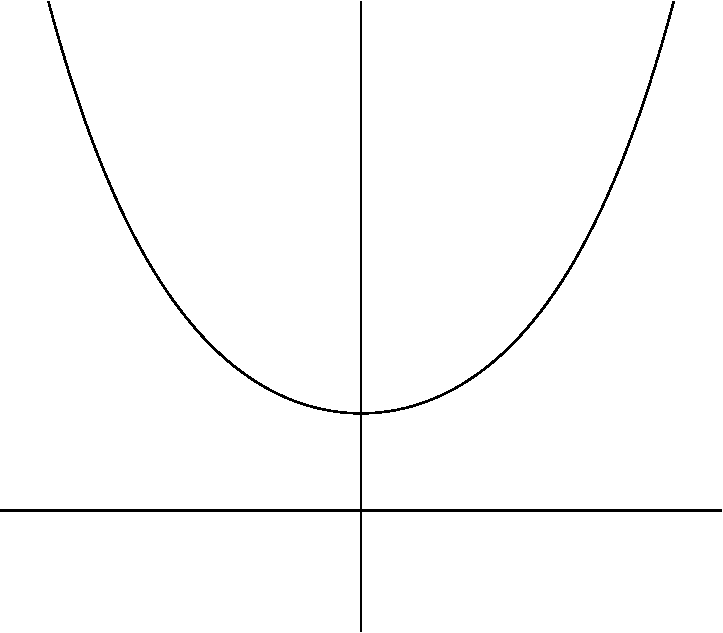
\includegraphics[width=0.6\textwidth]{cosh.pdf}
%\captionsetup{labelformat=empty}
\caption{$\cosh(x)$}
\end{figure}

Hanging chains (e.g. those in suspension bridges) have $\cosh$ shape, called a "catenary".

Soap bubbles between wands have a surface derived from the $\cosh$ shape.

$\sinh(0)=0$

As $x \to \infty$, $\sinh(x) \to \infty$.

As $x \to -\infty$, $\sinh(x) \to -\infty$.

\begin{figure}[H]
\centering
 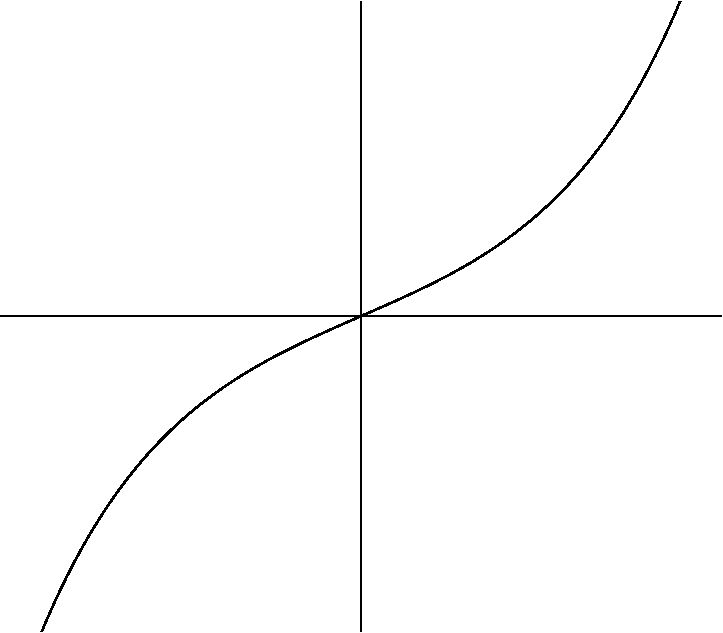
\includegraphics[width=0.6\textwidth]{sinh.pdf}
%\captionsetup{labelformat=empty}
\caption{$\sinh(x)$}
\end{figure}

$\tanh(0)=0$

As $x \to \infty$, $\tanh(x) \to 1$.

As $x \to -\infty$, $\tanh(x) \to -1$.

\begin{figure}[H]
\centering
 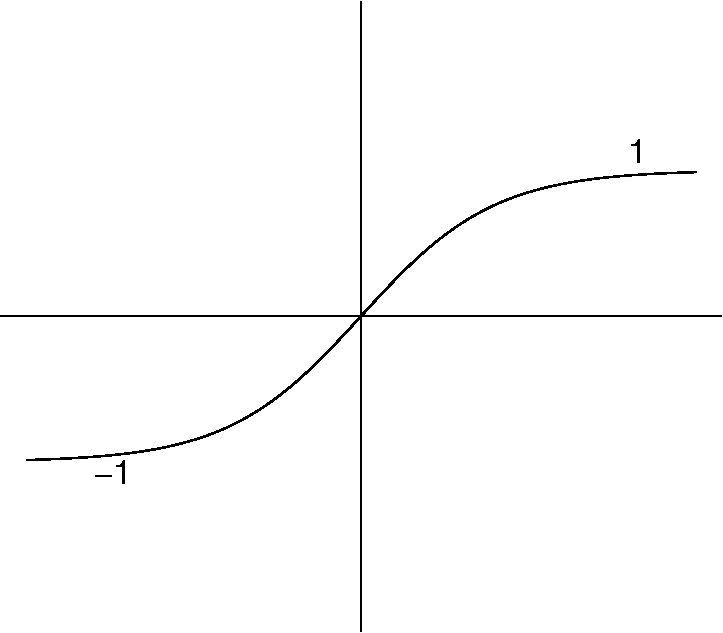
\includegraphics[width=0.6\textwidth]{tanh.pdf}
%\captionsetup{labelformat=empty}
\caption{$\tanh(x)$}
\end{figure}

\subsubsection*{Hyperbolic identities}

Hyperbolic functions satisfy identities similar to trigonometric identities.

\begin{examples}
  \quad
  \begin{enumerate}
		\item \(\cosh^{2}(x) - \sinh^{2}(x) = 1\) because
\begin{eqnarray*}
 \cosh^{2}(x) - \sinh^{2}(x)
 &=& \left(\dfrac{e^{x}+e^{-x}}{2}\right)^2
 - \left(\dfrac{e^{x}-e^{-x}}{2}\right)^2 \\
 &=& \dfrac{1}{4} \left(e^{2x} + 2 + e^{-2x}\right)
 - \dfrac{1}{4} \left(e^{2x} - 2 + e^{-2x}\right) \\
 &=& \dfrac{1}{2} + \dfrac{1}{2} = 1.
\end{eqnarray*}

Compare this with the trigonometric identity
\[
 \cos^{2}(x) + \sin^{2}(x) = 1.
\]
    \item \(1 - \tanh^2(x) = \sech^2(x).\)  Using \(\cosh^2(x) - \sinh^2(x) = 1\) and dividing through by \(\cosh^2(x)\) gives
		\[
		  \frac{\cosh^2(x)}{\cosh^2(x)} - \frac{\sinh^2(x)}{\cosh^2(x)} = \frac{1}{\cosh^2(x)},
		\]
		i.e. \(1 - \tanh^2(x) = \sech^2(x).\)
		
		Compare this with the trigonometric identity 
		  \[
			  1 + \tan^2(x) = \sec^2(x).
			\]
		\item The hyperbolic addition formula for \(\sinh\) is
		  \[
			  \sinh(x + y) = \sinh(x)\cosh(y) + \cosh(x)\cosh(y).
			\]
		The corresponding trigonometric identity is
		  \[
			  \sin(x + y) = \sin(x)\cos(y) + \cos(x)\cos(y).
			\]
		(See Exercise Sheet 1.)
		\item The hyperbolic addition formula for \(\cosh\) is
		  \[
			  \cosh(x + y) = \cosh(x)\cosh(y) + \sinh(x)\sinh(y).
			\]
		The corresponding trigonometric identity is
		  \[
			  \cos(x + y) = \cos(x)\cos(y) - \sin(x)\sin(y).
			\]
	\end{enumerate}
\end{examples}	

% I'm not sure that this Osborn's Rule stuff is strictly necessary, although the part about complex numbers is enlightening.

	In fact, \emph{Osborn's Rule} states that any trigonometric identity can be converted into a hyperbolic identity by
	  \begin{itemize}
			\item replacing trigonometric functions with their hyperbolic counterparts,
			\item swapping the sign of any product of two \(\sinh\)s.
		\end{itemize}
	Note: be careful with the second step, e.g.
	  \[
		  \tanh(x) = \frac{\sinh(x)}{\cosh(x)},
		\]
	so \(\tan^2(x)\) becomes \(-\tanh^2(x)\) (see Example 2).
	
	This arises because hyperbolic and trigonometric functions are related as follows:
	  \begin{align*}
		  \cosh(ix) & = \cos(x),  \\
			\cosh(x) & = \cos(ix),  \\
			\sinh(ix) & = i\sin(x),  \\
			\sinh(x) & = -i\sin(ix),
		\end{align*}
	where \(i^2 = -1\).
	
	This comes from Euler's relation:
	  \[
		  e^{i\theta} = \cos(\theta) + i\sin(\theta).
		\]
		
		
\subsubsection*{Geometric interpretation}

In trigonometric expressions such as \(\sin(\theta)\), \(\cos(\theta)\), etc., \(\theta\) can be interpreted as an angle.  Similarly, in \(\sinh(t)\) and \(\cosh(t)\), \(t\) can be interpreted as an area.

Since \(\cosh^2(t) - \sinh^2(t) = 1\), for any \(t\), the point \((x, y) = (\cosh(t), \sinh(t))\) lies on the curve \(x^2 - y^2 = 1\).  Then \(t\) corresponds to twice the area bounded by this curve, the \(x\)-axis, and the line from the origin to the point \((\cosh(t), \sinh(t))\), as shown in figure (\ref{inversehyperbolicarea}).

  \begin{figure}[H]
    \centering
    \def\svgwidth{0.8\columnwidth}
%    \def\svgwidth{0.3\columnwidth}
    \input{figures/latex/Inverse_Hyperbolic_Area.pdf_tex}
    \caption{$t$ corresponds to twice the shaded area}
    \label{inversehyperbolicarea}
  \end{figure}

Because of this, the inverse hyperbolic functions are denoted \(\arsinh\), \(\arcosh\), etc. -- ``ar'' is an abbreviation of ``area''.


\subsubsection*{Differentiating hyperbolic functions}

Since hyperbolic functions are defined in terms of the exponential function, they are straightforward to differentiate.

\begin{align*}
  \frac{d}{dx}\sinh(x) & = \frac{d}{dx}\left(\frac{e^x - e^{-x}}{2}\right)  \\
                       & = \frac{e^x + e^{-x}}{2}  \\
                       & = \cosh(x)
\end{align*}

Similarly,
  \[
    \frac{d}{dx}\cosh(x) = \sinh(x),
  \]
  \[
    \frac{d}{dx}\tanh{x} = \frac{1}{\cosh^2(x)} = \sech^2(x).
  \]




\subsection{Integrating functions involving square roots}  \label{sect:sqrts}

Integrals involving functions with square roots often arise in mechanics.  In this section, we will investigate methods for integrating them using trigonometric and hyperbolic substitutions.

Recall that integration by substitution is a technique for evaluating integrals involving composite functions, using the formula
  \[
    \int f(g(x)) \dfrac{dg}{dx}dx = F(g(x)) + c,
  \]
derived from the chain rule for differentiation. (For a more detailed reminder of integration by substitution, see the additional notes on the course Moodle page.)


\begin{example}

Evaluate the integral
  \[
	  \int \sqrt{a^2 - x^2} \, dx,
	\]
where \(\left|x\right| < a\).

The integrand is a semicircle with radius \(a\).  To inform which choice of substitution to use, consider figure (\ref{semicircleintegralindefinite}).  The coordinates of any point \((x, \sqrt{a^2 - x^2})\) on the curve can be expressed in terms of \(\theta\), the angle between the \(y\)-axis and the line segment from the origin to that point, using trigonometric functions.

  \begin{figure}[H]
    \centering
    \def\svgwidth{0.55\columnwidth}
    \input{figures/latex/semicircleintegralindefinite.pdf_tex}
    \caption{Finding a substitution to integrate the curve $\sqrt{a^2 - x^2}$}
    \label{semicircleintegralindefinite}
  \end{figure}
	

From the right-angled triangle in figure (\ref{semicircleintegralindefinite}), we see that
  \[
    x  =  a \sin{\theta}.
  \]
We will use this for our substitution.  Then $\theta=\arcsin \left(\dfrac{x}{a}\right)$,\quad $\dfrac{dx}{d \theta} = a \cos(\theta)$, and
  \[
	  \sqrt{a^2 - x^2} = \sqrt{a^2 - a^2\sin^2(\theta)} = \sqrt{a^2\cos^2(\theta)} = a\cos(\theta),
	\]
using \(1 - \sin^2(\theta) = \cos^2(\theta)\); alternatively, one can deduce this from the right-angled triangle in figure (\ref{semicircleintegralindefinite}).

%% Thus the integral is
%%   \begin{align*}
%%     \int \sqrt{a^2 - x^2} \, dx & = \int a\cos(\theta) \times a\cos(\theta) \, d\theta \\
%%     & = \int a^2 \cos^2(\theta) \, d\theta \\
%%     & = \int \frac{a^2}{2}\left(1+\cos(2\theta)\right) \, d\theta \\
%%     & = \frac{a^2}{2} \theta + \frac{a^2}{4} \sin(2\theta) + c \\
%%     & = \frac{a^2}{2} \arcsin \left(\frac{x}{a}\right)+\frac{a^2}{4} \sin \left(2 \arcsin\left(\frac{x}{a}\right)\right) +c.\\
%%   \end{align*}

%% The second term can be simplified further: using the trigonometric identities
%%   \begin{align*}
%% 	  \sin (2\theta) & = 2 \sin (\theta) \cos (\theta), \text{ and}   \\
%% 		\cos (\theta) & = \sqrt{1-\sin^{2}(\theta)},
%% 	\end{align*}
%% we have
%%   \begin{align*}
%% 	  \sin \left(2 \arcsin\left(\frac{x}{a}\right)\right) & = 2 \sin \left(\arcsin\left(\frac{x}{a}\right)\right)\cos \left(\arcsin\left(\frac{x}{a}\right)\right)  \\
%% 		& = 2\dfrac{x}{a} \left[1 - \sin^2 \left(\arcsin\left(\frac{x}{a}\right)\right) \right]^{1/2}  \\
%% 		& = \dfrac{2x}{a} \sqrt{1-\dfrac{x^{2}}{a^{2}}}.
%% 	\end{align*}
%% Thus
%%   \begin{align*}
%%     \int \sqrt{a^2 - x^2} \, dx & = \frac{a^2}{2} \arcsin \left(\frac{x}{a}\right)+\frac{a^2}{4} \sin \left(2 \arcsin\left(\frac{x}{a}\right)\right) +c.\\
%% 		& = \frac{a^2}{2} \arcsin \left(\frac{x}{a}\right) + \frac{ax}{2} \sqrt{1-\dfrac{x^2}{a^2}} + c  \\
%% 		& = \frac{a^2}{2} \arcsin \left(\frac{x}{a}\right) + \frac{x}{2} \sqrt{a^2 - x^2} + c.
%%   \end{align*}
	
%% For a geometric interpretation of this answer, consider the definite integral
%%   \begin{equation}  \label{semicircledefiniteexpression}
%% 	  \int_0^b \sqrt{a^2 - x^2} \, dx = \frac{a^2}{2}\arcsin\left(\frac{b}{a}\right) + \frac{b}{2} \sqrt{a^2 - b^2},
%% 	\end{equation}
%% where \(0 < b < a\).  This definite integral is the area shown in figure (\ref{semicircleintegraldefinite}), divided into two regions, \(R\) and \(S\).

%%   \begin{figure}[H]
%%     \centering
%%     \def\svgwidth{0.4\columnwidth}
%%     \input{figures/latex/semicircleintegraldefinite.pdf_tex}
%%     \caption{Definite integral of the curve $\sqrt{a^2 - x^2}$}
%%     \label{semicircleintegraldefinite}
%%   \end{figure}
	
%% The region \(R\) is a sector of a circle of radius \(a\) with angle \(\arcsin\left(\dfrac{b}{a}\right)\), and therefore has area
%%   \[
%% 	  \frac{\pi a^2}{2\pi}\arcsin\left(\frac{b}{a}\right) = \frac{a^2}{2}\arcsin\left(\frac{b}{a}\right),
%% 	\]
%% the first term in the expression for the definite integral (\ref{semicircledefiniteexpression}).

%% The region \(S\) is a triangle with base length \(b\) and height \(\sqrt{a^2 - b^2}\), and therefore has area
%%   \[
%% 	  \frac{b}{2} \sqrt{a^2 - b^2},
%% 	\]
%% the second term in the expression for the definite integral (\ref{semicircledefiniteexpression}).
%% \end{example}

%% There are a total of six similar cases (including this one) of integrals involving square roots:
%%   \begin{enumerate}
%%     \item $\sqrt{a^2 - x^2}$ \qquad ($\left|x\right| < a$)
%%     \item $\dfrac{1}{\sqrt{a^2 - x^2}}$ \qquad ($\left|x\right| < a$)
%%     \item $\dfrac{1}{\sqrt{a^2 + x^2}}$
%%     \item $\sqrt{a^2 + x^2}$
%%     \item $\dfrac{1}{\sqrt{x^2 - a^2}}$ \qquad ($\left|x\right| > a$)
%%     \item $\sqrt{x^2-a^2}$\qquad ($\left|x\right| > a$)
%%   \end{enumerate}

%% \begin{description}
%% \item[Case 2.]  This integrand includes the same square root expression as Case 1, so we use the same substitution,
%%   \[
%%     x  =  a \sin{\theta}.
%%   \]
%% With this substitution, $\theta=\arcsin \left(\dfrac{x}{a}\right)$ and $\dfrac{dx}{d \theta} = a \cos(\theta)$.

%%   \begin{align*}
%%     \int \dfrac{1}{\sqrt{a^2-x^2}} \, dx & = \int \dfrac{a \cos (\theta)}{\sqrt{a^2 - a^2\sin^2(\theta)}} \, d\theta  \\
%% 		& = \int \dfrac{a \cos (\theta)}{a \cos(\theta)} \, d\theta  \\
%% 		& = \int  d\theta \\
%% 		& = \theta + c \\
%% 		& = \arcsin\left(\dfrac{x}{a}\right) + c.
%% \end{align*}

%% \item[Case 3.] In Cases 1 and 2, we simplified the square root using the trigonometric identity
%%   \[
%% 	  1 - \sin^2(\theta) = \cos^2(\theta).
%% 	\]
%% In this case, we will use the hyperbolic identity
%%   \[
%% 	  1 + \sinh^2(\theta) = \cosh^2(\theta)
%% 	\]
%% in a similar way.  To do this, we use the substitution $x=a \sinh(\theta)$,  so
%%   \[
%%     \theta = \arcsinh \left(\dfrac{x}{a}\right), \qquad \dfrac{dx}{d\theta} = a \cosh(\theta).
%%   \]

%% \begin{eqnarray*}
%%  && \int \dfrac{dx}{\sqrt{a^2+x^2}} \\
%%  &=& \int \dfrac{a \cosh (\theta) d\theta}{\sqrt{a^2+a^2 \sinh^2(\theta)}} \\
%%  &=& \int \dfrac{a \cosh (\theta)}{a \cosh(\theta)}  d\theta \\
%% &=& \theta + c\\
%% &=& \arcsinh \left(\dfrac{x}{a}\right) + c\\
%%  \end{eqnarray*}

%% Recall from Exercise Sheet 1, question 4(a), that
%% \[
%%  \arcsinh (u) = \ln (u+\sqrt{u^2+1}),
%% \]
%% so
%%   \[
%%     \int \dfrac{dx}{\sqrt{a^2+x^2}} = \ln (x+\sqrt{x^2+a^2}) + c.
%%   \]

%% \item[Case 4, 5 and 6.] See Exercise Sheet 2.

%% \end{description}



%% \subsection{Integrating rational functions}

%% In this section, we will investigate methods for integrating rational functions.  A rational function is a function of the form
%% \[
%%  f(x) = \dfrac{a+bx+cx^{2} + \ldots + dx^{n}}{p + qx + rx^{2} + \ldots + sx^{m}}.
%% \]
%% They can be used to approximate many other functions.

%% \subsubsection*{Numerator $1$, denominator linear}

%% \begin{eqnarray*}
%%  f(x) &=& \dfrac{1}{ax+b}\\
%%  &=& \dfrac{1}{a} \times \dfrac{a}{ax+b}\\
%%  &=& \dfrac{1}{a} \dfrac{1}{g(x)} \dfrac{dg}{dx}\\
%%  \text{where } g(x) &=& ax+b
%% \end{eqnarray*}

%% So
%% \[
%%  \int f(x) dx = \dfrac{1}{a} \ln \left|ax+b\right| + c
%% \]

%% \subsubsection*{Numerator $1$, denominator quadratic}

%% \[
%%  f(x) = \dfrac{1}{ax^{2}+bx+c}
%% \]

%% We first consider two simpler cases, then show how the general case can be reduced to one of these.

%% \begin{examplesnumbered} \label{ex:quadraticdenominators}
%%  \quad
%%  \begin{enumerate}
%%   \item $f(x) = \dfrac{1}{a^{2} + x^{2}}$

%%          Substitution: let $x = a \tan(u)$, so that $u = \arctan \left(\dfrac{x}{a}\right)$.
%% 				% This could do with more explanation about why I'm using that substitution.
				
%% 				Then
%% 				  \[
%% 					  \frac{dx}{du} = a\sec^2(u),
%% 					\]
%% 				so
%% 				  \begin{align*}
%% 					  \int \frac{1}{a^2 + x^2} \, dx & = \int \frac{1}{a^2 + a^2\tan^2(u)} \times a\sec^2(u) \, du  \\
%% 						& = \int \frac{a\sec^2(u)}{a^2(1 + \tan^2(u))} \, du  \\
%% 						& = \int \frac{a\sec^2(u)}{a^2\sec^2(u)} \, du  \\
%% 						& = \int \frac{1}{a} \, du  \\
%% 						& = \frac{u}{a} + c  \\
%% 						& = \frac{1}{a}\arctan\left(\frac{x}{a}\right) + c.
%% 					\end{align*}

%%     \item $f(x) = \dfrac{1}{a^{2}-x^{2}} = -\dfrac{1}{x^{2}-a^{2}}$
		
%% 		In this case, we have several options:
%% 		  \begin{itemize}
%% 				\item Use partial fractions:
%% 				  \begin{align*}
%% 					  f(x) & = \frac{1}{(a + x)(a - x)}  \\
%% 						& = \frac{1}{2a}\left(\frac{1}{a + x} + \frac{1}{a - x}\right).
%% 					\end{align*}
%% 				\item If \(|x| < a\), use \(x = a\tanh(u)\).  Then \(a^2 - x^2 = a^2(1 - \tanh^2(u)) = a^2\sech^2(u)\).
%% 				\item If \(|x| > a\), use \(x = a\coth(u)\), so \(a^2 - x^2 = a^2(1 - \coth^2(u)) = -a^2\cosech^2(u)\).
%% 			\end{itemize}
%% 		We will not cover the details of the substitutions here, since they are so similar to the \(\tan\) substitution in Case 1.
%%  \end{enumerate}

%% \end{examplesnumbered}


%% \subsubsection*{General quadratic denominator}

%% Given an integral with a general quadratic denominator,
%%     \begin{equation}  \label{eq:genquadraticdenom}
%%       \int \dfrac{dx}{ax^{2} + bx + c},
%%     \end{equation}
%% we perform the following steps:
%%   \begin{itemize}
%% 		\item Complete the square in the denominator.
%% 		\item Use a substitution to transform this into
%% 		  \[
%% 			  \int \frac{p}{u^2 \pm q^2} \, du,
%% 			\]
%% 		with \(p\) and \(q\) constant.
%% 		\item If \(q = 0\), this can be integrated directly.
%% 		\item Otherwise, integrate using the method from Case 1 or Case 2 from Examples~\ref{ex:quadraticdenominators}.
%% 	\end{itemize}
	
%% 	\begin{examplenumbered} \label{ex:genquaddenom}
%% 	  Evaluate
%% 		  \[
%% 			  \int \frac{dx}{x^2 + 4x + 8} = \int \frac{dx}{(x + 2)^2 + 4}.
%% 			\]
%% 		We have completed the square in the denominator.  Now let \(u = x + 2\), so \(\dfrac{du}{dx} = 1\).  Then
%% 		  \begin{align*}
%% 			  \int \frac{dx}{(x + 2)^2 + 4} & = \int \frac{du}{u^2 + 2^2}  \\
%% 				& = \frac{1}{2}\arctan\left(\frac{u}{2}\right) + c  \\
%% 				& = \frac{1}{2}\arctan\left(\frac{x + 2}{2}\right) + c.
%% 			\end{align*}
%% 	\end{examplenumbered}
	
%% 	For completeness, there follows an argument for evaluating \ref{eq:genquadraticdenom} for general values of \(a\), \(b\) and \(c\). 	Since this is notationally fiddly, but not substantially more complicated than the previous example, this general argument will not be covered in the lectures.

%% The denominator is
%% \begin{eqnarray}
%%  ax^{2} + bx + c &=& a \left[x^{2}+ \left(\dfrac{b}{a}\right)x + \left(\dfrac{c}{a}\right)\right]\notag\\
%%  &=& a \left[\left(x+ \dfrac{b}{2a}\right)^{2} + \dfrac{c}{a}-\dfrac{b^{2}}{4a^{2}}\right]\notag\\
%%   &=& a \left[\left(x+ \dfrac{b}{2a}\right)^{2} + \dfrac{4ac-b^{2}}{4a^{2}}\right]\label{eq4.5}.
%% \end{eqnarray}

%% To simplify the notation, write $\Delta=4ac-b^{2}$, which is a constant.  We make the substitution $u=x+\dfrac{b}{2a}$, so $\dfrac{du}{dx}=1$.

%% Then, from \eqref{eq4.5},
%% \[
%%  ax^{2} + bx + c = a \left[u^{2}+ \dfrac{\Delta}{4a^{2}}\right]
%% \]
%% so
%% \[
%%  \int \dfrac{dx}{ax^{2}+bx+c} = \dfrac{1}{a} \int \dfrac{du}{u^{2} + \dfrac{\Delta}{4a^{2}}}
%% \]

%% If $\Delta>0$, use $\tan$ substitution for $\dfrac{1}{q^2 + u^{2}}$ with $q = \dfrac{\sqrt{\Delta}}{2a}$.

%% If $\Delta<0$, use partial fractions or a $\tanh$ or \(\coth\) substitution for $-\dfrac{1}{q^2 - u^{2}}$ with $q = \dfrac{\sqrt{-\Delta}}{2a}$.

%% If $\Delta=0$, the integral does not require a substitution.

%% \subsubsection*{General quadratic numerator and denominator}

%% Given an integral with a general quadratic numerator and denominator,
%% \[
%%  \int \dfrac{px^{2} + qx + r}{ax^{2} + bx + c} dx,
%% \]
%% we use a series of transformations to break this into expressions that we already know how to integrate.

%%   \begin{example}
%% 	  Evaluate
%% 		  \[
%% 			  \int \frac{2x^2 + 6x + 15}{x^2 + 4x + 8} \, dx.
%% 			\]
%% 		We write \(f(x)\) for the integrand.  First, we manipulate the integrand to remove the \(x^2\) term from the numerator:
%% 		  \begin{align*}
%% 			  f(x) & = \frac{2x^2 + 6x + 15}{x^2 + 4x + 8}  \\
%% 				& = \frac{2(x^2 + 4x + 8) - 2x - 1}{x^2 + 4x + 8}  \\
%% 				& = 2 - \frac{2x + 1}{x^2 + 4x + 8}.
%% 			\end{align*}
%% 		We cannot do the same to simplify the linear over quadratic term; however, this would be straightforward to integrate if the numerator was the derivative of the denominator.
		
%% 		Observe: \(\dfrac{d}{dx}(x^2 + 4x + 8) = 2x + 4\), so we write
%% 		  \begin{align*}
%% 			  f(x) & = 2 - \frac{2x + 4 - 3}{x^2 + 4x + 8}  \\
%% 				& = 2 - \frac{2x + 4}{x^2 + 4x + 8} + \frac{3}{(x + 2) + 4}.
%% 			\end{align*}
			
%% 	We have broken \(f(x)\) into three terms that we can integrate.  Notice that the third term is a multiple of the function from Example~\ref{ex:genquaddenom}.  We get
%% 	\[
%% 	  \int f(x) \, dx = 2x - \ln(x^2 + 4x + 8) + \frac{3}{2}\arctan\left(\frac{x + 2}{2}\right) + c.
%% 	\]			
%%   \end{example}
	
%% 	As before, the fully general case will not be covered in lectures, but is included here for completeness:
%% \begin{eqnarray*}
%% && \int \dfrac{px^{2} + qx + r}{ax^{2} + bx + c} dx \\
%%  &=& \int \dfrac{\dfrac{p}{a} (ax^{2} + bx + c)}{ax^{2} + bx + c}
%%  + \dfrac{qx + r - \left[\dfrac{pb}{a}x - \dfrac{pc}{a}\right]}{ax^{2} + bx + c} dx\\
%% &=& \dfrac{px}{a} + \int \dfrac{ex+f}{ax^{2}+bx+c} dx \\
%% &=& \dfrac{px}{a} + \int \dfrac{\dfrac{e}{2a} (2ax+b)}{ax^{2}+bx+c} + \dfrac{f-\left[\dfrac{be}{2a}\right]}{ax^{2}+bx+c} dx\\
%% &=& \dfrac{px}{a} + \dfrac{e}{2a} \ln \left|ax^{2}+bx+c\right| + \left(f-\dfrac{be}{2a}\right) \int \dfrac{dx}{ax^{2}+bx+1}.
%% \end{eqnarray*}



%% \subsection{Reciprocals of trigonometric functions}

%% The methods in the previous have uses beyond integrating rational functions.  Certain other integrals can be evaluated by making a careful choice of substitution that converts the integrand into a rational function.

%% In the following examples we look at substitution that does this for integrals involving trigonometric functions.  The substitution we will use is not at all obvious substitution -- it was described by Michael Spivak (author of one of the recommended books for Analysis 1) as ``the world's sneakiest substitution''.

%% \begin{example}
%% Evaluate $\displaystyle\int \dfrac{d \theta}{2+\sin(\theta)+\cos(\theta)}$.

%% We will use the substitution $t=\tan \left(\dfrac{\theta}{2}\right)$.  Consider the right-angled triangle


%% \begin{center}
%% 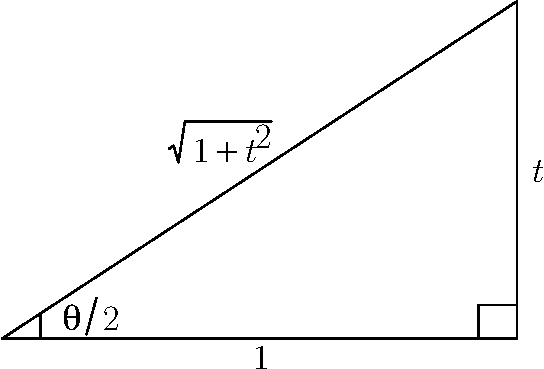
\includegraphics[width=0.45\textwidth]{triangle.pdf}
%% \end{center}

%% We have
%% \begin{eqnarray*}
%%  \sin \left(\frac{\theta}{2}\right) & = & \dfrac{t}{\sqrt{1+t^2}}, \\
%%  \cos \left(\frac{\theta}{2}\right) & = & \dfrac{1}{\sqrt{1+t^2}},
%% \end{eqnarray*}
%% so
%% \begin{eqnarray*}
%%  \sin(\theta) & = & 2 \sin \left(\frac{\theta}{2} \right) \cos
%% \left(\frac{\theta}{2} \right) \\
%% &= & \frac{2t}{(1+t^2)} \\
%%  \cos (\theta)& = & \cos^2 \left(\frac{\theta}{2} \right) -
%% \sin^2 \left(\frac{\theta}{2} \right) \\
%% & = &
%% \frac{(1-t^2)}{(1+t^2)}
%% \\
%%  \tan(\theta) & = & \frac{2 t}{(1-t^2)}
%% \end{eqnarray*}

%% Also
%% \begin{eqnarray*}
%% \frac{dt}{d \theta} & =& \frac{1}{2} \sec^2
%% \left(\frac{\theta}{2} \right) \\
%% & = & \frac{t^2+1}{2},
%% \end{eqnarray*}
%% so
%% \[
%%   \frac{d \theta}{dt}  =  \frac{2}{1+t^2}
%% \]

%% Observe that this substitution will convert any integral involving only $\sin$, $\cos$ and $\tan$, combined by addition, multiplication and division, into the integral of a rational function.  We now use it to evaluate the integral in our example.

%% Then
%% \begin{align*}
%% & \phantom{=} \int \frac{d \theta}{2+\sin(\theta)+\cos(\theta)}  \\
%% & = \int \frac{1}{2 + \left( \frac{2t}{1 + t^2} \right) + \left( \frac{1 - t^2}{1 + t^2} \right)} \times \frac{2}{1 + t^2} dt \\
%% & = \int\frac{2 dt}{t^2+2t+3} \\
%% & = \int \frac{2 dt}{(t+1)^2 + 2} \\
%% & = \sqrt{2} \arctan \left(\frac{1+t}{\sqrt{2}}\right) + c \\
%% & = \sqrt{2} \arctan \left(\frac{1+\tan(\theta/2)}{\sqrt{2}}\right) + c.
%% \end{align*}

%% \end{example}

%% % I have never done this example in the lectures and have omitted it for now.
%% % It would be nice on an exercise sheet, but there probably isn't space.

%% %\begin{example}
%%  %Suppose the radius $r$ of the orbit of a planet around its sun satisfies
%%  %\[
%%  %r=\dfrac{\ell}{1+k \cos(\theta)}, \qquad 0 \leq k \leq 1, \qquad l > 0.
%%  %\]
%% %
%%  %\begin{center}
%%   %\includegraphics[width=0.7\textwidth]{trig4.pdf}
%%  %\end{center}
%% %
%%  %What is the mean distance from the sun?  To find it we integrate the distance over all angles $\theta$, then divide by sum of all angles, $2\pi$.  We will be using the subtitution $t=\tan(\theta/2)$, so we must integrate from $\pi$ to $\pi$, since this substitution gives $\theta = 2\arctan(t)$, and
%%   %\[
%%     %- \frac{\pi}{2} < \arctan(t) < \frac{\pi}{2}
%%   %\]
%% %for all real numbers $t$.
%% %
%%  %\[
%%   %\overline{r} = \dfrac{1}{2\pi} \int_{-\pi}^{\pi} \dfrac{\ell}{1+k \cos(\theta)} d\theta
%%  %\]
%% %
%% %Let $t=\tan\left(\dfrac{\theta}{2}\right)$.  Then
%%   %\begin{align*}
%%     %\overline{r} & = \frac{1}{2\pi} \int_{\pi}^{\pi} \frac{l}{1 + k\cos(\theta)} \, d\theta  \\
%%     %& = \frac{l}{2\pi} \int_{-\infty}^{\infty} \frac{l}{1 + k\left( \frac{1 - t^2}{1 + t^2} \right)} \times \frac{2}{1 + t^2} \, dt  \\
%%     %& = \frac{l}{\pi} \int_{-\infty}^{\infty} \frac{1}{1 + t^2 + k - kt^2} \, dt  \\
%%     %& = \frac{l}{\pi} \int_{-\infty}^{\infty} \frac{1}{(1 - k)t^2 + (1 + k)} \, dt.
%%   %\end{align*}
%% %Now let $u = \sqrt{1 - k}t$, write $a = \sqrt{1 + k}$.  Then
%%   %\begin{align*}
%%     %\overline{r} & = \frac{l}{\pi} \int_{\pi}^{\pi} \frac{1}{u^2 + a^2} \times \frac{1}{\sqrt{1 - k}} \, du  \\
%%     %& = \frac{l}{\pi\sqrt{1 - k}} \left[ \frac{1}{a} \arctan\left( \frac{u}{a} \right) \right]_{-\infty}^{\infty}  \\
%%     %& = \frac{l}{\pi\sqrt{1 - k}\sqrt{1 + k}} \left[\frac{\pi}{2} - \left( - \frac{\pi}{2} \right)\right]  \\
%%     %& = \frac{l}{\sqrt{1 - k^2}}.
%%   %\end{align*}
%% %
%% %\end{example}




%% \subsection{Reduction formulae}

%% Recall that integration by parts is a technique for evaluating integrals involving products of functions using the formula
%%   \[
%%     \int u \frac{dv}{dx} \, dx   =   u v - \int v \frac{du}{dx} \, dx,
%%   \]
%% which is derived from the product rule for differentiation.  (For a more detailed reminder of integration by parts, see the additional notes on the course Moodle page.)

%% Sometimes complicated integrals can be reduced to simpler expressions by successive application of integration by parts, giving a type of formula called a \emph{reduction formula}.
%% % Not convinced by the wording of this last sentence.

%% \begin{examples}
%% \quad

%% \begin{enumerate}

%% \item $\displaystyle\int \left(\ln(x)\right)^n \, dx$,\quad $n=0,1,2,\dotsc$

%% Write
%%   \begin{align*}
%%     I_n & = \int \left(\ln(x)\right)^n \, dx  \\
%%     & = \int 1 \times (\ln(x))^ndx \\
%% 	\end{align*}
%% Let
%%   \[
%% 	  u = (\ln(x))^n, \quad \frac{dv}{dx} = 1,
%% 	\]
%% so
%%   \[
%% 	  \frac{du}{dx} = \frac{n(\ln(x))^{n - 1}}{x}, \quad v = x.
%% 	\]
%% Then, using integration by parts,
%% 	\begin{align*}
%%     I_n & = x (\ln(x))^n - \int x \frac{n (\ln(x))^{n-1}}{x} dx \\
%%     & = x (\ln(x))^n - n \int (\ln(x))^{n-1} dx \\
%%     I_n & = x (\ln(x))^n - n I_{n-1}
%%   \end{align*}
	
%% This formula allows us to evaluate \(I_n\) for a given value of \(n\) -- provided we also do so for all lower values of \(n\):
%%   \begin{align*}
%%     I_3 & = x[\ln(x)]^3 - 3 I_2, \\
%%     I_2 & = x [\ln(x)]^2 - 2 I_1, \\
%%     I_1 & = x \ln(x) - I_0, \\
%%     I_0 & = \int 1dx  =  x,
%% 	\end{align*}
%% so
%% 	\begin{align*}
%%     I_1 & = x\ln(x) - x, \\
%%     I_2 & = x[\ln(x)]^2 - 2 x \ln(x) + 2x, \\
%%     I_3 & = x[\ln(x)]^3 - 3 x [\ln(x)]^2 + 6 x \ln(x) - 6 x\ln(x) - 6x + C.
%%   \end{align*}

%% \item $I_n = \displaystyle\int \sin^n(x)dx$,\quad $n=0,1,2, \dotsc$
  
%% 	Write this as
%%   \[
%%     I_n = \int \sin(x) \sin^{n-1}(x) \, dx
%%   \]
%% Let 
%%   \[
%% 	  u = \sin^{n-1}(x), \quad \frac{dv}{dx} = \sin(x),
%% 	\]
%% so
%%   \[
%% 	  \frac{du}{dx} = (n - 1)\cos(x)\sin^{n-2}(x), \quad v = -\cos(x).
%% 	\]
%% Then, using integration by parts,
%%   \begin{align*}
%%     I_n & =  -\cos(x)\sin^{n-1}(x) + \int \cos(x) (n-1)\cos(x) \sin^{n-2}(x)dx  \\
%%     & = -\cos(x)\sin^{n-1}(x) + (n-1) \int \cos^2(x)\sin^{n-2}(x)dx
%%   \end{align*}
%% But $\cos^2(x) = 1 - \sin^2 (x)$
%%   \begin{align*}
%%     I_n & = -\cos(x)\sin^{n-1}(x) + (n-1)\int \sin^{n-2}(x)dx - (n-1)\int \sin^n (x)dx  \\
%%     & = -\cos(x)\sin^{n-1}(x) + (n-1) I_{n-2} - (n-1)I_n.
%% 	\end{align*}
	
%% 	Rearranging this gives
%% 	  \[
%% 		  I_n = \frac{1}{n} \left[-\cos(x)\sin^{n-1}(x)\right] + \frac{n-1}{n} I_{n-2}.
%% 		\]
  
%% 	We can use this calculate any \(I_n\).  For example, when \(n = 3\), we get
%% 	\begin{align*}
%%     I_3 & = \frac{1}{3} \left[-\cos(x)\sin^2(x)\right] + \frac{2}{3}I_1, \\
%%     I_1 & = \int \sin(x)dx  =  -\cos(x) + c, \\
%%     \therefore \quad I_3 & = -\frac{1}{3} \cos(x)\sin^2(x) - \frac{2}{3}\cos(x) + c.
%%   \end{align*}


%% % Removed this example -- it will be Exercise Sheet material only from now on.

%% %\item $\displaystyle\int \dfrac{dx}{(1+x^2)^{n}}$.
%% %
%% %\begin{eqnarray*}
%% %I_n &  = & \int \frac{dx}{(1+x^2)^n} \\
%% %I_1 &  = & \int \frac{dx}{1+x^2}  =  \int \frac{1 \times dx}{1+x^2} \\
%% %&  = & \frac{x}{1 + x^2} + \int \frac{2 x^2}{(1+x^2)^2}dx \\
%% %I_1 &  = & \frac{x}{1 + x^2} + 2 \int \frac{x^2 + 1 - 1}{(1 +
%% %x^2)^2} dx \\
%% %I_1 &  =  &\frac{x}{1 + x^2} + 2 \int \frac{dx}{(1 +
%% %x^2)}  - 2 \int \frac{dx}{(1 + x^2)^2} \\
%% %I_1 &  = & \frac{x}{1+x^2} + 2 I_1 - 2I_2 \\
%% %\therefore \qquad I_2 &  = & \frac{1}{2}
%% %\left[\dfrac{x}{1+x^2}\right] + \dfrac{I_1}{2} \\
%% %I_1 &  = & \arctan(x) + c
%% %\end{eqnarray*}
%% %
%% %Now find $I_{n+1}$ given $I_{n}$ (See Exercie Sheet 3).
%% % Check which worksheet it is once the worksheets are ready!

%% \end{enumerate}
%% \end{examples}


%% \subsection{Arc length and surface areas of revolution}


%% \subsubsection*{Arc length} 
%% We often need to know the length of a curve between two points,
%% e.g.\ what is the length of the ropes holding Clifton suspension bridge
%% (see Exercise Sheet 3).

%% \textbf{Idea. } Given a curve $y=y(x)$

%%   \begin{figure}[H]
%%     \centering
%%    % \def\svgwidth{0.4\columnwidth}
%%     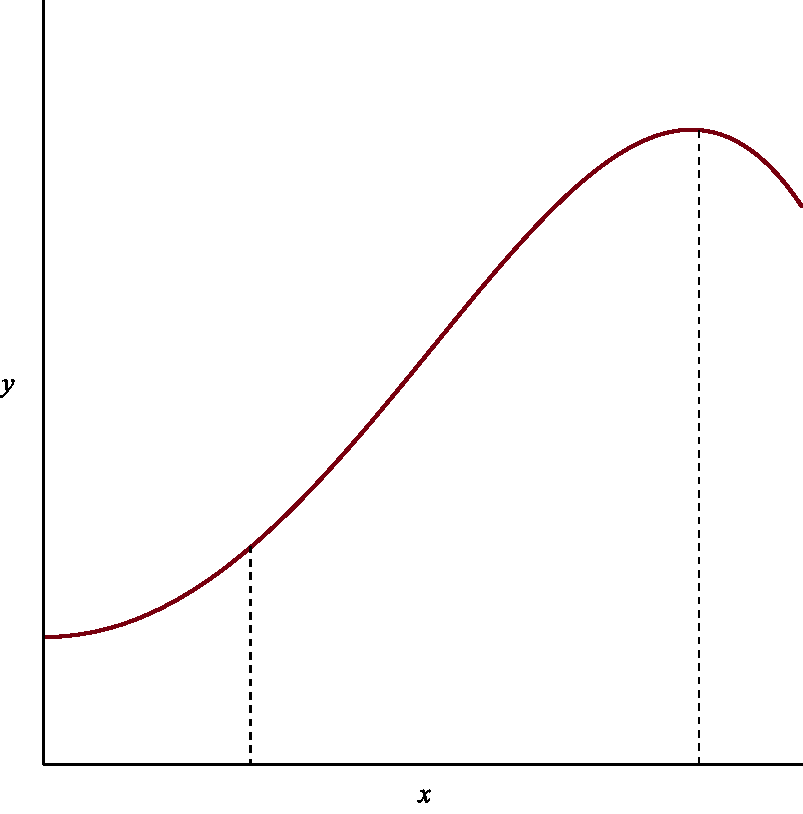
\includegraphics[width=0.6\textwidth]{arclength1.pdf}
%%   \end{figure}


%% Let $S$ be the arc length
%% and  $\Delta S$ a short section of it.

%%   \begin{figure}[H]
%%     \centering
%%    % \def\svgwidth{0.4\columnwidth}
%%     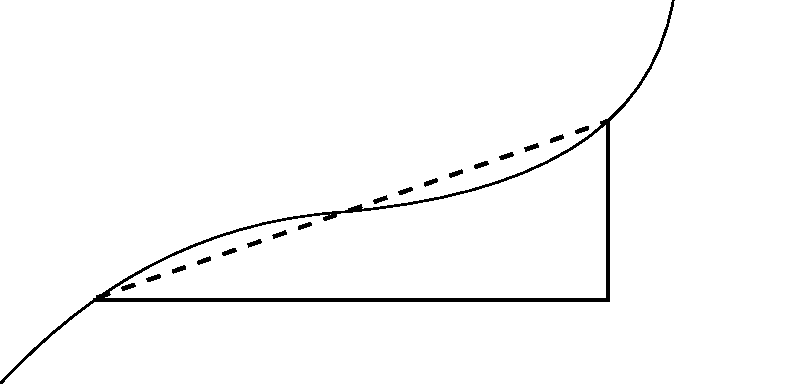
\includegraphics[width=0.6\textwidth]{arclengthdx.pdf}
%%   \end{figure}


%% By Pythagoras' Theorem,
%% \begin{eqnarray*}
%% \Delta S^2&\approx& \Delta x^2+\Delta y^2\\
%% \Rightarrow
%% \left(\dfrac{\Delta S}{\Delta x}\right)^2&\approx&1+\left(\dfrac{\Delta y}{\Delta x}\right)^2
%% \end{eqnarray*}
%% As $\Delta x\to0$ this becomes an identity
%% \begin{eqnarray*}
%% \left(\dfrac{d S}{d x}\right)^2&=&1+\left(\dfrac{d y}{d x}\right)^2\\
%% \Rightarrow
%% \dfrac{d S}{d x}&=&\sqrt{1+\left(\dfrac{d y}{d x}\right)^2}
%% \end{eqnarray*}
%% The arclength between $x=a$ and $x=b$ is then
%% \begin{eqnarray*}
%% S(a,b)&=&\int_a^b\dfrac{d S}{d x}dx\\
%% &=&\int_a^b\sqrt{1+\left(\dfrac{d y}{d x}\right)^2}dx.
%% \end{eqnarray*}

%% \begin{example}

%% Find the arc length of the graph of the function
%% \[
%% y=f(x)=\dfrac{x^3}6+\dfrac1{2x}
%% \]
%% on the interval $\left(\dfrac12,2\right)$.

%% Sketch the graph of $f(x)$ for $x>0$:

%% If $x=0$, $y$ is undefined.

%% We have $y=0$ if $\dfrac{x^3}6=-\dfrac1{2x}\Rightarrow x^4=-3$, hence never.

%% As $x\to0_+$, $y\to\infty$.
%% \\
%% As $x\to\infty$, $y\to\infty$ as well.

%% \begin{figure}[H]
%% \centering
%%  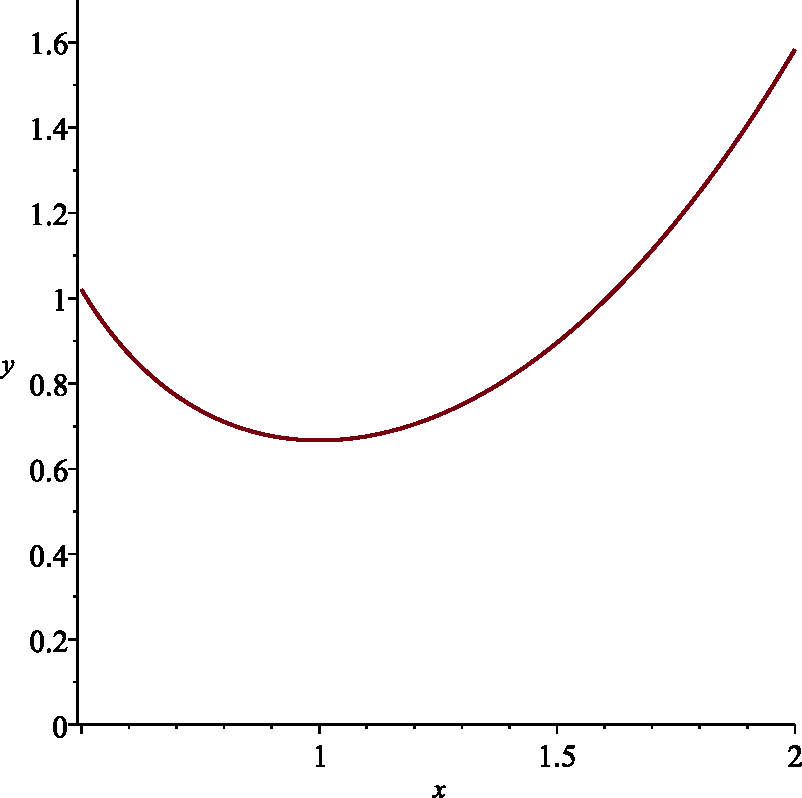
\includegraphics[width=0.5\textwidth]{arclengthexample.pdf}
%% %\captionsetup{labelformat=empty}
%% \end{figure}

%% Also, 
%% \[
%% \dfrac{d y}{d x}=\dfrac{3x^2}6-\dfrac1{2x^2}=\dfrac12\left(x^2-\dfrac1{x^2}\right).
%% \]
%% So
%% $\dfrac{d y}{d x}=0$ when $x^2-\dfrac1{x^2}=0
%% \Rightarrow
%% x^4=1
%% \Rightarrow
%% x=\pm1$.

%% Now, the arc length is
%% \[
%% S\left(\dfrac12,2\right)=\int_{\frac12}^2\sqrt{1+\left(\dfrac{d y}{d x}\right)^2}dx,
%% \]
%% with
%% \begin{eqnarray*}
%% 1+\left(\dfrac{d y}{d x}\right)^2
%% &=&1+\dfrac14\left(x^2-\dfrac1{x^2}\right)^2\\
%% &=&1+\dfrac14\left(x^4-2+\dfrac1{x^4}\right)\\
%% &=&\dfrac14\left(x^4+2+\dfrac1{x^4}\right)\\
%% &=&\dfrac14\left(x^2+\dfrac1{x^2}\right)^2.
%% \end{eqnarray*}
%% Thus,
%% \begin{eqnarray*}
%% S\left(\dfrac12,2\right)
%% &=&\int_{\frac12}^2\dfrac12\left(x^2+\dfrac1{x^2}\right)dx\\
%% &=&\dfrac12\left[\dfrac{x^3}3-\dfrac1{x}\right]_{\frac12}^2=\dfrac{33}{16}.
%% \end{eqnarray*}
%% \end{example}

%% \begin{example}

%% It can be shown that a hanging chain forms a curve (see Exercise Sheet 4 Q.5)
%% \[
%% y=\cosh(x).
%% \]
%% The arc length on the interval $\left(-a,a\right)$ is
%% \begin{eqnarray*}
%% S\left(-a,a\right)&=&\int_{-a}^a\sqrt{1+\left(\dfrac{d y}{d x}\right)^2}dx\\
%% &=&\int_{-a}^a\sqrt{1+\sinh^2(x)}dx\\
%% &=&\int_{-a}^a\cosh(x)dx
%% =%\\&=&
%% \Big[\sinh(x)\Big]_{-a}^a=2\sinh(a).
%% \end{eqnarray*}
%% \end{example}

%% \textbf{Warning. } Calculating arc length often leads to integrals we cannot evaluate, e.g. $y(x)=\sin(x)$ yields
%% \[
%% S=\int_a^b\sqrt{1+\cos^2(x)} \, dx=???
%% \]

%% \subsubsection*{Surface areas of revolutions} 

%% Given a curve $y(x)$ we can generate a surface (of revolution) by rotating the curve about the $x$-axis.

%% What is the area of such a surface?

%% \textbf{Idea. } 
%% Split the shell into thin strips

%%   \begin{figure}[H]
%%     \centering
%%    % \def\svgwidth{0.4\columnwidth}
%%     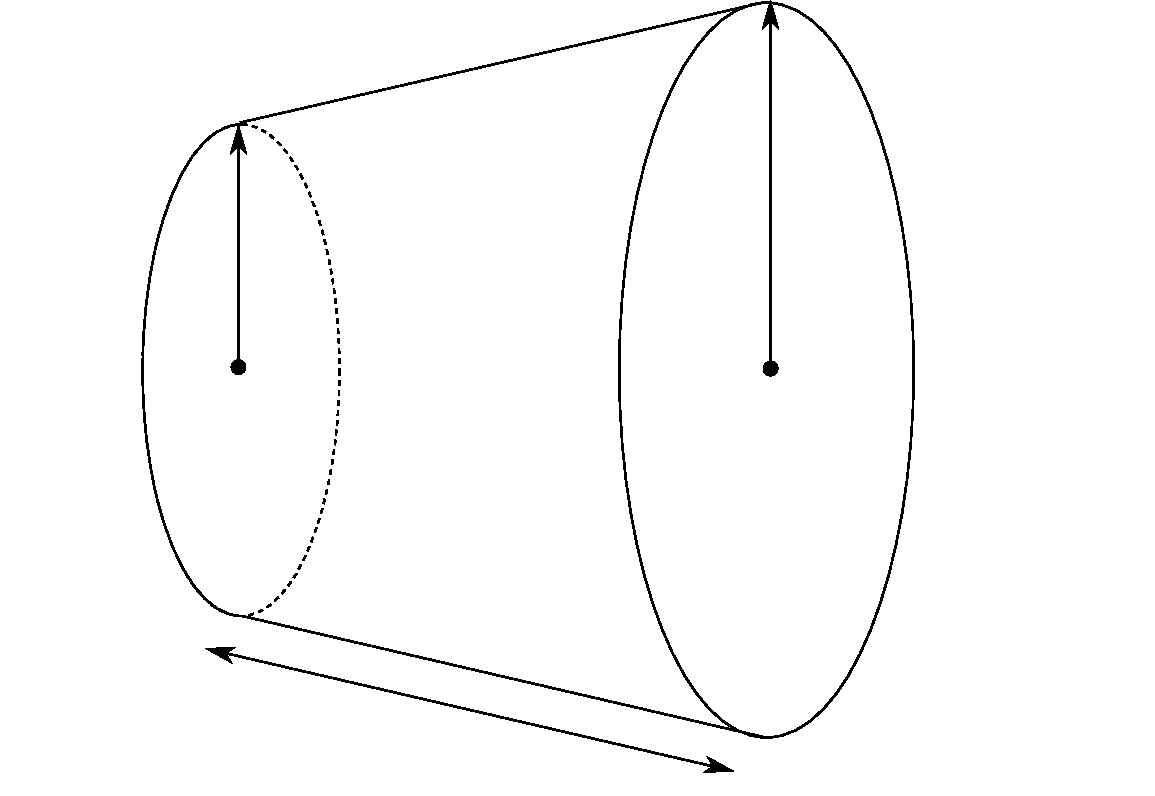
\includegraphics[width=0.6\textwidth]{frustum.pdf}
%%   \end{figure}

%% The area of the shell of a {\bf Conical Frustum} is $A=\pi (r_1+r_2)L$.

%% Thus, the area of the strip is approximately 
%% (set $r_1=y, r_2=y+\Delta y, L=\Delta S$)

%% \begin{eqnarray*}
%% \Delta A&\approx&\pi (y+(y+\Delta y))\cdot\Delta S\\
%% \Rightarrow\ \dfrac{\Delta A}{\Delta x}&=&2\pi \left(y+\frac12\Delta x\dfrac{\Delta y}{\Delta x}\right)\cdot\dfrac{\Delta S}{\Delta x}.
%% \end{eqnarray*}
%% As $\Delta x\to0$ 
%% $$
%% \dfrac{dA}{dx}=2\pi y\dfrac{dS}{dx}
%% \text{\qquad  as\quad} \dfrac{\Delta y}{\Delta x}\to\dfrac{dy}{dx} \text{ stays bounded.}
%% $$
%% Hence, using the previous arclength formula
%% \begin{eqnarray*}
%% A(a,b)&=&\int_a^b\dfrac{dA}{dx}dx
%% =%\\&=&
%% 2\pi \int_a^b y\sqrt{1+\left(\dfrac{d y}{d x}\right)^2}\ dx.
%% \end{eqnarray*}


%% \begin{example}

%% Consider the curve $y=\sqrt{1+x^2}$, creating a hyperboloid of revolution (the flipped cooling tower).

%%   \begin{figure}[H]
%%     \centering
%%     \def\svgwidth{0.5\columnwidth}
%%     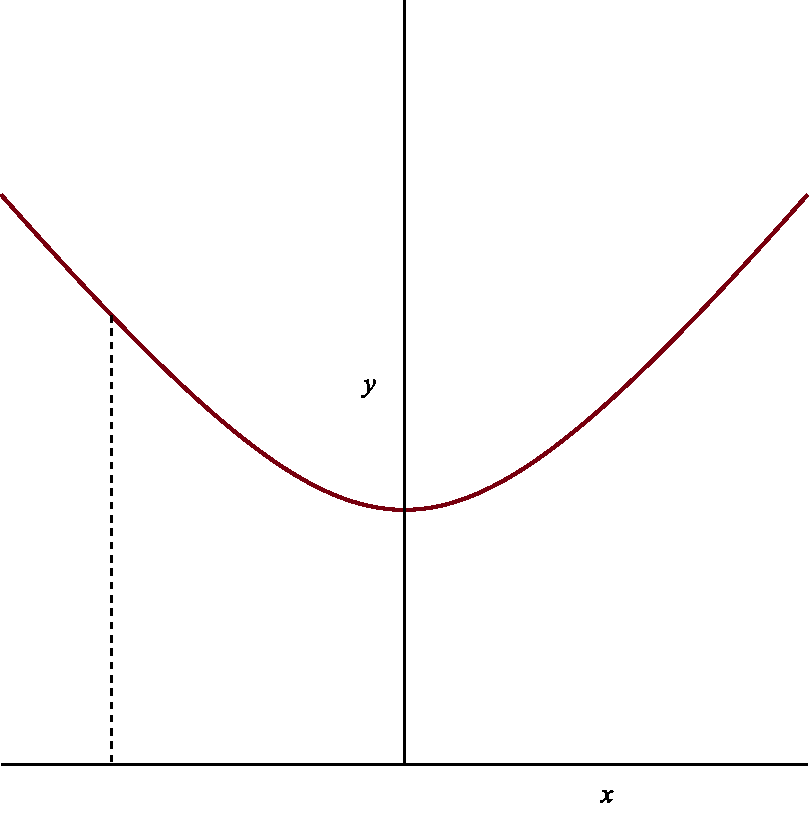
\includegraphics[width=0.6\textwidth]{hyperbola.pdf}
%%     %\captionsetup{labelformat=empty}
%%     \caption{$y=\sqrt{1+x^2}$}
%%   \end{figure}

%%   \begin{figure}[H]
%%     \centering
%%     \def\svgwidth{0.7\columnwidth}
%%     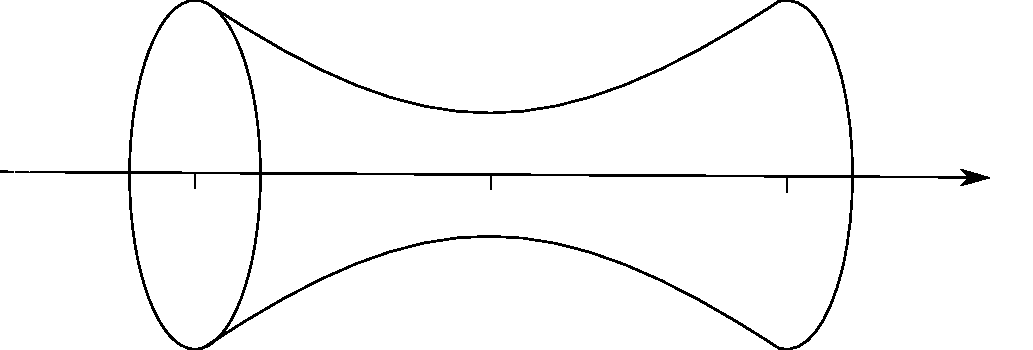
\includegraphics[width=0.6\textwidth]{hyperboloidrev.pdf}
%%     %\captionsetup{labelformat=empty}
%%     \caption{Hyperboloid of revolution}
%%   \end{figure}


%% As
%% \[
%% \dfrac{d y}{d x}=2x\dfrac12(1+x^2)^{-\frac12}=\dfrac x{\sqrt{1+x^2}}
%% \]
%% the surface area is
%% \begin{eqnarray*}
%% A(-a,a)
%% &=&2\pi \int_{-a}^a y\sqrt{1+\left(\dfrac{d y}{d x}\right)^2}\ dx\\
%% &=&2\pi \int_{-a}^a \sqrt{1+x^2}\sqrt{1+\dfrac {x^2}{1+x^2}}\ dx\\
%% &=&2\pi \int_{-a}^a \sqrt{1+x^2+x^2}\ dx\\
%% &=&2\pi \int_{-a}^a \sqrt{1+2x^2}\ dx.
%% \end{eqnarray*}
%% Hence, the substitution $u=\sqrt2 x$ yields $du=\sqrt 2 dx$ and so
%% \begin{eqnarray*}
%% A(-a,a)
%% &=&2\pi \int_{-\sqrt2 a}^{\sqrt2 a} \sqrt{1+u^2}\ \dfrac{du}{\sqrt2}\\
%% &=&\sqrt2\pi \cdot\dfrac12\left[u\sqrt{1+u^2}+\arcsinh(u)\right]_{-\sqrt2 a}^{\sqrt2 a}\\
%% &=&\sqrt2\pi \left[\sqrt2 a\sqrt{1+2a^2}+\arcsinh(\sqrt2 a)\right].
%% \end{eqnarray*}
%% \end{example}




%% \newpage
%% \section{Multivariable Differentiation}

So far we have worked only with functions in one variable (usually called $x$ or $t$).  In this chapter we will look at functions of multiple variables where those variables are allowed to be independent of one another.  The calculus of such functions is more complicated than the single variable case, and we will look at this in detail for functions of $2$ and $3$ variables.

\subsection{Functions of several variables}

  As always in this course, we will only deal with real functions of real variables.  Although we allow multiple variables, the value of the function will still be a single real number.

  \begin{definition}
    For a (non-zero) natural number $n$, a \emph{function $f$ of $n$ variables} is a function
      \[
        f \colon \mathbb{R}^n \longrightarrow \mathbb{R},
      \]
    or a function
      \[
        f \colon D \longrightarrow \mathbb{R},
      \]
    where $D \subset \mathbb{R}^n$.
  \end{definition}

  \subsubsection*{Remarks:}
    \begin{itemize}[topsep=0pt]
      \item We will focus on the cases when $n = 2$ and $n = 3$.
      \item As with the single variable case, we have to allow the domain to be a subset of $\mathbb{R}^n$, in case there are points at which the function is not defined (e.g. due to dividing by $0$, square roots of negatives, etc.).
      \item The codomain of our functions is always $\mathbb{R}$, \emph{not} $\mathbb{R}^n$.
    \end{itemize}

  \subsubsection*{Notation:}
    \begin{itemize}[topsep=0pt]
      \item For a function $f$ of $2$ variables, we write
        \[
          f(x, y)
        \]
      for the value of $f$ at the point $(x, y)$.
      \item Similarly, for a function $f$ of $3$ variables, we write
        \[
          f(x, y, z).
        \]
      \item For a function of $n$ variables, we write
        \[
          f(x_1, x_2, \dotsc, x_n).
        \]
    \end{itemize}

  \begin{examples}
  \
    \begin{enumerate}[topsep=0pt]
      \item Equation of a plane: linear expression in $x$ and $y$, e.g.
        \[
          f(x, y) = 3x - y + 2.
        \]
      \item Polynomials in $x$ and $y$, e.g.
        \[
          g(x, y) = x^3 + y^3 - 3x - 3y.
        \]
      \item We can include terms involving both $x$ and $y$:
        \[
          h(x, y) = x^2 + y^2 - \frac{1}{2}xy.
        \]
      \item A trigonometric example:
        \[
          k(x, y) = x\sin(y).
        \]
    \end{enumerate}
  \end{examples}

  We will use these examples throughout this chapter.  3D plots shown in the lecture.


\subsection{Partial derivatives}

  In this section we develop the tools for studying rates of change of functions of more than one variable.  As usual we do this using differentiation.

  We look at the two-variable case first (other cases are similar).  We are used to differentiating with respect to an independent variable, but now we have two independent variables, $x$ and $y$.

  Two possibilities:
    \begin{itemize}[topsep=0pt]
      \item Differentiate with respect to $x$; keep $y$ fixed.
      \item Differentiate with respect to $y$; keep $x$ fixed.
    \end{itemize}

  We can do either of these.  The derivatives we get are called \emph{partial derivatives}.

  \begin{definition}
    Given a function $f$ of two variables, if $(x_0, y_0)$ is a point in the domain of $f$, the \emph{partial derivative of $f$ with respect to $x$} is
    \[
      \frac{\partial f}{\partial x}(x_0, y_0) := \left. \frac{d}{dx}f(x, y_0) \right|_{x = x_0} = \lim_{\Delta x \rightarrow 0} \frac{f(x_0 + \Delta x, y_0) - f(x_0, y_0)}{\Delta x}.
    \]
    Similarly, the \emph{partial derivative of $f$ with respect to $y$} is
    \[
      \frac{\partial f}{\partial y}(x_0, y_0) := \left. \frac{d}{dx}f(x_0, y) \right|_{y = y_0} = \lim_{\Delta y \rightarrow 0} \frac{f(y_0, y_0 + \Delta y) - f(x_0, y_0)}{\Delta y}.
    \]
  \end{definition}

  This definition may look scary but the moral is fairly simple: if we fix $y$, $f$ becomes a function of $x$ only, and we can differentiate it with respect to $x$ in the usual way (and vice versa).

  \subsubsection*{Notation:}
  The partial derivatives are themselves functions of two variables $(x, y)$.  We write them either as
    \[
      \frac{\partial f}{\partial x}, \quad \frac{\partial f}{\partial y},
    \]
  or
    \[
      f_x(x, y), \quad f_y(x, y).
    \]
  The symbol $\partial$ is a stylised $d$ used mainly for partial derivatives.  It is derived from the Cyrillic alphabet.

  \subsubsection*{Interpretation}

  In the definition of $f_x(x, y)$, we treated $y$ as a constant (holding $y$ fixed) and differentiated with respect to $x$.  The act of fixing a value of $y$ corresponds to looking at a certain plane with an equation of the form $y = c$, a constant.  Such a plane intersects $z = f(x, y)$, as shown in figure (\ref{yfixed}).
%% \nextalt{Request description from lecturer or 3D object.}
%% \ifboolexpr{togl {clearprint} or togl {web}}
%% {
%%   \begin{figure}[H]
%%     \centering
%%     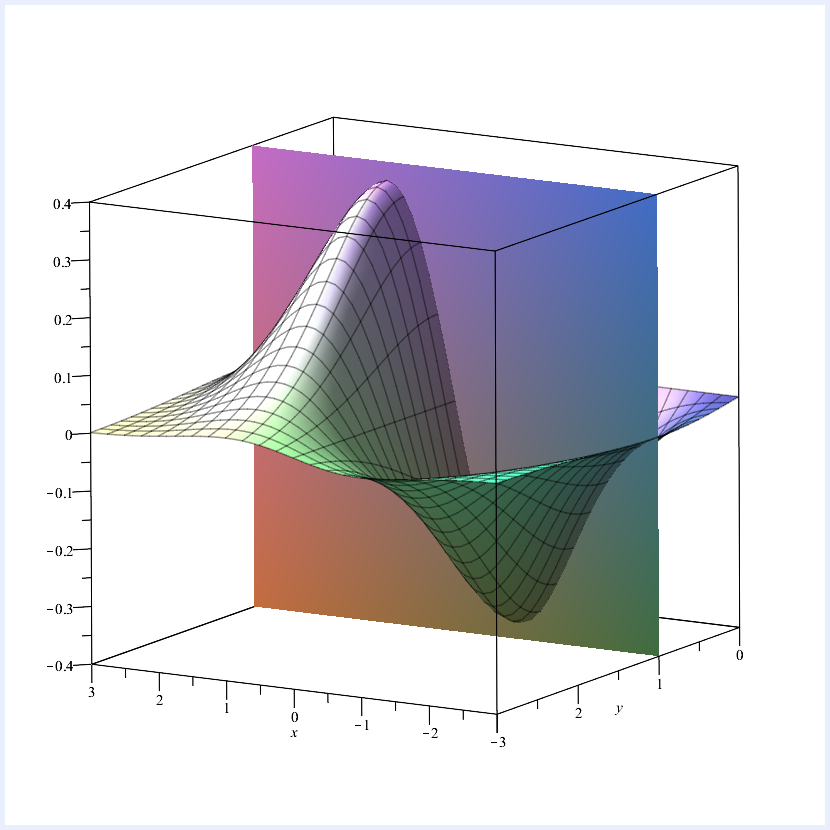
\includegraphics[width=0.75\textwidth]{yfixed.png}
%%     \caption{Plane intersecting $z = f(x, y)$}
%%     \label{yfixed}
%%   \end{figure}
%% }{
  \begin{figure}[H]
    \centering
    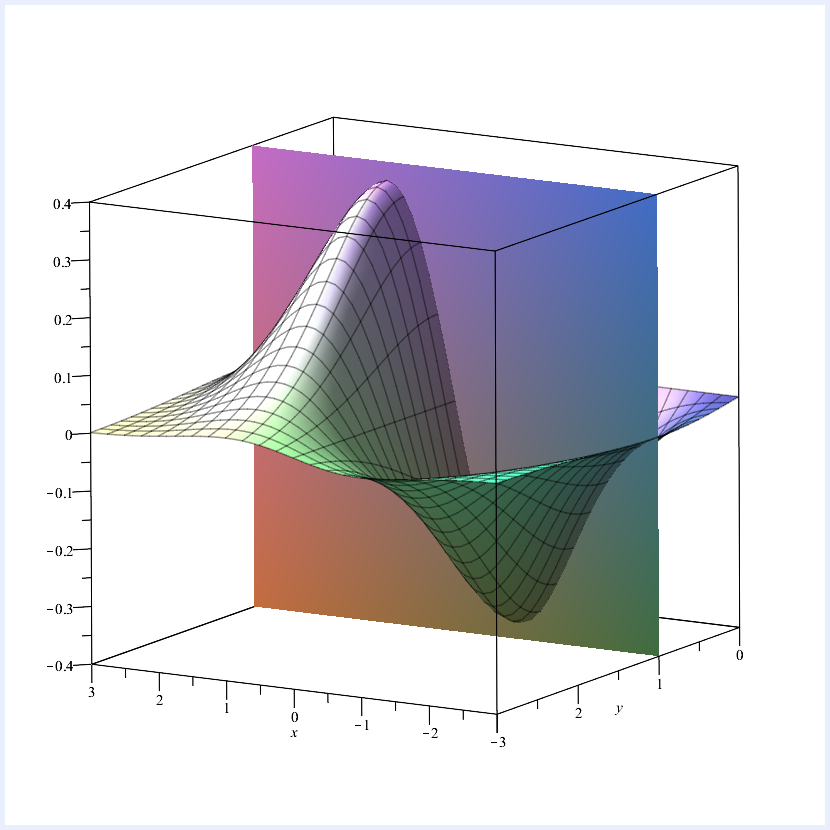
\includegraphics[width=0.51\textwidth]{yfixed.png}
    \caption{Plane intersecting $z = f(x, y)$}
    \label{yfixed}
  \end{figure}
%% }

  The intersection of the surface and the plane is a curve that depends on $x$.  The value of the partial derivative $f_x(x, y)$ at a particular point $(x, c)$ is the gradient of this curve for that particular $x$ value.  Similarly, for $f_y(x, y)$, the plane $x = c$ intersects $f(x, y)$ in a curve; $f_y(c, y)$ is the gradient of this curve for a given $y$ value.

  \begin{examples}
  \
    \begin{enumerate}
      \item $f(x, y) = 3x - y + 2$, then
        \[
          f_x(x, y) = 3, \quad f_y(x, y) = -1.
        \]
      \item $g(x, y) = x^3 + y^3 - 3x - 3y$, then
        \[
          g_x(x, y) = 3x^2 - 3, \quad g_y(x, y) = 3y^2 - 3.
        \]
      \item $h(x, y) = x^2 + y^2 - \frac{1}{2}xy$, then
        \[
          h_x(x, y) = 2x - \frac{1}{2}y, \quad h_y(x, y) = 2y - \frac{1}{2}x.
        \]
      \item $k(x, y) = x\sin(y)$, then
        \[
          k_x(x, y) = \sin(y), \quad k_y(x, y) = x\cos(y).
        \]
    \end{enumerate}
  \end{examples}

  \subsubsection*{Higher order partial derivatives}

  Partial derivatives are functions of two variables, so they have partial derivatives of their own.  The resulting functions are called \emph{second order partial derivatives}.  This is like the second derivative of a function of one variable, but now we have four possibilities:
    \[
      \frac{\partial^2 f}{\partial x^2} = \frac{\partial}{\partial x} \left( \frac{\partial f}{\partial x} \right) = f_{xx}, \quad\quad \frac{\partial^2 f}{\partial y^2} = \frac{\partial}{\partial y} \left( \frac{\partial f}{\partial y} \right) = f_{yy},
    \]
    \[
      \frac{\partial^2 f}{\partial y \partial x} = \frac{\partial}{\partial y} \left( \frac{\partial f}{\partial x} \right) = f_{xy}, \quad\quad \frac{\partial^2 f}{\partial x \partial y} = \frac{\partial}{\partial x} \left( \frac{\partial f}{\partial y} \right) = f_{yx}.
    \]
  The last two cases are called \emph{mixed second-order partial derivatives}.

  Similarly, third order, fourth order, etc. partial derivatives can be obtained by successive differentiation.

  % It's likely that there's not time to do all of these!  Possibly just do 2 and 3.
  \begin{examples}
  \
    \begin{enumerate}
      \item $f(x, y) = 3x - y + 2$, then
        \[
          f_{xx}(x, y) = 0, \quad f_{yy}(x, y) = 0,
        \]
        \[
          f_{xy}(x, y) = 0, \quad f_{yx}(x, y) = 0.
        \]
      \item $g(x, y) = x^3 + y^3 - 3x - 3y$, then
        \[
          g_{xx}(x, y) = 6x, \quad g_{yy}(x, y) = 6y,
        \]
        \[
          g_{xy}(x, y) = 0, \quad g_{yx}(x, y) = 0,
        \]
      \item $h(x, y) = x^2 + y^2 - \frac{1}{2}xy$, then
        \[
          h_{xx}(x, y) = 2, \quad h_{yy}(x, y) = 2,
        \]
        \[
          h_{xy}(x, y) = -\frac{1}{2}, \quad h_{yx}(x, y) = -\frac{1}{2}.
        \]
      \item $k(x, y) = x\sin(y)$, then
        \[
          k_{xx}(x, y) = 0, \quad k_{yy}(x, y) = -x\sin(y),
        \]
        \[
          k_{xy}(x, y) = \cos(y), \quad k_{yx}(x, y) = \cos(y).
        \]
    \end{enumerate}
  \end{examples}

  \subsubsection*{Equality of mixed partials}

  In the examples, the two mixed partials were equal.  This is true in general.

  \begin{theorem}[Clairaut's Theorem]  \label{thm:mixedpartials}
    Let $f$ be a function of two variables.  If $\dfrac{\partial^2 f}{\partial y \partial x}$ and $\dfrac{\partial^2 f}{\partial x \partial y}$ are continuous at a point $(a, b)$, then
    \[
      \dfrac{\partial^2 f}{\partial y \partial x}(a, b) = \dfrac{\partial^2 f}{\partial x \partial y}(a, b).
    \]
  \end{theorem}

  %\emph{Note:} An open disc is a circular region of the $(x, y)$-plane, not including the boundary of the circle.  Open discs are important in analysis.

  See Analysis 2B for a proof.	A version of Theorem~\ref{thm:mixedpartials} also holds in the $n$-variable case for $n > 2$.


\subsection{Critical points}
  % This section is currently probably too verbose.
  % I may also need to cut back on the environments -- there are a lot more than in the earlier sections and their use probably doesn't contribute much.

  In the one-variable case we can use the derivative of a function to find its critical points: maxima, minima, and points of inflection.  We can do something similar for functions of two variables, using partial derivatives.

  First, we want to know what kind of features we're trying to identify.  As in the one-variable case, we have \emph{maxima} and \emph{minima}, which can be either absolute (aka global) or relative (aka local) (see figure (\ref{absmaxmin})).

%% \nextalt{Request description from lecturer or 3D object.}
%% \ifboolexpr{togl {clearprint} or togl {web}}
%% {
%% \begin{figure}[!htbp]
%% \centering
%%  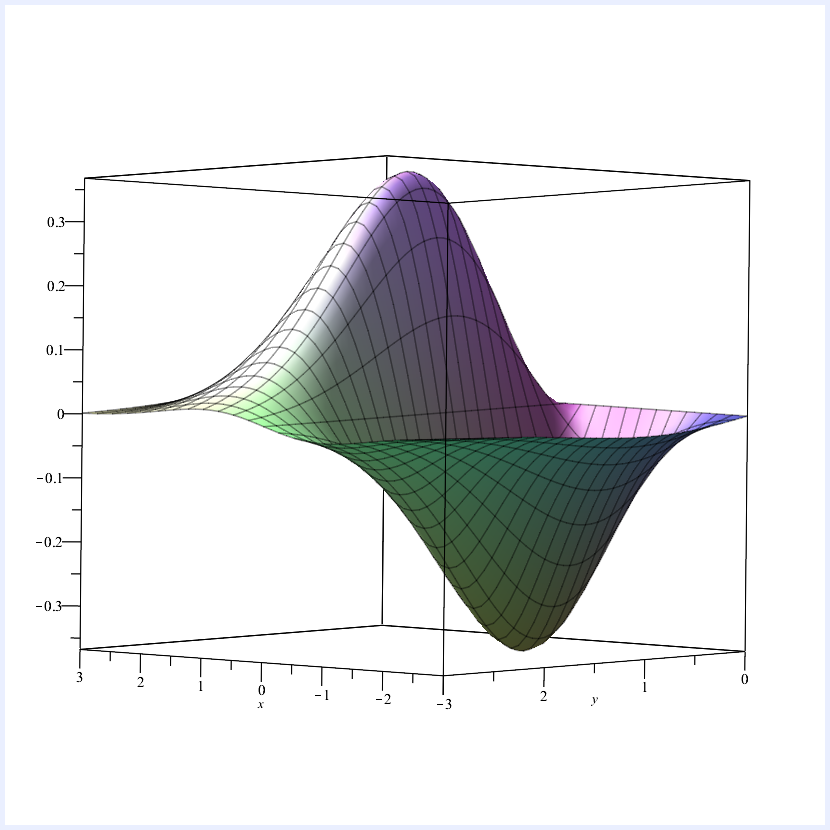
\includegraphics[width=0.75\textwidth]{maxandmin.png}
%% \caption{A function with an absolute maximum and absolute minimum.}
%% \label{absmaxmin}
%% \end{figure}
%% }{
\begin{figure}[!htbp]
\centering
 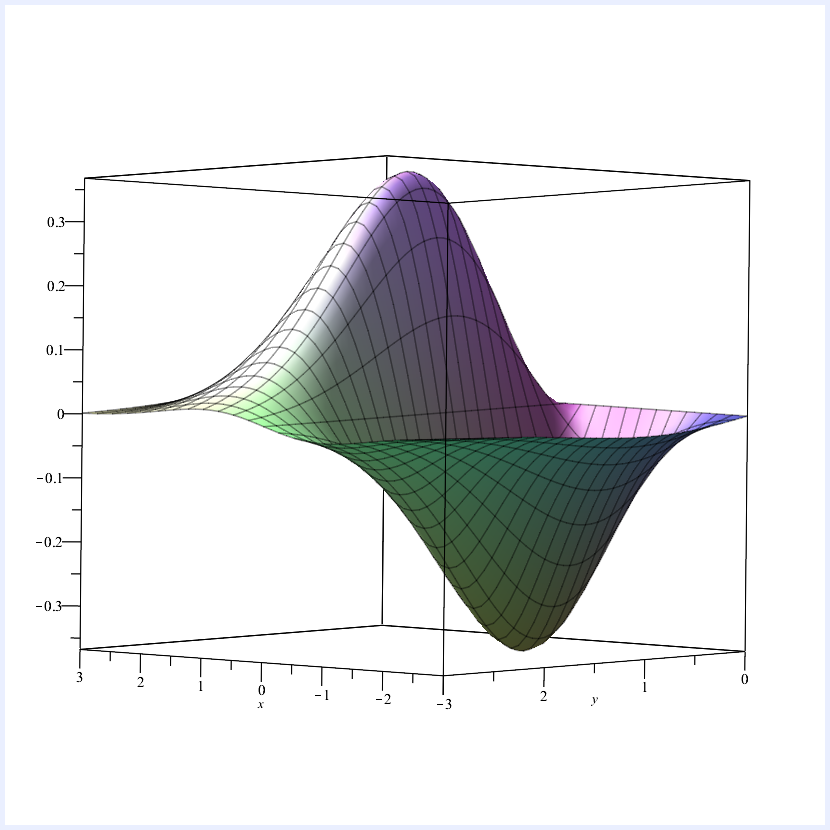
\includegraphics[width=0.55\textwidth]{maxandmin.png}
\caption{A function with an absolute maximum and absolute minimum.}
\label{absmaxmin}
\end{figure}
%% }

  The definitions of global maxima and minima are straightforward:

  \begin{definition}
    A function $f$ of two variables is said to have an \emph{absolute maximum} at $(x_0, y_0)$ if $f(x_0, y_0) \geq f(x, y)$ for all $(x, y)$.

    A function $f$ of two variables is said to have an \emph{absolute minimum} at $(x_0, y_0)$ if $f(x_0, y_0) \leq f(x, y)$ for all $(x, y)$.
  \end{definition}

\newpage

  The definitions of the relative versions are a bit fiddly (see figure (\ref{relmaxnabs})):

  \begin{definition}
    A function $f$ of two variables is said to have a \emph{relative maximum} at $(x_0, y_0)$ if there is a disc centred at $(x_0, y_0)$ such that $f(x_0, y_0) \geq f(x, y)$ for all $(x, y)$ inside the disc.

    A function $f$ of two variables is said to have a \emph{relative minimum} at $(x_0, y_0)$ if there is a disc centred at $(x_0, y_0)$ such that $f(x_0, y_0) \leq f(x, y)$ for all $(x, y)$ inside the disc.
  \end{definition}

%% \nextalt{Request description from lecturer or 3D object.}
%% \ifboolexpr{togl {clearprint} or togl {web}}
%% {
%% \begin{figure}[H]
%% \centering
%%  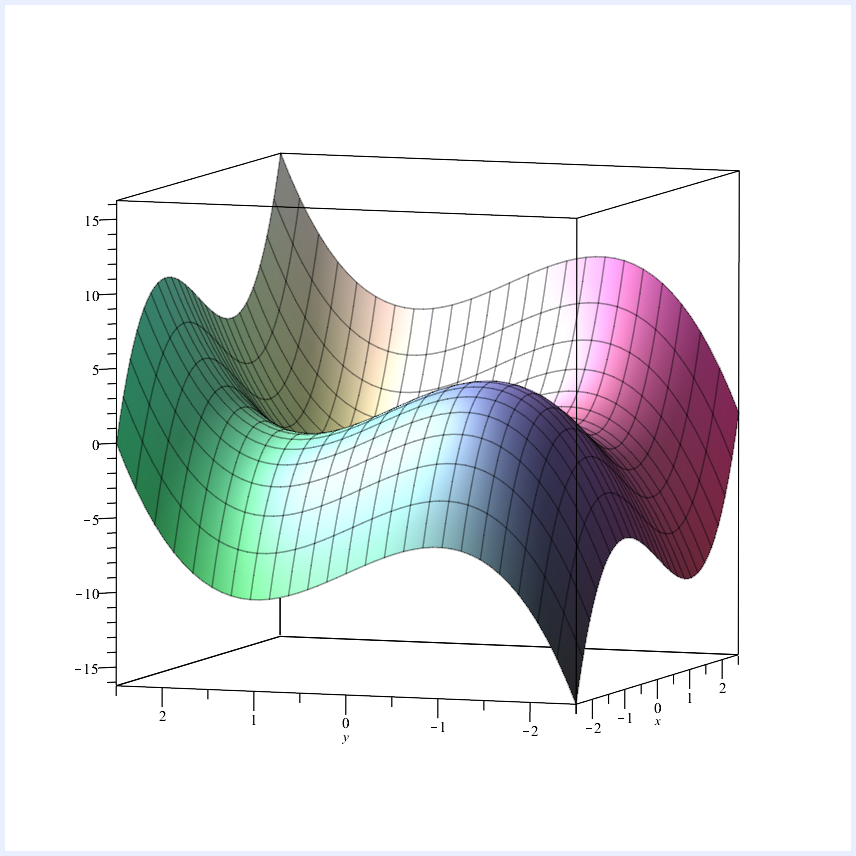
\includegraphics[width=0.75\textwidth]{relativemax.png}
%% \caption{A function with a relative maximum that is not absolute.}
%% \label{relmaxnabs}
%% \end{figure}
%% }{
\begin{figure}[H]
\centering
 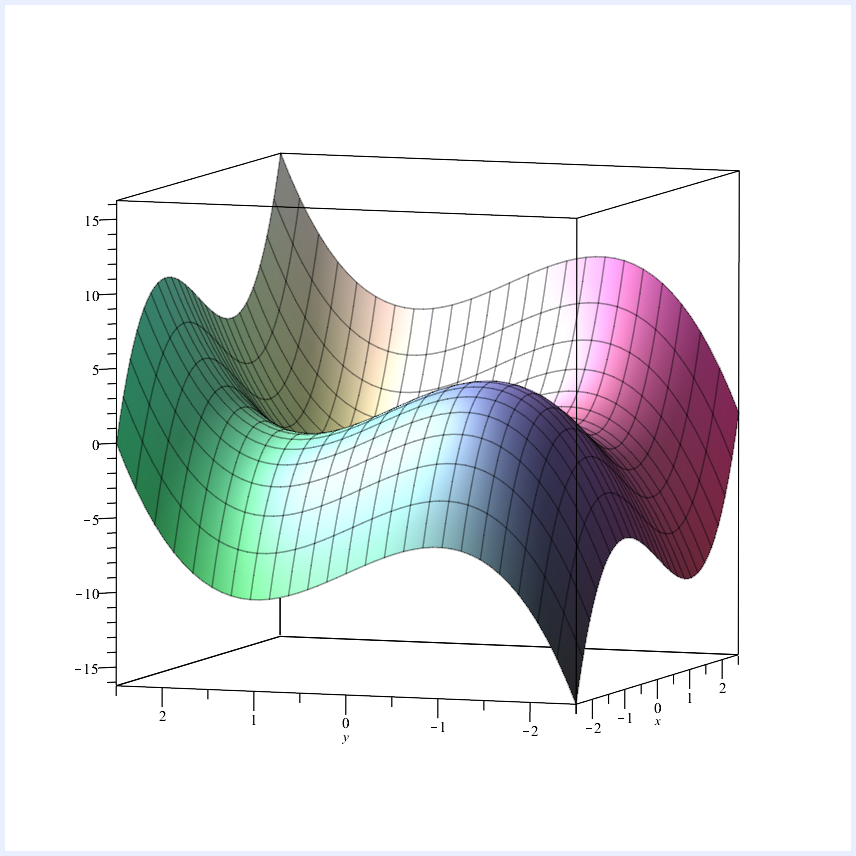
\includegraphics[width=0.55\textwidth]{relativemax.png}
\caption{A function with a relative maximum that is not absolute.}
\label{relmaxnabs}
\end{figure}
%%}

  % Technical definitions of maxima and minima.
  % Do I really need these?

  Collectively, maxima and minima are called \emph{extrema} (singular: extremum).  We can use partial derivatives to find most extrema (except for those on the boundaries of the domain), due to the following result:

  \begin{theorem}
    If $f$ has a relative extremum at $(x_0, y_0)$, and if the partial derivatives of $f$ exist at $(x_0, y_0)$, then
      \[
        \frac{\partial f}{\partial x}(x_0, y_0) = 0, \quad \frac{\partial f}{\partial y}(x_0, y_0) = 0.
      \]
  \end{theorem}

  The converse is not necessarily true: if the partial derivatives at a point are both $0$, that point is not guaranteed to be a relative extremum.

  \begin{definition}
    A point $(x_0, y_0)$ in the domain of a function $f(x, y)$ is called a \emph{critical point} if
      \[
        \frac{\partial f}{\partial x}(x_0, y_0) = 0, \quad \frac{\partial f}{\partial y}(x_0, y_0) = 0,
      \]
    or if one or both partial derivatives do not exist at $(x_0, y_0)$.
  \end{definition}

  As in the one-variable case, not all critical points are extrema.  A critical point that is not an extremum is called a \emph{saddle point} (figure (\ref{saddle})):

%% \nextalt{Request description from lecturer or 3D object.}
%% \ifboolexpr{togl {clearprint} or togl {web}}
%% {
%%   \begin{figure}[H]
%%     \centering
%%     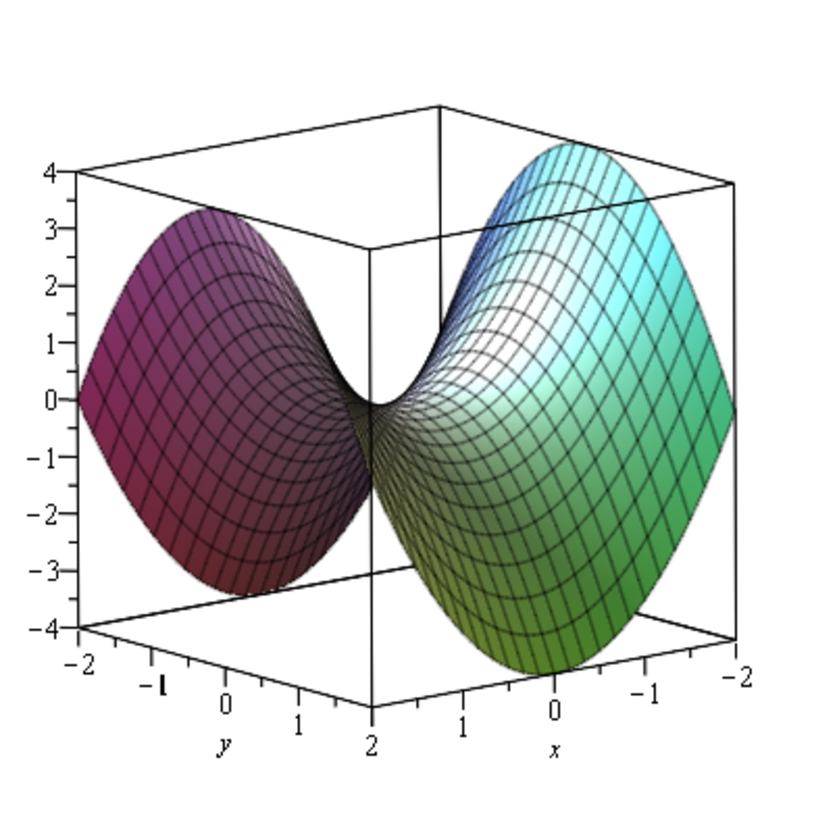
\includegraphics[width=0.75\textwidth]{paraboloid.pdf}
%%     \caption{Saddle point}
%%     \label{saddle}
%%   \end{figure}
%%   % Also, Pringles
%% }{
  \begin{figure}[H]
    \centering
    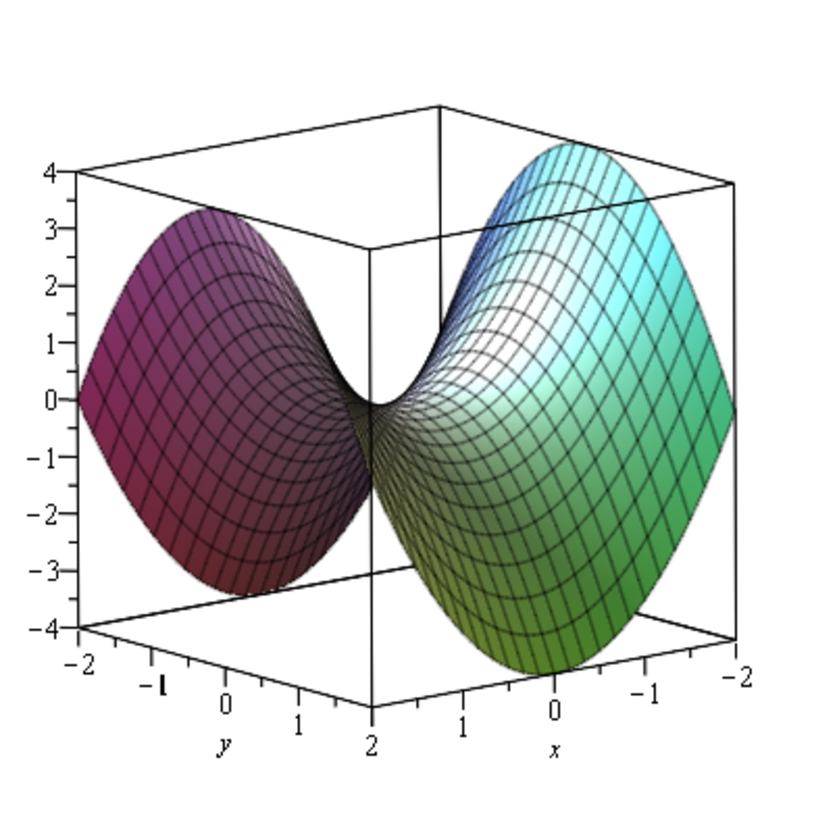
\includegraphics[width=0.6\textwidth]{paraboloid.pdf}
    \caption{Saddle point}
    \label{saddle}
  \end{figure}
  % Also, Pringles
%%}

  How do we tell if a critical point is an extremum?

  \begin{theorem}[Second Partials Test]
    Let $f$ be a function of two variables with continuous second-order partial derivatives in some disc centred at a critical point $(x_0, y_0)$, and let
    \[
      D = f_{xx}(x_0, y_0)f_{yy}(x_0, y_0) - f_{xy}(x_0, y_0)^2.
    \]
    \begin{enumerate}[label=(\alph*)]
      \item If $D > 0$ and $f_{xx}(x_0, y_0) > 0$, then $(x_0, y_0)$ is a relative minimum.
      \item If $D > 0$ and $f_{xx}(x_0, y_0) < 0$, then $(x_0, y_0)$ is a relative maximum.
      \item If $D < 0$, then $(x_0, y_0)$ is a saddle point.
      \item If $D = 0$, no conclusion can be drawn.
    \end{enumerate}
  \end{theorem}
	
	For a proof, see Analysis 2B; here we simply give some informal justification.
	
	Compare this with the one-variable version: suppose $f(x)$ has a critical point at $x_0$.  If $f''(x_0) < 0$, the gradient is decreasing as $x$ increases, so $x_0$ is a relative maximum.  Similarly, if $f''(x_0) > 0$, the gradient is increasing as $x$ increases, so $x_0$ is a relative minimum.
	
	Now consider the two-variable case.  If $D > 0$, then $f_{xx}$ and $f_{yy}$ have the same sign at $(x_0, y_0)$, and $f_{xy}$ is comparatively small, indicating little interaction between the two variables.  Thus, similar to the one-variable case, either $f_{xx}$, $f_{yy} < 0$ and the critical point is a relative maximum, or $f_{xx}$, $f_{yy} > 0$ and it is a relative minimum.
	
	If $D < 0$, then either $f_{xx}$ and $f_{yy}$ have different signs at $(x_0, y_0)$, or $f_{xy}$ is comparatively large and there is a lot of interaction between variables (or both).  Either of these possibilities leads to a saddle point.

  \begin{note}
    The $D$ stands for \emph{determinant}, so-called since it determines the nature of critical point.  It can also be expressed as the determinant of a matrix whose entries are the second order partials.
  \end{note}
  % Might be worth deformalising this, getting rid of most environments and making it notier/chattier.

  \begin{example}
    Recall the function $g(x, y) = x^3 + y^3 - 3x - 3y$.  The critical points occur when
      \[
        g_x(x, y) = 3x^2 - 3 = 0, \quad g_y(x, y) = 3y^3 - 3 = 0,
      \]
    i.e. when
      \[
        x^2 = 1, y^2 = 1.
      \]
    So the critical points are
      \[
        (1, 1), (-1, 1), (1, -1), (-1, -1).
      \]
    We use the second partial test:
      \[
        D = g_{xx}(x, y)g_{yy}(x, y) - g_{xy}(x, y)^2 = 6x \times 6y - 0 \times 0 = 36xy,
      \]
    so
      \begin{itemize}
        \item at $(1, 1)$, $D > 0$ and $g_{xx}(1, 1) > 0$, so $(1, 1)$ is a relative minimum;
        \item at $(-1, 1)$, $D < 0$, so $(-1, 1)$ is a saddle point;
        \item at $(1, -1)$, $D < 0$, so $(1, -1)$ is a saddle point;
        \item at $(-1, -1)$, $D > 0$, $g_{xx}(-1, -1) < 0$, so $(-1, -1)$ is a relative maximum.
      \end{itemize}
  \end{example}


  \subsection{Chain rules}

  As in the one-variable case, there are chain rules for differentiating composite functions of several variables.  There are various cases.

  \subsubsection*{Variables depend on $t$}

  The simplest case is the following:  let $f$ be a differentiable function of two variables $x$ and $y$, where $x = x(t)$, $y = y(t)$ are differentiable functions of $t$.  Then $f(x(t), y(t))$ is a differentiable function of $t$, and
    \[
      \frac{df}{dt} = \frac{\partial f}{\partial x}\frac{dx}{dt} + \frac{\partial f}{\partial y}\frac{dy}{dt}.
    \]

  The three-variable version is similar: let $f$ be a differentiable function of three variables $x$, $y$ and $z$, where $x = x(t)$, $y = y(t)$, $z = z(t)$ are differentiable functions of $t$.  Then $f(x(t), y(t), z(t))$ is a differentiable function of $t$, and
    \[
      \frac{df}{dt} = \frac{\partial f}{\partial x}\frac{dx}{dt} + \frac{\partial f}{\partial y}\frac{dy}{dt} + \frac{\partial f}{\partial z}\frac{dz}{dt}.
    \]

  \begin{examples} \
    \begin{enumerate}
      \item We begin with a simple example where we can easily find the answer directly.  Let
        \[
          z = x^2 y, \quad x = t^3, \quad y = t^2.
        \]
      Then, by the chain rule,
        \begin{align*}
          \frac{dz}{dt} & = \frac{\partial z}{\partial x}\frac{dx}{dt} + \frac{\partial z}{\partial y}\frac{dy}{dt}  \\
          & = 2xy \times 3t^2 + x^2 \times 2t  \\
          & = (2t^5)(3t^2) + (t^6)(2t)  \\
          & = 6t^7 + 2t^7 = 8t^7.
        \end{align*}
      We can check this directly by writing $z$ purely in terms of $t$:
        \[
          z = x^2 y = t^6 \times t^2 = t^8,
        \]
      so
        \[
          \frac{dz}{dt} = 8t^7.
        \]
      \item Let
        \[
          z = \sqrt{y^2 - xy}, \quad x = \cos(\theta), \quad y = \sin(\theta).
        \]
      Find the value of $\displaystyle \frac{dz}{d\theta}$ at $\displaystyle \theta = \frac{\pi}{2}$.

      By the chain rule,
        \begin{align*}
          \frac{dz}{d\theta} & = \frac{\partial z}{\partial x}\frac{dx}{d\theta} + \frac{\partial z}{\partial y}\frac{dy}{d\theta}  \\
          & = \frac{-y}{2\sqrt{y^2 - xy}} \times (-\sin(\theta)) + \frac{2y - x}{2\sqrt{y^2 - xy}} \times \cos(\theta).
        \end{align*}
      Now, at $\displaystyle \theta = \frac{\pi}{2}$,
        \[
          x = \cos\left(\frac{\pi}{2}\right) = 0, \quad y = \sin\left(\frac{\pi}{2}\right) = 1,
        \]
      so
        \[
          \frac{dz}{d\theta}\left(\frac{\pi}{2}\right) = \frac{-1}{2\sqrt{1 - 0}}\times(-1) + \frac{2 - 0}{2\sqrt{1 - 0}}\times 0 = \frac{1}{2}.
        \]
    \end{enumerate}
  \end{examples}

  \subsubsection*{Some useful applications of the chain rule}

  \begin{enumerate}
    \item Deriving rules of differentiation, e.g. the Product Rule.  What is
      \[
        \frac{d}{dx}(u(x)v(x)) \text{?}
      \]
      We can think of this as
      \[
        f(u, v) = uv
      \]
      where $u = u(x)$, $v = v(x)$ are functions of $x$.  By the chain rule
      \[
        \frac{df}{dx} = \frac{\partial f}{\partial u}\frac{du}{dx} + \frac{\partial f}{\partial v}\frac{dv}{dx}.
      \]
      We have
      \[
        \frac{\partial f}{\partial u} = v, \quad \frac{du}{dx} = u'(x), \quad \frac{\partial f}{\partial v} = u, \quad \frac{dv}{dx} = v'(x),
      \]
      so
      \[
        \frac{df}{dx} = v(x)u'(x) + u(x)v'(x).
      \]
      Similarly, we can derive the quotient rule.

      We can also derive a rule for differentiating functions of the form
        \[
          f(x) = u(x)^{v(x)}.
        \]
      (See Worksheet 7, exercise 5.)
      % This is likely to change!
    \item Differentiating $f(x, y)$, where $y$ depends on $x$.

    Think of this as $f(u, y)$, where
      \[
        u = u(x) = x, \quad y = y(x).
      \]
    Then $\displaystyle \frac{du}{dx} = 1$, so by the chain rule
      \[
        \frac{df}{dx} = \frac{\partial f}{\partial u}\frac{du}{dx} + \frac{\partial f}{\partial y}\frac{dy}{dx} = \frac{\partial f}{\partial x} + \frac{\partial f}{\partial y}\frac{dy}{dx}.
      \]
  \end{enumerate}


  \subsubsection*{Variables depend on $u$ and $v$}

  In the next case, the variables are themselves functions of two variables, $u$ and $v$.

  Let $f$ be a differentiable function of two variables $x$ and $y$, where
    \[
      x = x(u, v), \quad y = y(u, v)
    \]
  are differentiable functions of $u$ and $v$.  Then $f(x(u, v), y(u, v))$ is a differentiable function of $u$ and $v$, and its partial derivatives are given by
    \begin{align*}
      \frac{\partial f}{\partial u} & = \frac{\partial f}{\partial x}\frac{\partial x}{\partial u} + \frac{\partial f}{\partial y}\frac{\partial y}{\partial u},  \\
      \frac{\partial f}{\partial v} & = \frac{\partial f}{\partial x}\frac{\partial x}{\partial v} + \frac{\partial f}{\partial y}\frac{\partial y}{\partial v}.
    \end{align*}

  \begin{example}
    Let
      \[
        z = e^{xy}, \text{ where } x = u^2 + v, \quad y = u - v^2.
      \]
    Then, by the chain rule,
      \begin{align*}
        \frac{\partial z}{\partial u} & = \frac{\partial z}{\partial x}\frac{\partial x}{\partial u} + \frac{\partial z}{\partial y}\frac{\partial y}{\partial u}  \\
        & = ye^{xy} \times 2u + xe^{xy}  \\
        & = (2uy + x)e^{xy}  \\
        & = (3u^2 - 2uv^2 + v)e^{(u^2 + v)(u - v^2)},
      \end{align*}
    and
      \begin{align*}
        \frac{\partial z}{\partial v} & = \frac{\partial z}{\partial x}\frac{\partial x}{\partial v} + \frac{\partial z}{\partial y}\frac{\partial y}{\partial v}  \\
        & = ye^{xy} - 2vxe^{xy}  \\
        & = (y - 2vx)e^{xy}  \\
        & = (u - 2u^2v - 3v^2)e^{(u^2 + v)(u - v^2)}.
      \end{align*}
  \end{example}

  As in the previous case, there is a version of this chain rule for functions of $3$ variables; and, in fact, both cases also have versions for functions of $n$ variables.  We won't cover these in this course, but they look very similar to the chain rules we have seen.





% NEW SECTION STARTS HERE.




\newpage

\section{Multivariable Integration}

\subsection{Double integrals}

  We have seen integration of functions of one variable (which we now refer to as ``single integration'').  We now move on to definite integration of functions of two variables.

  \begin{tabular}{p{0.5\textwidth}|p{0.5\textwidth}}
    \emph{Single integrals:} & \emph{Double integrals:}  \\
    Area under a curve. & Volume under a surface.  \\
    Integrate over an interval of $x$-values. & Integrate over a region of the $(x, y)$-plane.  \\
    Evaluate using indefinite integral. & Evaluate using partial integration.  \\
  \end{tabular}

  \subsubsection*{Regions}

  Double integrals are performed over a region of the plane -- there are a lot more possibilities for the shape of this region than there were in one-dimension, where we always used an interval.

  The double integral of a function $f(x, y)$ over a region $R$ is denoted
    \[
      \iint_R f(x, y) \, dA,
    \]
  where $dA$ should be read as ``with respect to area $A$''.

  This gives the volume of the solid between the region $R$ of the $(x, y)$-plane and the surface $z = f(x, y)$, pictured in figure (\ref{doubleintegral3d}).
%% \nextalt{Request description from lecturer or 3D object.}
%% \iftoggle{web}
%% {
%%   \begin{figure}[H]
%%     \centering
%%     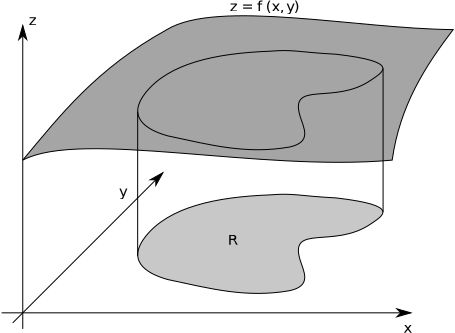
\includegraphics[width=0.6\textwidth]{doubleintegral3d.svg}
%%     \caption{Volume between region $R$ and surface $z$}
%%     \label{doubleintegral3d}
%%   \end{figure}
%% }{
%% \iftoggle{clearprint}{
%%   \begin{figure}[!htpb]
%%     \centering
%%     \def\svgwidth{0.7\columnwidth}
%%     \input{figures/latex/doubleintegral3d.pdf_tex}
%%     \caption{Volume between region $R$ and surface $z$}
%%     \label{doubleintegral3d}
%%   \end{figure}
%% }{
  \begin{figure}[H]
    \centering
    \def\svgwidth{0.6\columnwidth}
    \input{figures/latex/doubleintegral3d.pdf_tex}
    \caption{Volume between region $R$ and surface $z$}
    \label{doubleintegral3d}
  \end{figure}
%% }
%% }


  % Could put the technical, limit based definition here, or a note about how there is one.
  % It is somewhat hellish and definitely non-examinable.

  \subsubsection*{Properties of double integrals}

  Like single integrals, double integrals satisfy the usual linearity conditions:
    \begin{itemize}
      \item For a constant $c$,
    \[
      \iint_R cf(x, y) \, dA = c\iint_R f(x, y) \, dA;
    \]
      \item For functions $f(x, y)$ and $g(x, y)$,
    \[
      \iint_R f(x, y) + g(x, y) \, dA = \iint_R f(x, y)\, dA + \iint_R g(x, y) \, dA.
    \]
    \end{itemize}

  Also, if the region $R$ can be subdivided into regions $R_1$ and $R_2$ (figure (\ref{regionsubdivision})), then
    \[
      \iint_R f(x, y) \, dA = \iint_{R_1} f(x, y) \, dA + \iint_{R_2} f(x, y) \, dA.
    \]

%% \nextalt{Request description from lecturer or tactile diagram.}
%% \iftoggle{web}
%% {
%%   \begin{figure}[H]
%%     \centering
%%     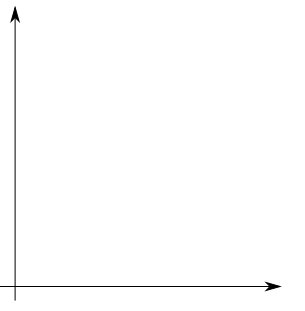
\includegraphics[width=0.4\textwidth]{regionsubdivision.svg}
%%     \caption{Region subdivision}
%%     \label{regionsubdivision}
%%   \end{figure}
%% }{
%% \iftoggle{clearprint}{
%%   \begin{figure}[!hbtp]
%%     \centering
%%     \def\svgwidth{0.4\columnwidth}
%%     \input{figures/latex/regionsubdivision.pdf_tex}
%%     \caption{Region subdivision}
%%     \label{regionsubdivision}
%%   \end{figure}
%% }{
  \begin{figure}[H]
    \centering
    \def\svgwidth{0.4\columnwidth}
    \input{figures/latex/regionsubdivision.pdf_tex}
    \caption{Region subdivision}
    \label{regionsubdivision}
  \end{figure}
%% }
%% }

  \subsubsection*{Evaluating double integrals with iterated integration}
	% Also changed "partial" to "iterated" in the title.  Which is more common?
	% The term "partial integration" does appear later as well.
	
	% I have rewritten the beginning of this section, with more justification.

  We will express the process of evaluating double integrals in terms of two single integrals: one with respect to $x$, one with respect to $y$.  We will start with the simplest possible regions (rectangles), then look at some more complicated ones.

  Suppose we want to evaluate the double integral of a function $f(x, y)$ over a rectangular region $R = [a, b] \times [c, d]$ (figure (\ref{rectangularregion2})).  
	
%% \nextalt{Request description from lecturer or tactile diagram.}
%% \iftoggle{web}
%% {
%%   \begin{figure}[H]
%%     \centering
%%     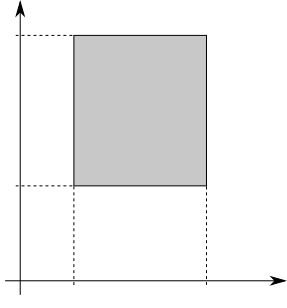
\includegraphics[width=0.45\textwidth]{rectangularregion2.svg}
%%     \caption{Rectangular region $R = [a, b] \times [c, d]$}
%%     \label{rectangularregion2}
%%   \end{figure}
%% }{
%% \iftoggle{clearprint}{
%%   \begin{figure}[!hbt]
%%     \centering
%%     \def\svgwidth{0.45\columnwidth}
%%     \input{figures/latex/rectangularregion2.pdf_tex}
%%     \caption{Rectangular region $R = [a, b] \times [c, d]$}
%%     \label{rectangularregion2}
%%   \end{figure}
%% }{
  \begin{figure}[H]
    \centering
    \def\svgwidth{0.45\columnwidth}
    \input{figures/latex/rectangularregion2.pdf_tex}
    \caption{Rectangular region $R = [a, b] \times [c, d]$}
    \label{rectangularregion2}
  \end{figure}
%% }
%% }
	
	Geometrically, this double integral is the volume $V$ of a solid. 	For a fixed value of $y$, the cross-sectional area of this solid is given by
    \[
      \int_a^b f(x, y) \, dx,
    \]
	by which we mean: integrate with respect to $x$, treat $y$ as a constant.  The result is a function of $y$.  Now suppose $y$ varies by a small increment $\Delta y$, giving a thin slice of the volume.  We can approximate the volume of the slice as
	  \[
		  \Delta V \approx \Delta y \int_a^b f(x, y) \, dx,
		\]
	the volume of a prism.  Thus
	  \[
		  \frac{\Delta V}{\Delta y} \approx \int_a^b f(x, y) \, dx.
		\]
	As $\Delta y \to 0$, this becomes an identity:
	  \[
		  \frac{dV}{dy} = \int_a^b f(x, y) \, dx.
		\]
	The volume from $y = c$ to $y = d$ is then
	  \[
		  \iint_R f(x, y) \, dA = \int_c^d \int_a^b f(x, y) \, dx \, dy.
		\]
		
	Notice that we could equally well have integrated with respect to $y$ first, to find the cross-sectional area for a fixed value of $x$, then integrated with respect to $x$ -- either order of integration would have given the volume of the solid, and therefore the same result.
	
	  \begin{theorem}[Fubini's Theorem -- special case]
    Let $R$ be the rectangle defined by
      \[
        a \leq x \leq b, \quad c \leq y \leq d.
      \]
    If $f(x, y)$ is continuous on $R$ then
    \[
      \iint_R f(x, y) \, dA = \int_c^d \int_a^b f(x, y) \, dx \, dy = \int_a^b \int_c^d f(x, y) \, dy \, dx.
    \]
  \end{theorem}

  \begin{example}
    Evaluate the double integral
      \[
        \iint_R 2xy \, dA
      \]
    where $R$ is the region defined by $1 \leq x \leq 3$, $2 \leq y \leq 4$.

    Using partial integration there are two possibilities: integrate first with respect to $x$, then $y$; or integrate first with respect to $y$, then $x$.  We will do both, then compare.
    \begin{align*}
      \int_2^4 \int_1^3 2xy \, dx \, dy & = \int_2^4 \left[ \int_1^3 2xy \, dx \right] dy  \\
      & = \int_2^4 \left[ x^2 y \right]_1^3 \, dy  \\
      & = \int_2^4 9y - y \, dy = \int_2^4 8y \, dy  \\
      & = \left[ 4y^2 \right]_2^4 = 4 \times 16 - 4 \times 4 = 48.
    \end{align*}
    \begin{align*}
      \int_1^3 \int_2^4 2xy \, dy \, dx & = \int_1^3 \left[ \int_2^4 2xy \, dy \right] dx  \\
      & = \int_1^3 \left[ xy^2 \right]_2^4 \, dx  \\
      & = \int_1^3 16x - 4x \, dx = \int_1^3 12x \, dx  \\
      & = \left[ 6x^2 \right]_1^3 = 6 \times 9 - 6 \times 1 = 48.
    \end{align*}
  So
  \[
    \int_2^4 \int_1^3 2xy \, dx \, dy = \int_1^3 \int_2^4 2xy \, dy \, dx.
  \]
  \end{example}
	

  \subsubsection*{Double integrals over non-rectangular domains}
	
	% There doesn't seem to be a sensible place to mention that this is using a more general version of Fubini's Theorem.

  In general this is very difficult, owing to the wide variety of possibilities for regions of the plane.  We'll look at certain types of non-rectangular regions that we can deal with.

  Consider a double integral
    \[
      \int_a^b \int_c^d f(x, y) \, dy \, dx.
    \]
  The inner partial integral (with respect to $y$) must give a function of $x$.  If $c$ and $d$ are functions of $x$, the resulting partial integral is still a function of $x$.  This allows us to integrate over regions of the form (figure (\ref{typeiregion})).
%% \nextalt{Request description from lecturer or tactile diagram.}
%% \iftoggle{web}
%% {
%%   \begin{figure}[H]
%%     \centering
%%     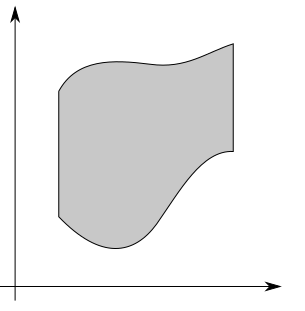
\includegraphics[width=0.4\textwidth]{typeiregion.svg}
%%     \caption{Type I region}
%%     \label{typeiregion}
%%   \end{figure}
%% }{
  \begin{figure}[H]
    \centering
    \def\svgwidth{0.4\columnwidth}
    \input{figures/latex/typeiregion.pdf_tex}
    \caption{Type I region}
    \label{typeiregion}
  \end{figure}
%% }

  The integral looks like
    \[
      \int_a^b \int_{g_1(x)}^{g_2(x)} f(x, y) \, dy \, dx.
    \]

  The outer limits must still be constant to give a numerical answer.

  Similarly, we can integrate over a region of the form (figure (\ref{typeiiregion}))
%% \nextalt{Request description from lecturer or tactile diagram.}
%% \iftoggle{web}
%% {
%%   \begin{figure}[H]
%%     \centering
%%     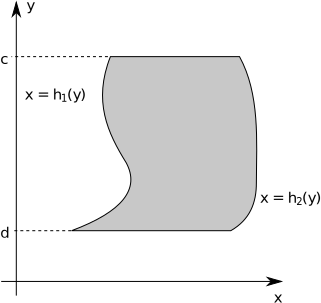
\includegraphics[width=0.47\textwidth]{typeiiregion.svg}
%%     \caption{Type II region}
%%     \label{typeiiregion}
%%   \end{figure}
%% }{
  \begin{figure}[H]
    \centering
    \def\svgwidth{0.47\columnwidth}
    \input{figures/latex/typeiiregion.pdf_tex}
    \caption{Type II region}
    \label{typeiiregion}
  \end{figure}
%% }
  using
    \[
      \int_c^d \int_{h_1(y)}^{h_2(y)} f(x, y) \, dx \, dy.
    \]

  % NOTE: I have cut two of these examples, one of which had a mistake, so save time since they took a whole lecture last year.
  \begin{examples}  
  \quad
    \begin{enumerate}
    \item Evaluate the integral
      \[
        \iint_R yx^2 \, dA,
      \]
    where $R$ is the region pictured in figure (\ref{regionexample1}).

%% \nextalt{Request description from lecturer or tactile diagram.}
%% \iftoggle{web}
%% {
%%   \begin{figure}[H]
%%     \centering
%%     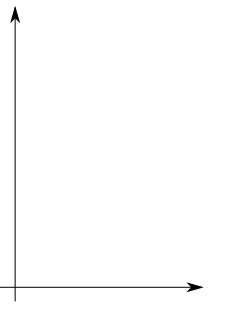
\includegraphics[width=0.35\textwidth]{regionexample1.svg}
%%     \caption{Example region 1}
%%     \label{regionexample1}
%%   \end{figure}
%% }{
  \begin{figure}[H]
    \centering
    \def\svgwidth{0.35\columnwidth}
    \input{figures/latex/regionexample1.pdf_tex}
    \caption{Example region 1}
    \label{regionexample1}
  \end{figure}
%% }

    \begin{align*}
      \int_0^1 \int_x^{2\sqrt{x}} yx^2 \, dy \, dx & = \int_0^1 \left[ \frac{y^2 x^2}{2} \right]_x^{2\sqrt{x}} \, dx = \int_0^1 x^3 - \frac{x^4}{2} \, dx  \\
      & = \left[ \frac{x^4}{4} - \frac{x^5}{10} \right]_0^1 = \frac{1}{4} - \frac{1}{10} = \frac{3}{20}.
    \end{align*}
    \item Some regions can be considered in either way -- especially those involving simple geometric shapes such as triangles.  In cases like this it may be that we can integrate in one order, but not the other.  In such situations, we may need to change the order of integration, as in the following integral.
    
    Calculate the double integral
      \[
        \int_0^2 \int_{x/2}^1 e^{y^2} \, dy \, dx.
      \]
    We cannot perform the $y$-integration first since we do not know an antiderivative of $e^{y^2}$.  Instead we will reverse the order of integration.  To find the new limits, we sketch the region of integration in figure (\ref{regionexample2}).
%% \nextalt{Request description from lecturer or tactile diagram.}
%% \iftoggle{web}
%% {
%%   \begin{figure}[H]
%%     \centering
%%     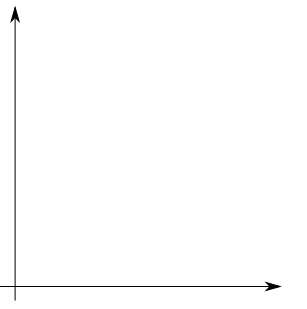
\includegraphics[width=0.4\textwidth]{regionexample4.svg}
%%     \caption{Example region 2}
%%     \label{regionexample2}
%%   \end{figure}
%% }{
  \begin{figure}[H]
    \centering
    \def\svgwidth{0.4\columnwidth}
    \input{figures/latex/regionexample4.pdf_tex}
    \caption{Example region 2}
    \label{regionexample2}
  \end{figure}
%% }

    In this region, $x$ varies from $0$ to the line $x = 2y$, and $y$ varies between $0$ and $1$.  Thus the integral is
      \begin{align*}
        \int_0^2 \int_{x/2}^1 e^{y^2} \, dy \, dx & = \int_0^1 \int_0^{2y} e^{y^2} \, dx \, dy  \\
        & = \int_0^1 \left[ xe^{y^2} \right]_0^{2y} \, dy  \\
        & = \int_0^1 2ye^{y^2} \, dy  \\
        & = \left[ e^{y^2} \right]_0^1 = e - 1.
      \end{align*}
    \end{enumerate}  
  \end{examples}



\subsection{Change of variable using the Jacobian}  \label{sect:Jacobian}

  Change of variable is the analogue of integration by substitution for double integrals.  It allows us to replace our variables $x$ and $y$ with new variables $u$ and $v$.  This can be useful for evaluating integrals over complicated regions.

  Suppose we want to evaluate the double integral of a function $f(x, y)$ over the region pictured in figure (\ref{regeval}).

%% \nextalt{Request description from lecturer or tactile diagram.}
%% \iftoggle{web}
%% {
%%  \begin{figure}[!htpb]
%%     \centering
%%     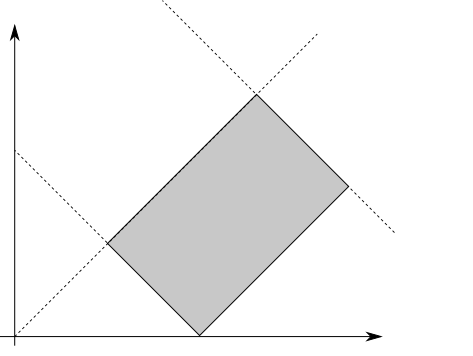
\includegraphics[width=0.6\textwidth]{JacobianRectanglexy.svg}
%%     \caption{Region of evaluation}
%%     \label{regeval}
%%   \end{figure}
%% }{
  \begin{figure}[!htpb]
    \centering
    \def\svgwidth{0.6\columnwidth}
    \input{figures/latex/JacobianRectanglexy.pdf_tex}
    \caption{Region of evaluation}
    \label{regeval}
  \end{figure}
%% }

  The region is rectangular, so integration ought to be easy -- but it's not because the sides of the rectangle are not parallel to the coordinate axes.  To evaluate this integral with the methods we already know we would need to divide the region into three subregions.
  % This is annoying/awkward.

  \emph{Solution:}  Draw some new axes!  We'll call them $u$ and $v$.  We want to choose them so that the region looks something like (figure (\ref{regnew})). 

%% \nextalt{Request description from lecturer or tactile diagram.}
%% \iftoggle{web}
%% {
%%   \begin{figure}[H]
%%     \centering
%%     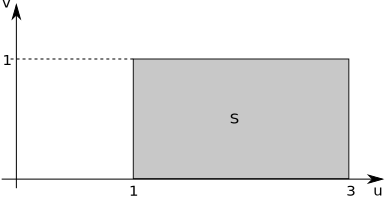
\includegraphics[width=0.6\textwidth]{JacobianRectangleuv.svg}
%%     \caption{Choose axes $u$ and $v$ to achieve this region}
%%     \label{regnew}
%%   \end{figure}
%% }{
  \begin{figure}[H]
    \centering
    \def\svgwidth{0.6\columnwidth}
    \input{figures/latex/JacobianRectangleuv.pdf_tex}
    \caption{Choose axes $u$ and $v$ to achieve this region}
    \label{regnew}
  \end{figure}
%% }

  How do we get from a point on the $(x, y)$-plane to the corresponding point on the $(u, v)$-plane?

  Define a \emph{transformation}
    \[
      U \colon \mathbb{R}^2 \longrightarrow \mathbb{R}^2
    \]
  where $U(x, y) = (u(x, y), v(x, y))$.

  To find $u$ and $v$ in terms of $x$ and $y$, we pick where we want our $u$- and $v$-axes to appear on the $(x, y)$-plane.

  $u$-axis: occurs when $v = 0$; should be parallel to the lines $y = x$ and $y = x - 1$, so pick
    \[
      v = x - y
    \]

  $v$-axis: occurs when $u = 0$; should be parallel to $y = 1 - x$ and $y = 3 - x$, so pick
    \[
      u = x + y
    \]

  So $U(x, y) = (x + y, x - y) = (u, v)$ takes a point on the $(x, y)$-plane, and gives a point on the $(u, v)$-plane.

  We want to use this to make a substitution that will turn
    \[
      \iint_R f(x, y) \, dA_{xy}
    \]
  (where $dA_{xy}$ is ``with respect to area on the $(x, y)$-plane'') into an integral in terms of $u$ and $v$, integrating over a region of the $(u, v)$-plane.

  \subsubsection*{Reminder: substitution for single integrals}

  If we have $x = g(u)$, then
    \[
      \int_a^b f(x) \, dx = \int_{g^{-1}(a)}^{g^{-1}(b)} f(g(u))g'(u) \, du.
    \]
  If $g$ is decreasing, $g'(u) < 0$, then $g^{-1}(b) < g^{-1}(a)$, so this is
    \begin{align*}
      \int_a^b f(x) \, dx & = - \int_{g^{-1}(b)}^{g^{-1}(a)} f(g(u))g'(u) \, du  \\
      & = \int_{g^{-1}(b)}^{g^{-1}(a)} f(g(u))\left|g'(u)\right| \, du.
    \end{align*}
  So in general,
    \[
      \int_a^b f(x) \, dx = \int_{\alpha}^{\beta} f(g(u))\left|g'(u)\right| \, du,
    \]
  where $\alpha$, $\beta$ are the $u$-limits, and $\alpha < \beta$.

  So we replace $dx$ with $\left|g'(u)\right|\, du$ (and swap the limits when $g'(u) < 0$).

  \subsubsection*{Change of variable for double integrals}

  For double integrals, we need to replace $dA_{x, y}$ (area on the $(x, y)$-plane) with something in terms of $dA_{uv}$ (area on the $(u, v)$-plane).  The expression we use is related to the derivatives of $x(u, v)$ and $y(u, v)$.

  \begin{definition}
    If $T \colon \mathbb{R}^2 \rightarrow \mathbb{R}^2$ is a transformation from the $(u, v)$-plane to the $(x, y)$-plane defined by
    \[
      x = x(u, v), \quad y - y(u, v),
    \]
    then the \emph{Jacobian of $T$}, denoted $\displaystyle{\frac{\partial(x, y)}{\partial(u, v)}}$ (or $J(u, v)$), is defined by
    \[
      \frac{\partial(x, y)}{\partial(u, v)} = \left|
      \begin{matrix}
        \dfrac{\strut\partial x}{\strut\partial u} & \dfrac{\strut\partial x}{\strut\partial v}  \\
        \dfrac{\strut\partial y}{\strut\partial u} & \dfrac{\strut\partial y}{\strut\partial v}
      \end{matrix}
      \right| = \frac{\partial x}{\partial u}\frac{\partial y}{\partial v} - \frac{\partial y}{\partial u}\frac{\partial x}{\partial v}.
    \]
  \end{definition}

  The Jacobian (named after 19th Century German mathematician Carl Jacobi) appears in place of $g'(u)$ in the change of variables formula.

  \begin{theorem}
    If the transformation $x = x(u, v)$, $y = y(u, v)$ maps the region $S$ in the $(u, v)$-plane to $R$ in the $(x, y)$-plane, and if $\displaystyle{\frac{\strut\partial(x, y)}{\strut\partial(u, v)}} \neq 0$ and does not change sign on $S$, then
      \[
        \iint_R f(x, y) \, dA_{xy} = \iint_S f(x(u, v), y(u, v)) \left|\displaystyle{\frac{\partial(x, y)}{\partial(u, v)}}\right| \, dA_{uv}.
      \]
  \end{theorem}

  \begin{example}
    We now use this to evaluate an integral over the rectangular region from the beginning of the section.  Consider
      \[
        \iint_R \frac{x - y}{x + y} \, dA_{xy},
      \]
    where $R$ is the rectangular region with vertices
      \[
        (1, 0), \quad \left(\frac{1}{2}, \frac{1}{2}\right), \quad \left(\frac{3}{2}, \frac{3}{2}\right), \quad (2, 1),
      \]
    as described at the beginning of the section.

    For our transformation from the $(x, y)$-plane to the $(u, v)$-plane, we chose
      \[
        u = x + y, \quad v = x - y.
      \]
    To find the Jacobian, we need to find $x$ and $y$ in terms of $u$ and $v$.
      \[
        u + v = x + y + x - y = 2x \implies x = \frac{u + v}{2},
      \]
      \[
        u - v = x + y - x + y = 2y \implies y = \frac{u - v}{2}.
      \]
    Hence
      \[
        \frac{\partial x}{\partial u} = \frac{1}{2}, \quad \frac{\partial x}{\partial v} = \frac{1}{2}, \quad \frac{\partial u}{\partial u} = \frac{1}{2}, \quad \frac{\partial y}{\partial v} = - \frac{1}{2},
      \]
    so the Jacobian is
      \[
        \left|
        \begin{matrix}
          \dfrac{\strut 1}{\strut 2} & \dfrac{\strut 1}{\strut 2}  \\
          \dfrac{\strut 1}{\strut 2} & - \dfrac{\strut 1}{\strut 2}
        \end{matrix}
        \right| = \frac{1}{2} \times \left(- \frac{1}{2}\right) - \frac{1}{2} \times \frac{1}{2} = - \frac{1}{4} - \frac{1}{4} = - \frac{1}{2}.
      \]
    So
      \begin{align*}
        \iint_R \frac{x - y}{x + y} \, dA_{xy} & = \iint_S \frac{v}{u} \times \left|- \frac{1}{2}\right| \, dA_{uv}  \\
        & = \int_0^1 \int_1^3 \frac{1}{2}\frac{v}{u} \, du \, dv  \\
        & = \frac{1}{2} \int_0^1 \left[v\ln\left|u\right|\right]_1^3 \, dv  \\
        & = \frac{1}{2}\ln(3)\int_0^1 v \, dv  \\
        & = \frac{1}{2}\ln(3)\left[\frac{1}{2}v^2\right]_0^1  \\
        & = \frac{1}{4}\ln(3).
      \end{align*}
  \end{example}

  Change of variable doesn't just work for rectangular regions -- with the right choice of variable, we can apply it to other regions as well, and even transform non-rectangular regions into rectangular ones.

  \begin{example}
    Evaluate
      \[
        \iint_R e^{xy} \, dA
      \]
    where $R$ is the region bounded by the lines
      \[
        y = \frac{1}{2}x, \quad y = x,
      \]
    and the hyperbolas
      \[
        y = \frac{1}{x}, \quad y = \frac{2}{x}.
      \]
 
%% \nextalt{Request description from lecturer or tactile diagram.}
%% \iftoggle{web}
%% {
%%   \begin{figure}[H]
%%     \centering
%%     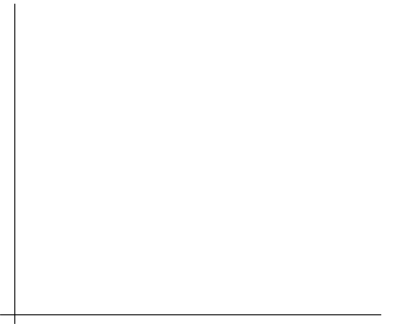
\includegraphics[width=0.6\textwidth]{JacobianHyperbolae.svg}
%%     \caption{Sketch of region}    
%%     \label{JacobianHyperbolae}
%%   \end{figure}
%% }{
  \begin{figure}[H]
    \centering
    \def\svgwidth{0.6\columnwidth}
    \input{figures/latex/JacobianHyperbolae.pdf_tex}
    \caption{Sketch of region}    
    \label{JacobianHyperbolae}
  \end{figure}
%% }

    We want a transformation that will change this region (figure (\ref{JacobianHyperbolae})) into a rectangle in the $(u, v)$-plane, so the boundary curves should correspond to constant values of $u$ and $v$.

    Rewrite the boundary curves as
      \[
        \frac{y}{x} = \frac{1}{2}, \quad \frac{y}{x} = 1, \quad xy = 1, \quad xy = 2.
      \]
    So try the transformation
      \[
        u = \frac{y}{x}, \quad v = xy.
      \]
    The lines in the $(u, v)$-plane corresponding to the boundary curves in the $(x, y)$-plane are
      \[
        u = \frac{1}{2}, \quad u = 1, \quad v = 1, \quad v = 2.
      \]
    This gives us our $u$-limits and $v$-limits.

    For the Jacobian, we need to express $x$ and $y$ in terms of $u$ and $v$:
      \[
        uv = \frac{y}{x} \times xy = y^2 \implies y = \sqrt{uv}
      \]
      \[
        \frac{v}{u} = xy \times \frac{x}{y} = x^2 \implies x = \sqrt{\frac{v}{u}}
      \]
    ($x$, $y$, $u$, $v$ are all positive on the region, so we can safely use the positive square roots)

    So the Jacobian is:
    \[
      \frac{\partial(x, y)}{\partial(u, v)} = \left|
      \begin{matrix}
        \dfrac{\strut\partial x}{\strut\partial u} & \dfrac{\strut\partial x}{\strut\partial v}  \\
        \dfrac{\strut\partial y}{\strut\partial u} & \dfrac{\strut\partial y}{\strut\partial v}
      \end{matrix}
      \right| =
      \left|
      \begin{matrix}
        - \dfrac{1}{2u}\sqrt{\dfrac{v}{u}} & \dfrac{1}{2\sqrt{uv}}  \\
        \dfrac{1}{2}\sqrt{\dfrac{v}{u}} & \dfrac{1}{2}\sqrt{\dfrac{u}{v}}
      \end{matrix}
      \right| = - \frac{1}{4u} - \frac{1}{4u} = - \frac{1}{2u}.
    \]
    Observe that, unlike in the previous example, this Jacobian is not constant.

     Thus the integral is
       \begin{align*}
         \iint_R e^{xy} \, dA_{xy} & = \iint_S e^v \left|-\frac{1}{2u}\right| \, dA_{uv}  \\
         & = \frac{1}{2} \iint_S \frac{1}{u}e^v \, dA_{uv}  \\
         & = \frac{1}{2} \int_1^2 \int_{1/2}^1 \frac{1}{u}e^v \, du \, dv  \\
         & = \frac{1}{2} \int_1^2 \left[e^v\ln\left|u\right|\right]_{1/2}^1 \, dv  \\
         & = \frac{1}{2}\ln(2)\int_1^2 e^v \, dv  \\
         & = \frac{1}{2}(e^2 - e)\ln(2).
       \end{align*}
  \end{example}



\subsection{Polar coordinates}

  In Section~\ref{sect:Jacobian} we saw that, for integrals over certain awkward-shaped regions, it is convenient to be able to transform the plane to a new set of coordinate axes.

  In the examples we've seen so far this transformation gave us a new cartesian plane.  In this section we look at a different coordinate system: \emph{polar coordinates}.

  \subsubsection*{Cartesian coordinates:}

  \begin{itemize}
    \item Two perpendicular axes (figure (\ref{cartesian})).
    \item Specify a point on the plane using two real numbers, $x$ and $y$ -- horizontal and vertical distances from origin.
    \item Each point $P$ has unique $(x, y)$-coordinates.
    \item Named after Ren\'e Descartes.  Also known as rectangular coordinates.
  \end{itemize}

%% \nextalt{Request description from lecturer or tactile diagram.}
%% \iftoggle{web}
%% {
%%   \begin{figure}[H]
%%     \centering
%%     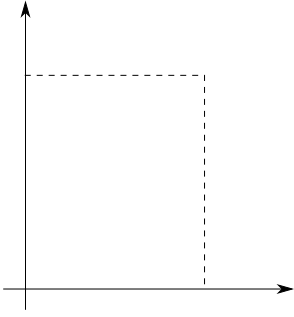
\includegraphics[width=0.3\textwidth]{cartesian.svg}
%%     \caption{Cartesian coordinates}
%%     \label{cartesian}
%%   \end{figure}
%% }{
  \begin{figure}[H]
    \centering
    \def\svgwidth{0.3\columnwidth}
    \input{figures/latex/cartesian.pdf_tex}
    \caption{Cartesian coordinates}
    \label{cartesian}
  \end{figure}
%% }


  \subsubsection*{Polar coordinates:}

%% \nextalt{Request description from lecturer or tactile diagram.}
%% \iftoggle{web}
%% {
%%   \begin{figure}[H]
%%     \centering
%%     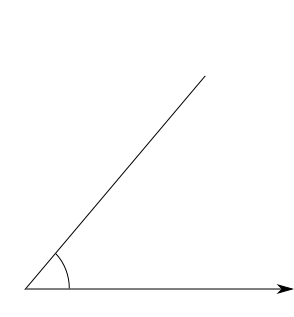
\includegraphics[width=0.29\textwidth]{polar.svg}
%%     \caption{Polar coordinates}
%%     \label{polar}
%%   \end{figure}
%% }{
  \begin{figure}[H]
    \centering
    \def\svgwidth{0.29\columnwidth}
    \input{figures/latex/polar.pdf_tex}
    \caption{Polar coordinates}
    \label{polar}
  \end{figure}
%% }

  \begin{itemize}
    \item One axis (``polar axis'') -- like positive half of the cartesian $x$-axis, with origin $O$ (figure (\ref{polar})).
    \item Specify a point $P$ by two real numbers:
      \begin{itemize}
        \item $r$ (``radius''): distance from the origin;
        \item $\theta$ : anticlockwise angle between axis and line segment from $O$ to $P$.
      \end{itemize}
    \item For a given $P$, $r$ is unique, but $\theta$ is not, since:
      \[
        (r, \theta) = (r, \theta + 2k\pi), \quad k \in \mathbb{Z}.
      \]
    \item $(0, \theta)$ is the origin for all values of $\theta$.
  \end{itemize}

  \subsubsection*{Relationship between polar and cartesian coordinates}

  We can move between polar and cartesian coordinates.  Consider figure (\ref{polarcartesian}).
%% \nextalt{Request description from lecturer or tactile diagram.}
%% \iftoggle{web}
%% {
%%   \begin{figure}[H]
%%     \centering
%%     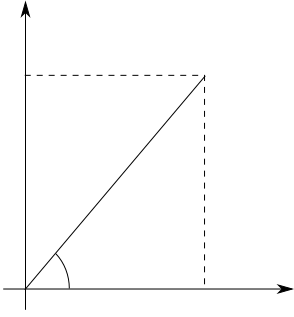
\includegraphics[width=0.29\textwidth]{polarcartesian.svg}
%%     \caption{Triangle with vertices $(0, 0)$, $(x, 0)$, $(x, y)$}
%%     \label{polarcartesian}
%%   \end{figure}
%% }{
  \begin{figure}[H]
    \centering
    \def\svgwidth{0.29\columnwidth}
    \input{figures/latex/polarcartesian.pdf_tex}
    \caption{Triangle with vertices $(0, 0)$, $(x, 0)$, $(x, y)$}
    \label{polarcartesian}
  \end{figure}
%% }

  Considering the triangle with vertices $(0, 0)$, $(x, 0)$, $(x, y)$, we observe that
    \[
      \cos(\theta) = \frac{x}{r}, \quad \sin(\theta) = \frac{y}{r},
    \]
  so to change from polar to cartesian coordinates, use the transformation
    \[
      x = r\cos(\theta), \quad y = r\sin(\theta).
    \]

  Changing from cartesian to polar coordinates is a bit trickier.  By Pythagoras' Theorem:
    \[
      r^2 = x^2 + y^2.
    \]
  There is no easy formula for $\theta$, but we can use
    \[
      \tan(\theta) = \frac{y}{x}.
    \]
  Note that $\arctan$ gives values between $-\dfrac{\pi}{2}$ and $\dfrac{\pi}{2}$, so $\arctan$ will not consistently give the value of $\theta$.

  \subsubsection*{Equations of curves in polar coordinates}
  % NOTE: I'm leaving this in the notes for now, though I may cut it from the lectures if I am running low on time -- which is likely given last year's timings.

  Some curves are much easier to write in polar coordinates than in cartesian coordinates.

  \begin{examples}
    \begin{enumerate}
      \item Circle of radius $a$.
        
        In cartesian coordinates:
          \[
            x^2 + y^2 = a^2,
          \]
        or
          \[
            y = \sqrt{a^2 - x^2}, \quad y = - \sqrt{a^2 - x^2}.
          \]
        In polar coordinates:
          \[
            r = a.
          \]
        This will be very useful for simplifying integrals over circular regions.
      \item Spirals: Archimedean spiral (figure (\ref{arch})), $r = a\theta$, $a$ constant and Logarithmic spiral (figure (\ref{log})), $r = ae^{b\theta}$, $a$, $b$ constant.

        %% \nextalt{Request description from lecturer or tactile diagram.}
        \begin{figure}[!htbp]
          \centering
          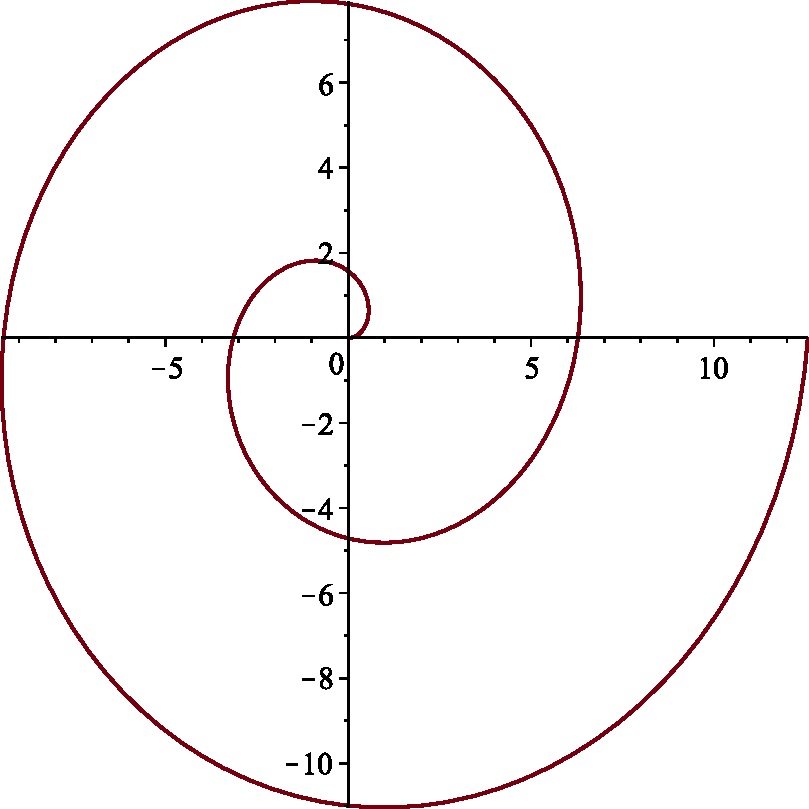
\includegraphics[width=0.5\textwidth]{archspiral.pdf}
          \caption{Archimedean spiral}
          \label{arch}
        \end{figure}

        %% \nextalt{Request description from lecturer or tactile diagram.}
        \begin{figure}[!hbtp]
          \centering
          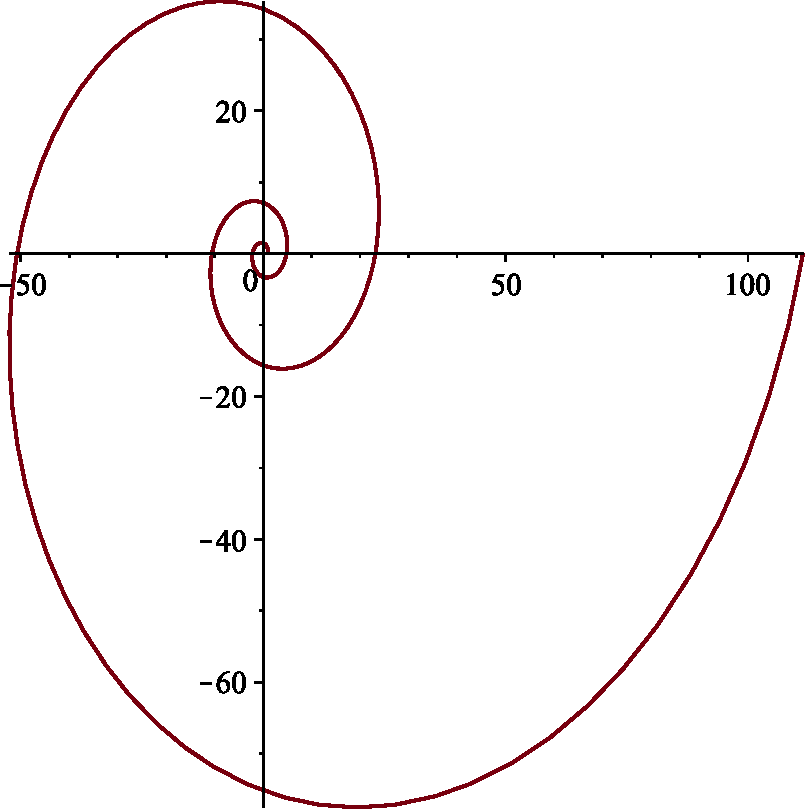
\includegraphics[width=0.5\textwidth]{logspiral.pdf}
          \caption{Logarithmic spiral}
          \label{log}
        \end{figure}
        
      \item Cardioids (figure (\ref{card})): $r = a \pm a\sin(\theta)$ and $a \pm a\cos(\theta)$, $a$ constant.

        %% \nextalt{Request description from lecturer or tactile diagram.}
        \begin{figure}[!htpb]
          \centering
          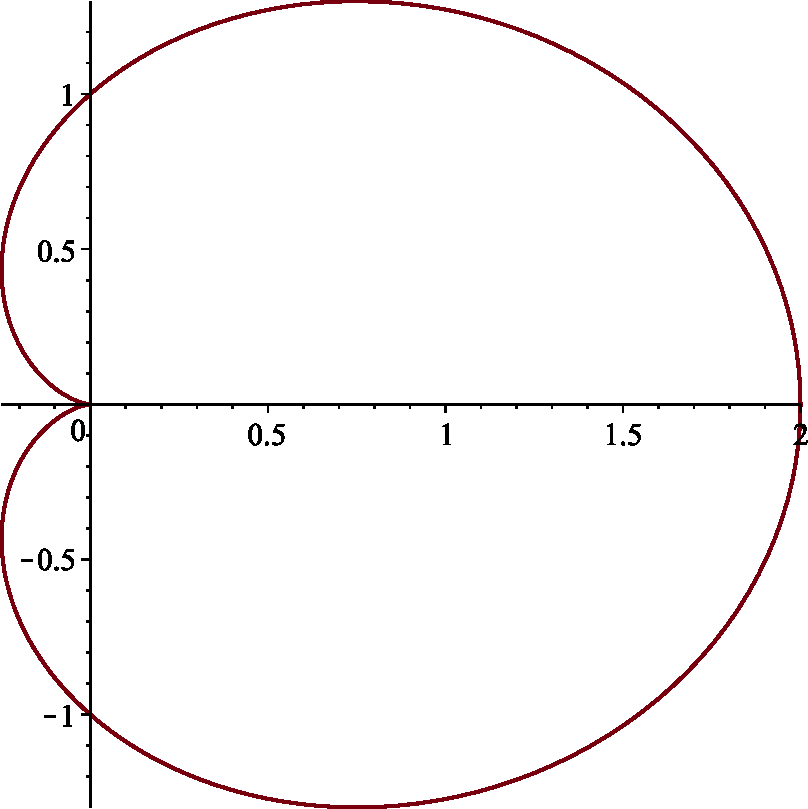
\includegraphics[width=0.5\textwidth]{cardioid.pdf}
          \caption{Cardioid}
          \label{card}
        \end{figure}

        More generally: lima\c{c}ons $r = a \pm b\sin(\theta)$, $r = a \pm b\cos(\theta)$, $a$, $b$ constants.
    \end{enumerate}
  \end{examples}
  
  \subsubsection*{Simple polar regions}
  
  When we use polar coordinates for integration, we will integrate over a particular kind of region that is straightforward to express in polar coordinates, called a \emph{simple polar region}.
  
  \begin{definition}
    A \emph{simple polar region} is a region of the plane enclosed between two \emph{rays} $\theta = \alpha$, $\theta = \beta$, and two (continuous) curves $r = r_1(\theta)$, $r = r_2(\theta)$, satisfying
    \[
      \alpha \leq \beta, \quad \beta - \alpha \leq 2\pi, \quad 0 \leq r_1(\theta) \leq r_2(\theta).
    \]
  \end{definition}
  
  An example is shown in the diagram (\ref{simplepolarregion}).
  
%% \nextalt{Request description from lecturer or tactile diagram.}
%% \iftoggle{web}
%% {
%%   \begin{figure}[H]
%%     \centering
%%     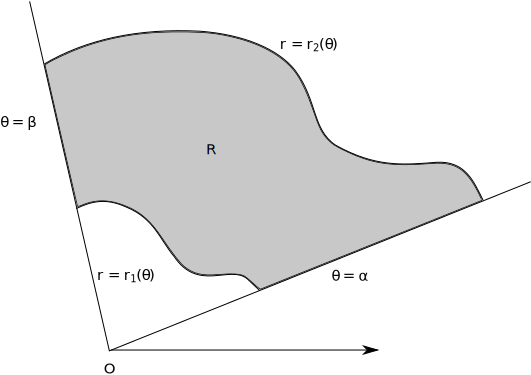
\includegraphics[width=0.7\textwidth]{simplepolarregion.svg}
%%     \caption{A simple polar region}
%%     \label{simplepolarregion}
%%   \end{figure}
%% }{
  \begin{figure}[H]
    \centering
    \def\svgwidth{0.7\columnwidth}
    \input{figures/latex/simplepolarregion.pdf_tex}
    \caption{A simple polar region}
    \label{simplepolarregion}
  \end{figure}
%% }


\subsection{Double integrals in polar coordinates}

  Using change of variable and the Jacobian, we can convert an integral in cartesian coordinates into an integral in polar coordinates.  This can simplify certain integrals, especially those over circular regions, and those involving $x^2 + y^2$.

  \begin{example}[Volume of a sphere]
    In cartesian coordinates, a sphere of radius $a$ has the equation
      \[
        x^2 + y^2 + z^2 = a^2,
      \]
    or:
      \[
        \text{upper hemisphere: } z = \sqrt{a^2 - x^2 - y^2},
      \]
      \[
        \text{lower hemisphere: } z = - \sqrt{a^2 - x^2 - y^2}.
      \]
    So the volume of the sphere is
      \[
        V = 2\iint_R \sqrt{a^2 - x^2 - y^2} \, dA,
      \]
    where $R$ is the circular region bounded by
      \[
        x^2 + y^2 = a^2.
      \]
    Thus in cartesian coordinates, the integral is:
      \[
        V = 2\int\nolimits_{-a}^a \int\nolimits_{-\sqrt{a^2 - x^2}}^{\sqrt{a^2 - x^2}} \sqrt{a^2 - x^2 - y^2} \, dy \, dx.
      \]
    This is complicated.  We can simplify it by changing to polar coordinates.  We have
      \[
        x = r\cos(\theta), \quad y = r\sin(\theta),
      \]
    so the Jacobian is
    \[
      \frac{\partial(x, y)}{\partial(r, \theta)} = \left|
      \begin{matrix}
        \dfrac{\strut\partial x}{\strut\partial r} & \dfrac{\strut\partial x}{\strut\partial \theta}  \\
        \dfrac{\strut\partial y}{\strut\partial r} & \dfrac{\strut\partial y}{\strut\partial \theta}
      \end{matrix}
      \right| =
      \left|
      \begin{matrix}
        \cos(\theta) & -r\sin(\theta)  \\
        \sin(\theta) & r\cos(\theta)
      \end{matrix}
      \right| = r\cos^2(\theta) + r\sin^2(\theta) = r.
    \]
    Note that the region $R$ is a simple polar region; the boundary rays and curves give the following limits for the integral:
      \[
        0 \leq \theta \leq 2\pi,
      \]    
      \[
        0 \leq r \leq a.
      \]
    Thus the volume is
      \begin{align*}
        V & = 2\int_0^{2\pi} \int_0^a r\sqrt{a^2 - r^2} \, dr \, d\theta  \\
        & = \int_0^{2\pi} \left[-\frac{2}{3} (a^2 - r^2)^{3/2}\right]_0^a \, d\theta  \\
        & = \int_0^{2\pi} \left(-\frac{2}{3}(a^2 - a^2)^{3/2} + \frac{2}{3}(a^2 - 0^2)^{3/2}\right) \, d\theta  \\
        & = \int_0^{2\pi} \frac{2}{3}a^3 d\theta  \\
        & = \left[\frac{2}{3}a^3\theta\right]_0^{2\pi}  \\
        & = \frac{4}{3}\pi a^3.
      \end{align*}
    This agrees with the standard formula for the volume of a sphere.
  \end{example}

  In this example we started with the integrand and limits in cartesian coordinates, and converted to polar coordinates, using the Jacobian to change variable.  However, we may be given the integrand and limits in polar form originally.  In this case, although we don't need to make a change of variable, we still need to multiply the integrand by the Jacobian.

  \begin{theorem}
    If $R$ is a simple polar region bounded by the rays $\theta = \alpha$, $\theta = \beta$, and the curves $r = r_1(\theta)$, $r = r_2(\theta)$, and if $f(r, \theta)$ is continuous on $R$, then
      \[
        \iint_R f(r,\theta) \, dA = \int_{\alpha}^{\beta} \int_{r_1(\theta)}^{r_2(\theta)} f(r, \theta) r \, dr \, d\theta.
      \]
  \end{theorem}

  We won't prove this theorem, but here is an explanation of why it is true:

  Double integration treats regions with constant limits as rectangles, but in polar coordinates such regions are not rectangular.  Consider, for example figure (\ref{notrectangles}).
  
%% \nextalt{Request description from lecturer or tactile diagram.}
%% \iftoggle{web}
%% {
%%   \begin{figure}[H]
%%     \centering
%%     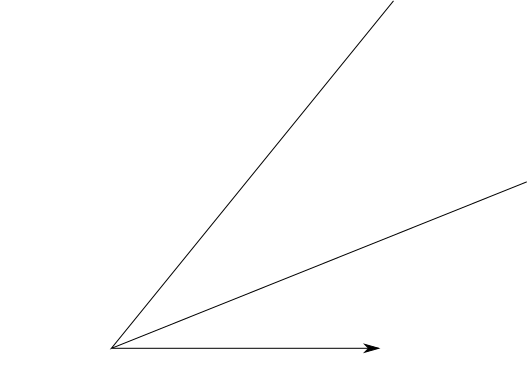
\includegraphics[width=0.55\textwidth]{notrectangles.svg}
%%     \caption{Region which is not rectangular}
%%     \label{notrectangles}
%%   \end{figure}
%% }{
  \begin{figure}[H]
    \centering
    \def\svgwidth{0.55\columnwidth}
    \input{figures/latex/notrectangles.pdf_tex}
    \caption{Region which is not rectangular}
    \label{notrectangles}
  \end{figure}
%% }
  
  Double integration treats the regions $R_1$ and $R_2$ as rectangles with the same area -- but they're not rectangles, and $R_2$ is much larger than $R_1$.  The contribution made to the area of a region is proportional to the distance from the origin (i.e. proportional to the radius).  This explains why the Jacobian is $r$.
  
  When we use double integration to integrate something in polar form, we are effectively changing variable to a cartesian $(r, \theta)$-plane.  Note that $r$ is always positive, and $\theta$ is between $0$ and $2\pi$, but that otherwise this is a standard cartesian plane and that regions with constant limits are now rectangular.

  \begin{example}
    Evaluate the double integral
      \[
        \iint_R \sin(\theta) \, dA,
      \]
    where $R$ is the region in the first quadrant between the the circle $r = 2$ and the cardioid $r = 2 + 2\cos(\theta)$ (figure (\ref{cardioidcircle})).
    
%% \nextalt{Request description from lecturer or tactile diagram.}
%% \iftoggle{web}
%% {
%%   \begin{figure}[H]
%%     \centering
%%     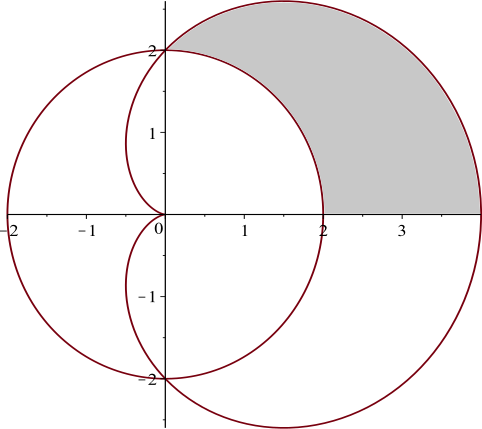
\includegraphics[width=0.5\textwidth]{cardioidcircle.svg}
%%     \caption{Region $R$}
%%     \label{cardioidcircle}
%%   \end{figure}
%% }{  
  \begin{figure}[H]
    \centering
    \def\svgwidth{0.5\columnwidth}
    \input{figures/latex/cardioidcircle.pdf_tex}
    \caption{Region $R$}
    \label{cardioidcircle}
  \end{figure}
%% }
  
    Observe that $R$ is a simple polar region, with limits given by
      \[
        0 \leq \theta \leq \frac{\pi}{2},
      \]
      \[
        2 \leq r \leq 2 + 2\cos(\theta).
      \]
    Thus the integral is
      \begin{align*}
        \iint_R \sin(\theta) \, dA & = \int\nolimits_0^{\pi/2} \int\nolimits_2^{2 + 2\cos(\theta)} \sin(\theta)r \, dr \, d\theta  \\
        & = \int_0^{\pi/2} \left[\frac{1}{2}r^2\sin(\theta)\right]_2^{2 + 2\cos(\theta)} \, d\theta  \\
        & = 2\int_0^{\pi/2} (1 + \cos(\theta))^2 \sin(\theta) - \sin(\theta) \, d\theta  \\
        & = 2\left[-\frac{1}{3}(1 + \cos(\theta))^3 + \cos(\theta)\right]_0^{\pi/2}  \\
        & = 2\left(-\frac{1}{3}-\left(-\frac{5}{3}\right)\right)  \\
        & = \frac{8}{3}.
      \end{align*}
  \end{example}
  
  
  
\subsection{Triple integrals}

  As with partial differentiation, we can extend double integration to higher numbers of variables.  We will look at integration in the $3$ variable case (we won't go any higher than this).

  \subsubsection*{$3$-dimensional regions}

  \emph{Double integrals:} integrate over a $2$D region of the $(x, y)$-plane.

  \emph{Triple integrals:} integrate over a $3$D region of $(x, y, z)$-space.

  For us, this will always be a finite solid.

  \emph{Notation}

  The triple integral of a function of $3$ variables, $f(x, y, z)$, over a $3$-dimensional region $G$ is denoted
    \[
      \iiint_G f(x, y, z) \, dV.
    \]
  You should read $dV$ as ``with respect to volume''.  The $G$ doesn't stand for anything -- unlike the case of double-integrals (where we use $R$) there is no standard letter used for $3$D regions.
  % I have followed Anton et al.

  \subsubsection*{What does it respresent?}

  In the $1$ and $2$ variable cases, definite integrals represented a tangible geometric quantity.

  \emph{Single integrals:} area under a curve.

  \emph{Double integrals:} volume under a surface.

  \emph{Triple integrals:} ?

  We live in a universe with $3$ spacial dimensions, but a triple integral is something $4$-dimensional, so we don't have the words to describe what it represents geometrically.

  Triple integrals can tell us about physical quantities though.  For example:
    \begin{itemize}
      \item mass of an object (integrate its density)
      \item centre of mass/centre of gravity
      \item volume
      \item gravitational potential
      \item magnetic and electric fields
      \item position of a particle in quantum physics
    \end{itemize}

  \subsubsection*{Properties of triple integrals}

  As with single and double integrals, we have the usual linearity properties:
    \begin{itemize}
      \item For a constant $c$,
    \[
      \iiint_G cf(x, y, z) \, dV = c\iiint_G f(x, y, z) \, dV;
    \]
      \item For functions $f(x, y, z)$ and $g(x, y, z)$,
    \[
      \iiint_G f(x, y, z) + g(x, y, z) \, dV = \iiint_G f(x, y, z)\, dV + \iiint_G g(x, y, z) \, dV.
    \]
    \end{itemize}

  Also, if the region $G$ can be subdivided into regions $G_1$ and $G_2$, then
    \[
      \iiint_G f(x, y, z) \, dV = \iiint_{G_1} f(x, y, z) \, dV + \iiint_{G_2} f(x, y, z) \, dV.
    \]

  \subsubsection*{Triple integrals over cuboids}

  For double integrals, the simplest regions for integration were rectangular boxes.

  Similarly, for triple integration, the simplest regions are cuboids -- like the case of evaluating double integrals over rectangles, triple integrals over cuboids have constant limits.

  \begin{theorem}
    Let $G$ be the cuboid defined by
      \[
        a \leq x \leq b, \quad c \leq y \leq d, \quad k \leq z \leq l.
      \]
    If $f(x, y, z)$ is continuous on the region $G$, then
      \[
        \iiint_G f(x, y, z) \, dV = \int_a^b \int_c^d \int_k^l f(x, y, z) \, dz \, dy \, dx.
      \]
    Moreover, in the integral on the right, one can alter the order of integration, without changing the resulting value of the integral.
  \end{theorem}

  For triple integrals, there are six possible orders of integration.  In the following example we will evaluate a triple integral using one of these orders, but any other order would give the same result.

  \begin{example}
    Evaluate the triple integral
      \[
        \iiint_G 6x^3y^2z \, dV
      \]
    over the cuboid $G$ defined by
      \[
        1 \leq x \leq 2, \quad -1 \leq y \leq 1, \quad 0 \leq z \leq 2.
      \]

      \begin{align*}
        \iiint_G 6x^3y^2z \, dV & = \int_1^2 \int_{-1}^1 \int_0^2 6x^3y^2z \, dz \, dy \, dx  \\
        & = \int_1^2 \int_{-1}^1 \left[3x^3y^2z^2\right]_0^2 \, dy \, dx  \\
        & = \int_1^2 \int_{-1}^1 12x^3y^2 \, dy \, dx  \\
        & = \int_1^2 \left[4x^3y^3\right]_{-1}^1 \, dx  \\
        & = \int_1^2 8x^3 \, dx  \\
        & = \left[2x^4\right]_1^2 = 2 \times 16 - 2 = 30.
      \end{align*}
  \end{example}

  \subsubsection*{More general regions}

  In the $2$-variable case we looked at regions of the form in figure (\ref{typeiregion2}).
%% \nextalt{Request description from lecturer or tactile diagram.}
%% \iftoggle{web}
%% {
%%   \begin{figure}[H]
%%     \centering
%%     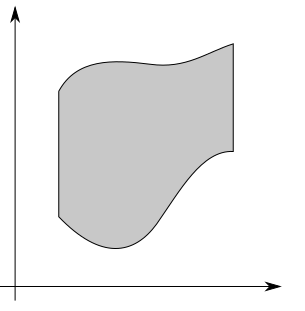
\includegraphics[width=0.45\textwidth]{typeiregion.svg}
%%     \caption{Type I region}
%%     \label{typeiregion2}
%%   \end{figure}
%% }{
  \begin{figure}[H]
    \centering
    \def\svgwidth{0.45\columnwidth}
    \input{figures/latex/typeiregion.pdf_tex}
    \caption{Type I region}
    \label{typeiregion2}
  \end{figure}
%% }

  In the $3$-variable case, we generalise this by replacing
    \begin{itemize}
      \item $[a, b]$ with a region $R$ of the $(x, y)$-plane (one we can perform double integration over);
      \item the curves $y = g_1(x)$ and $y=g_2(x)$ with surfaces $z = g_1(x, y)$ and $z = g_2(x, y)$.
    \end{itemize}

  This gives regions $G$ of the form shown in figure (\ref{tripleform}).
%% \nextalt{Request description from lecturer or 3D object.}
%% \iftoggle{web}
%% {
%%   \begin{figure}[!htbp]
%%     \centering
%%     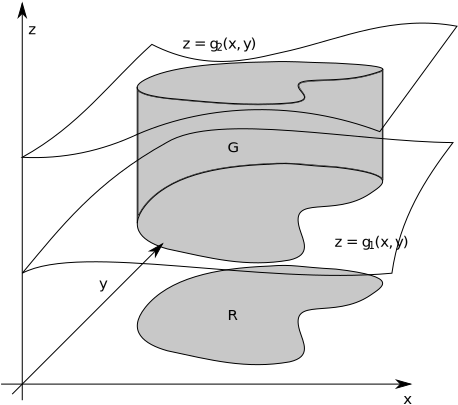
\includegraphics[width=0.63\textwidth]{tripleintegral3dregion.svg}
%%     \caption{Form of regions}
%%     \label{tripleform}
%%   \end{figure}
%% }{
  \begin{figure}[!htbp]
    \centering
    \def\svgwidth{0.63\columnwidth}
    \input{figures/latex/tripleintegral3dregion.pdf_tex}
    \caption{Form of regions}
    \label{tripleform}
  \end{figure}
%% }

  \emph{Terminology:}
    \begin{itemize}[topsep=0pt]
      \item $G$ is called a \emph{simple $xy$-solid};
      \item $z = g_1(x, y)$ is the \emph{lower surface};
      \item $z = g_2(x, y)$ is the \emph{upper surface}.
    \end{itemize}

  \begin{theorem}
    For a simple $xy$-solid $G$, as described above, and $f(x, y, z)$ continuous on $G$,
      \[
        \iiint_G f(x, y, z) \, dV = \iint_R \left[\int_{g_1(x, y)}^{g_2(x, y)} f(x, y, z) \, dz \right] \, dA.
      \]
  \end{theorem}

  \begin{example}
    Evaluate the triple integral
      \[
        \iiint_G z \, dV.
      \]
    where $G$ is the simple $xy$-solid bounded by
      \[
        g_1(x, y) = -\sqrt{1 - y^2}, \quad g_2(x, y) = \sqrt{1 - y^2},
      \]
    and the projection of $G$ onto the $(x, y)$-plane is the triangle (figure (\ref{tripleregionxyplane})) with vertices
      \[
        (0, 0), \quad (0, 1), \quad (1, 1).
      \]
%% \nextalt{Request description from lecturer or tactile diagram.}
%% \iftoggle{web}
%% {
%%   \begin{figure}[H]
%%     \centering
%%     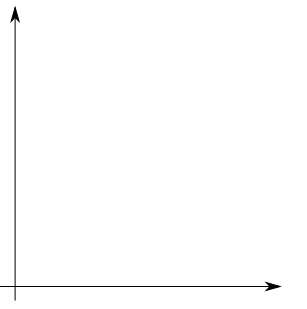
\includegraphics[width=0.32\textwidth]{tripleregionxyplane.svg}
%%     \caption{Projection of $G$ onto the $(x,y)$-plane}
%%     \label{tripleregionxyplane}
%%   \end{figure}
%% }{
  \begin{figure}[H]
    \centering
    \def\svgwidth{0.32\columnwidth}
    \input{figures/latex/tripleregionxyplane.pdf_tex}
    \caption{Projection of $G$ onto the $(x,y)$-plane}
    \label{tripleregionxyplane}
  \end{figure}
%% }

    From the diagram, we have
      \begin{itemize}[topsep=0pt]
        \item $y$-limits: $x$ and $1$;
        \item $x$-limits: $0$ and $1$.
      \end{itemize}
    Thus the integral is
      \begin{align*}
        \iiint_G z \, dV & = \int_0^1 \int_x^1 \int_{-\sqrt{1 - y^2}}^{\sqrt{1 - y^2}} z \, dz \, dy \, dx  \\
        & = \int_0^1 \int_x^1 \left[\frac{1}{2}z\right]_{-\sqrt{1 - y^2}}^{\sqrt{1 - y^2}} \, dy \, dx  \\
        & = \int_0^1 \int_x^1 1 - y^2 \, dy \, dx  \\
        & = \int_0^1 \left[y - \frac{y^3}{3}\right]_x^1 \, dx  \\
        & = \int_0^1 1 - \frac{1}{3} - x + \frac{x^3}{3} \, dx  \\
        & = \int_0^1 \frac{x^3}{3} - x + \frac{2}{3} \, dx  \\
        & = \left[\frac{x^4}{12} - \frac{x^2}{2} + \frac{2}{3}x\right]_0^1  \\
        & = \frac{1}{12} - \frac{1}{2} + \frac{2}{3}  \\
        & = \frac{1}{4}.
      \end{align*}
  \end{example}  




\subsection{Triple integrals in spherical coordinates}
  
  % ``a lot'' too colloquial?
  % This was written in 30 seconds and needs rewording.  I will not write it out in the lecture anyway.
  There are a lot of possibilities for three-dimensional regions, and so far we can only integrate over a very narrow range of possibilities.  In order to expand our possibilities for regions to integrate over, we will use an alternative coordinate system called \emph{spherical coordinates}.

  Spherical coordinates are a $3$-dimensional analogue of polar coordinates (figure (\ref{spherical})).  In this case we have three coordinates:
    \begin{itemize}
      \item radius $r$ (sometimes denoted $\rho$), the distance from the origin;
      \item $\theta$, the angle from the positive $x$-axis (called the \emph{azimuthal} angle);
      \item $\varphi$, the angle from the positive $z$-axis (called the \emph{polar} angle).
    \end{itemize}
  
%% \nextalt{Request description from lecturer or 3D object.}
%% \iftoggle{web}
%% {
%%   \begin{figure}[H]
%%     \centering
%%     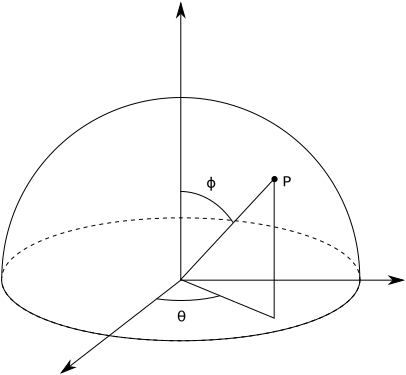
\includegraphics[width=0.5\textwidth]{spherical.svg}
%%     \caption{Spherical coordinates}
%%     \label{spherical}
%%   \end{figure}
%% }{
  \begin{figure}[H]
    \centering
    \def\svgwidth{0.5\columnwidth}
    \input{figures/latex/spherical.pdf_tex}
    \caption{Spherical coordinates}
    \label{spherical}
  \end{figure}
%% }
    
  \subsubsection*{Converting between spherical and cartesian coordinates}
  
  As in the two dimensional case with polar coordinates, we can convert between the spherical and cartesian coordinate systems.
  
  To convert from spherical to cartesian coordinates, use:
    \begin{align*}
      x & = r\sin(\varphi)\cos(\theta),  \\
      y & = r\sin(\varphi)\sin(\theta),  \\
      z & = r\cos(\varphi).
    \end{align*}
  As for polar coordinates, these can all be derived geometrically by considering the appropriate right-angled triangles.
  
  To convert from cartesian to spherical coordinates, use:
    \begin{align*}
      r & = \sqrt{x^2 + y^2 + z^2},  \\
      \tan(\theta) & = \frac{y}{x},  \\
      \cos(\varphi) & = \frac{z}{\sqrt{x^2 + y^2 + z^2}}.
    \end{align*}
  
  
  
%\subsection{Triple integrals in spherical coordinates}
  
  As in the case of polar coordinates, evaluating a triple integral uses the Jacobian for the transformation from spherical to cartesian coordinates.  We haven't covered change of variable for triple integrals, but it proceeds in the same way as for double integrals.  The Jacobian looks like
  \[
    \frac{\partial(x, y, z)}{\partial(r, \theta, \varphi)} = \left|
      \begin{matrix}
        \dfrac{\strut\partial x}{\strut\partial r} & \dfrac{\strut\partial x}{\strut\partial \theta} & \dfrac{\strut\partial x}{\strut\partial \varphi}  \\
        \dfrac{\strut\partial y}{\strut\partial r} & \dfrac{\strut\partial y}{\strut\partial \theta} & \dfrac{\strut\partial y}{\strut\partial \varphi}  \\
        \dfrac{\strut\partial z}{\strut\partial r} & \dfrac{\strut\partial z}{\strut\partial \theta} & \dfrac{\strut\partial z}{\strut\partial \varphi}
      \end{matrix}
      \right|
  \]
  
  This is the determinant of a $3 \times 3$ matrix.  We won't go into details of how to calculate these (for anyone interested, they are covered in Algebra 1A, Section 7).  In this case, the Jacobian is
  \[
    \frac{\partial(x, y, z)}{\partial(r, \theta, \varphi)} = r^2\sin(\varphi).
  \]
  Observe that, since $0 \leq \varphi \leq \pi$, this is always positive.  Thus, when converting a triple integral over a region $G$ to spherical coordinates, we use the following result:
  \[
    \iiint_G f(x, y, z) \, dV = \iiint_{\substack{\text{appropriate}\\ \text{limits}}} g(r, \theta, \varphi)r^2\sin(\varphi) \, dr \, d\varphi \, d\theta,
  \]
  where
  \[
    g(r, \theta, \varphi) = f(r\sin(\varphi)\cos(\theta), r\sin(\varphi)\sin(\theta), r\cos(\varphi)).
  \]
  
  As in the case of double integrals in polar coordinates, even if we are given the limits and the integrand in spherical coordinates, we still need to multiply by the Jacobian, $r^2\sin(\varphi)$.  This is because triple integration treats regions with constant limits as cuboids, when in fact they are not in the case of spherical coordinates.
  
  \begin{example}
    Use spherical coordinates to evaluate the triple integral
      \[
        \int\nolimits_{-2}^2 \int\nolimits_{-\sqrt{4 - x^2}}^{\sqrt{4 - x^2}} \int\nolimits_0^{\sqrt{4 - x^2 - y^2}} z^2\sqrt{x^2 + y^2 + z^2} \, dz \, dy \, dx.
      \]
    
    The first thing to do in a problem like this is to find the limits of the integral in spherical coordinates.  From the limits in cartesian coordinates, we see that this is a simple $xy$-solid.  The projection of the region onto the $(x, y)$-plane is bounded by
      \[
        y = -\sqrt{4 - x^2}, \quad y = \sqrt{4 - x^2}, \quad x = -2, \quad x = 2,
      \]
    so it is a circle with radius $2$, centred at the origin.  The lower surface is $z = 0$, the $(x, y)$-plane, and the upper surface is
      \[
        z = \sqrt{4 - x^2 - y^2}.
      \]
    Thus, the region is upper hemisphere (i.e. the part for which $z \geq 0$) of a sphere with radius $2$, centred on the origin (figure (\ref{hemisphere})).
    
%% \nextalt{Request description from lecturer or 3D object.}
%% \iftoggle{web}
%% {
%%   \begin{figure}[H]
%%     \centering
%%     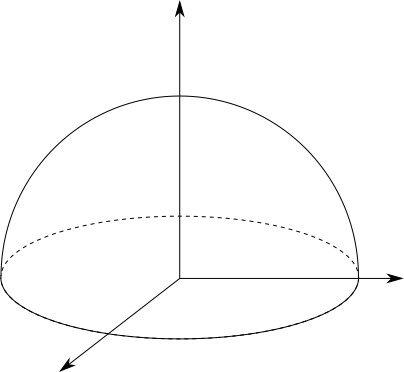
\includegraphics[width=0.5\textwidth]{hemisphere.svg}
%%     \caption{Upper hemisphere}
%%     \label{hemisphere}
%%   \end{figure}
%% }{
  \begin{figure}[H]
    \centering
    \def\svgwidth{0.5\columnwidth}
    \input{figures/latex/hemisphere.pdf_tex}
    \caption{Upper hemisphere}
    \label{hemisphere}
  \end{figure}
%% }
    
    Therefore in spherical coordinates, the limits will be given by
      \[
        0 \leq r \leq 2, \quad 0 \leq \varphi \leq \frac{\pi}{2}, \quad 0 \leq \theta \leq 2\pi.
      \]
    To express the integrand in spherical coordinates, we use
      \[
        x^2 + y^2 + z^2 = r^2 \text{ and } z = r\cos(\varphi).
      \]
    Thus we have
      \[
        z^2\sqrt{x^2 + y^2 + z^2} = r^2\cos^2(\varphi) \times \sqrt{r^2} = r^3\cos^2(\varphi).
      \]
    Hence the integral is
      \begin{align*}
        & \phantom{=} \int\nolimits_0^{2\pi} \int\nolimits_0^{\pi/2} \int\nolimits_0^2 \left(r^3\cos^2(\varphi)\right) \times \left(r^2\sin(\varphi)\right) \, dr \, d\varphi \, d\theta  \\
        & = \int\nolimits_0^{2\pi} \int\nolimits_0^{\pi/2} \int\nolimits_0^2 r^5\cos^2(\varphi)\sin(\varphi) \, dr \, d\varphi \, d\theta  \\
        & = \int\nolimits_0^{2\pi} \int\nolimits_0^{\pi/2} \left[\frac{1}{6}r^6\cos^2(\varphi)\sin(\varphi)\right]_0^2 \, d\varphi \, d\theta  \\
        & = \int\nolimits_0^{2\pi} \int\nolimits_0^{\pi/2} \frac{32}{3}\cos^2(\varphi)\sin(\varphi) \, d\varphi \, d\theta  \\
        & = \frac{32}{3} \int\nolimits_0^{2\pi} \left[-\frac{1}{3}\cos^3(\varphi)\right]_0^{\pi/2} \, d\theta  \\
        & = \frac{32}{9} \int\nolimits_0^{2\pi} \cos^3(0) - \cos^3\left(\frac{\pi}{2}\right) \, d\theta  \\
        & = \frac{32}{9} \int\nolimits_0^{2\pi} 1 \, d\theta  \\
        & = \frac{32}{9}\left[\theta\right]_0^{2\pi}  \\
        & = \frac{64}{9}\pi.
      \end{align*}
  \end{example}
  
  \subsubsection*{Surfaces given by constant values of $r$, $\theta$, $\varphi$}
  
  \begin{itemize}
    \item $r = a$, $a$ constant: sphere of radius $a$, centre at the origin.
    \item $\theta = \alpha$, $\alpha$ constant: half-plane perpendicular to the $(x, y)$-plane, bounded by the $z$-axis; $\alpha$ is the (anticlockwise) angle with the positive $x$-axis.
    \item $\varphi = \beta$, $\beta$ constant: varies depending on $\beta$.
      \begin{itemize}
        \item $\beta = 0$ gives the positive $z$-axis (not a surface).
        \item $0 < \beta < \dfrac{\pi}{2}$ gives a cone, centred around the positive $z$-axis, vertex at the origin; $\beta$ is the angle with the positive $z$-axis.
        \item $\beta = \dfrac{\pi}{2}$ gives the $(x, y)$-plane.
        \item $\dfrac{\pi}{\strut 2} < \beta < \pi$ gives a cone, centred around the negative $z$-axis, vertex at the origin; $\beta$ is the angle with the positive $z$-axis, so $\pi - \beta$ is the angle with the negative $z$-axis.
        \item $\beta = \pi$ gives the negative $z$-axis.
      \end{itemize}
  \end{itemize}
  
  Planes parallel to the $(x, y)$-plane are not given by constant functions in spherical coordinates (other than the $(x, y)$-plane itself).
  
  Consider a point the plane $z = a$, where $a$ is constant.  Then
    \[
      z = a = r\cos(\varphi),
    \]
  so, rearranging,
    \[
      r = \frac{a}{\cos(\varphi)} = a\sec(\varphi).
    \]
  
  For $0 \leq \varphi < \dfrac{\pi}{2}$, this gives the plane $z = a$.
  
  For $\dfrac{\pi}{2} < \varphi \leq \pi$, this gives the plane $z = - a$.
  
  \subsubsection*{Determining limits of regions in spherical coordinates}
  
  See the handout, distributed in the Wednesday Week 10 lecture, and also available on the Week 10 section of the course Moodle page.
  
  Note: this handout comes from a book (\emph{Calculus} by Anton, Bivens, and Davis), and uses $\rho$ in place of $r$ and $\phi$ in place of $\varphi$.
  
  \begin{example}
    Given a 3-dimensional region $G$, the triple integral
      \[
        \iiint_G 1 \, dV
      \]
    gives the volume of $G$.  (Often the $1$ is omitted.)  We will use this to derive the standard formula for the volume of a sphere.
    
    Let $G$ be a sphere of radius $a$, centred at the origin.  Then the volume $V$ of $G$ is
      \begin{align*}
        V = \iiint_G dV & = \int_0^{2\pi} \int_0^{\pi} \int_0^a r^2 \sin(\varphi) \, dr \, d\varphi \, d\theta  \\
        & = \int_0^{2\pi} \int_0^{\pi} \left[\frac{r^3}{3}\right] \sin(\varphi) \, d\varphi \, d\theta  \\
        & = \frac{a^3}{3} \int_0^{2\pi} \int_0^{\pi} \sin(\varphi) \, d\varphi \, d\theta  \\
        & = \frac{a^3}{3} \int_0^{2\pi} \left[- \cos(\varphi)\right]_0^{\pi} \, d\theta  \\
        & = \frac{a^3}{3} \int_0^{2\pi} 2 \, d\theta = \frac{4\pi a^3}{3}.
      \end{align*}
  \end{example}
  
  
    
  
  
% VOLUME is now just an example!
  
%  \subsection{Volume calculated as a triple integral}
%  
%  Consider a triple integral in which the integrand is $1$:
%    \[
%      \iiint_G 1 \, dV.
%    \]
%  This is often written simply as
%    \[
%      \iiint_G dV.
%    \]
%  What does this integral give us?  Consider the case when $G$ is a simple $xy$-solid:
%  
%  \begin{figure}[H]
%    \centering
%    \def\svgwidth{0.65\columnwidth}
%    \input{diagrams/tripleintegral3dregion.pdf_tex}
%  \end{figure}  
%  
%  with:
%    \begin{itemize}
%      \item lower surface $z = g_1(x, y)$;
%      \item upper surface $z = g_2(x, y)$;
%      \item projection $R$ onto the $(x, y)$-plane.
%    \end{itemize}
%  
%  Then
%    \begin{align*}
%      \iiint_G 1 \, dV & = \iint_R \left[\int\nolimits_{g_1(x, y)}^{g_2(x, y)} 1 \, dz\right] \, dA  \\
%      & = \iint_R \left[z\right]_{g_1(x, y)}^{g_2(x, y)} \, dA  \\
%      & = \iint_R g_2(x, y) - g_1(x, y) \, dA  \\
%      & = \underbrace{\iint_R g_2(x, y) \, dA}_{\text{volume under } g_2(x, y)} - \underbrace{\iint_R g_1(x, y) \, dA}_{\text{volume under } g_1(x, y)}.
%    \end{align*}
%    
%  Thus this triple integral gives the volume of the region $G$.
%    
%  In fact, this works for other regions, not just simple $xy$-solids.
%    
%  \subsubsection*{Alternative argument}
%    
%  Consider a solid $G$ with density given by $\delta(x, y, z)$ at a point $(x, y, z)$.  The mass $M$ of the solid is given by
%    \[
%      M = \iiint_G \delta(x, y, z) \, dV.
%    \]
%  (See Worksheet 9, question 3.)
%  
%  Suppose the density of $G$ is a constant $D$, and write $V$ for the volume of $G$.  Then
%    \[
%      D = \frac{M}{V}.
%    \]
%  If $D = 1$, this becomes
%    \[
%      1 = \frac{M}{V} = \frac{\iiint\limits_G 1 \, dV}{V}.
%    \]
%  Rearranging gives
%    \[
%      V = \iiint_G 1 \, dV.
%    \]
%  
%  \begin{examples} \ 
%  
%    \begin{enumerate}
%      \item Find the volume of the solid within the cylinder $x^2 + y^2 = 9$ and between the planes $z = 1$ and $x + z = 5$.
%      
%      Write $G$ for this solid.  It is a simple $xy$-solid, with lower surface $z = 1$ and upper surface $z = 5 - x$.  The projection of $G$ onto the $(x, y)$-plane is the circular region bounded by $x^2 + y^2 = 9$; we denote this region by $R$.  Hence the volume is
%        \begin{align*}
%          V = \iiint_G \, dV & = \iint_R \left[\int\nolimits_1^{5 - x} \, dz\right] \, dA  \\
%          & = \int\nolimits_{-3}^{3} \int\nolimits_{-\sqrt{9 - x^2}}^{\sqrt{9 - x^2}} \int\nolimits_1^{5 - x} \, dz \, dy \, dx  \\
%          & = \int\nolimits_{-3}^{3} \int\nolimits_{-\sqrt{9 - x^2}}^{\sqrt{9 - x^2}} \left[z\right]_1^{5 - x} \, dy \, dx  \\
%          & = \int\nolimits_{-3}^{3} \int\nolimits_{-\sqrt{9 - x^2}}^{\sqrt{9 - x^2}} 4 - x \, dy \, dx  \\
%          & = \int\nolimits_{-3}^{3} \left[(4 - x)y\right]_{-\sqrt{9 - x^2}}^{\sqrt{9 - x^2}} \, dx  \\
%          & = \int\nolimits_{-3}^{3} (8 - 2x)\sqrt{9 - x^2} \, dx  \\
%          & = 8\int\nolimits_{-3}^{3} \sqrt{9 - x^2} \, dx - \int\nolimits_{-3}^{3} 2x\sqrt{9 - x^2} \, dx  \\
%        \end{align*}
%      The first of these integrals with respect to $x$ could be calculated using the techniques for integrating functions involving square roots from Section~\ref{sect:sqrts}.  However, to make things simpler for us, observe that it is the area of the positive half of a circular disc of radius $3$ (centred at the origin).  Thus we have
%        \[
%          \int\nolimits_{-3}^{3} (8 - 2x)\sqrt{9 - x^2} \, dx = \frac{1}{2} \times 3^2 \pi = \frac{9}{2}\pi.
%        \]
%      For the second integral, it is straightforward to use a suitable substitution, but again, we can simplify the calculation by observing that the integrand,
%        \[
%          2x\sqrt{9 - x^2},
%        \]
%      is an odd function, and the interval of integration is $[-3, 3]$.  Thus this integral is $0$.  Hence the volume of the solid is
%        \[
%          V = 8\left(\frac{9}{2}\pi\right) - 0 = 36\pi.
%        \]
%      \item Find the volume of the solid $G$ bounded by the sphere $x^2 + y^2 + z^2 = 16$ and below by the cone $z = \sqrt{x^2 + y^2}$.
%      
%      The region $G$ is an ice-cream-cone-shaped solid cut from a sphere, so in this example we will use spherical coordinates.  In spherical coordinates, the equation of the sphere $x^2 + y^2 + z^2 = 16$ is $r = 4$, and the equation of the cone $z = \sqrt{x^2 + y^2}$ is
%        \begin{align*}
%          r\cos(\varphi) & = \sqrt{r^2\sin^2(\varphi)\cos^2(\theta) + r^2\sin^2(\varphi)\sin^2(\theta)}  \\
%          & = \sqrt{r^2\sin^2(\varphi)\left(\cos^2(\theta) + \sin^2(\theta)\right)}  \\
%          & = \sqrt{r^2\sin^2(\varphi)}  \\
%          & = r\sin(\varphi).
%        \end{align*}
%      Dividing both sides by $r\cos(\varphi)$ gives
%        \[
%          \tan(\varphi) = 1,
%        \]
%      so this cone is given by $\varphi = \dfrac{\pi}{4}$.  Using the \emph{Determination of Limits} handout to determine the limits for the triple integral, the volume of $G$ is given by
%        \begin{align*}
%          V = \iiint_G dV & = \int\nolimits_0^{2\pi} \int\nolimits_0^{\pi/4} \int\nolimits_0^4 r^2\sin(\varphi) \, dr \, d\varphi \, d\theta  \\
%          & = \int\nolimits_0^{2\pi} \int\nolimits_0^{\pi/4} \left[\frac{r^3}{3}\right]_0^4 \, d\varphi \, d\theta  \\
%          & = \int\nolimits_0^{2\pi} \int\nolimits_0^{\pi/4} \frac{64}{3}\sin{\varphi} \, d\varphi \, d\theta  \\
%          & = \frac{64}{3} \int\nolimits_0^{2\pi} \left[-\cos(\varphi)\right]_0^{\pi/4} \, d\theta  \\
%          & = \frac{64}{3} \int\nolimits_0^{2\pi} \left(1 - \frac{\sqrt{2}}{2}\right) \, d\theta  \\
%          & = \frac{64\pi}{3}(2 - \sqrt{2}).
%        \end{align*}
%    \end{enumerate}
%  \end{examples}
  
  
  
  
  
  
  
  


%% \newpage
%% \section{Ordinary Differential Equations (ODEs)}

% AIMS: cut as with other sections.
%\subsection*{Aims}
%\begin{itemize}
%\item Describing basic ideas of ODEs
%\item Solve first order ODEs
%\item Solve linear second order ODEs
%\end{itemize}

Differential equations are widely used in science, engineering and economics.  After 400 years there are still lots of open problems to solve.

\subsection{Overview}

A differential equation is an equation which links $y$,\quad
$\dfrac{dy}{dx}$, \quad $\dfrac{d^2 y}{dx^2}$, etc.

\begin{examples}\quad
\begin{tabular}{ll}
$\dfrac{dy}{dx}  =  x$ & Easy \\
$\dfrac{dy}{dx}  =  x + y^2$ & Hard \\
$\left(\dfrac{dy}{dx}\right)^2 + \left(\dfrac{dy}{dx}\right)  =  \sin(y)$ & Very hard \\
$\dfrac{d^2y}{dx^2} + \dfrac{dy}{dx}  =  \sin(x)$ & Easy
\end{tabular}
\end{examples}

``Ordinary'' means there is only one independent variable.

\subsection*{Some terminology}

\begin{itemize}
\item The \textbf{order} of a differential equation is the largest
number of derivatives.

\begingroup
\renewcommand{\arraystretch}{2}
\begin{tabular}[3]{ll}
$\dfrac{dy}{dx}  =  x$ & \textbf{First} order \\
$\dfrac{d^2y}{dx^2}  =  x$ & \textbf{Second} order \\
$\dfrac{d^4y}{dx^4} + p \dfrac{d^2y}{dx^2} + y  =  0$ &
\textbf{Fourth} order
\end{tabular}
\endgroup

\item A differential equation is \textbf{linear} if we only have
$\dfrac{d^2y}{dx^2}$, $\dfrac{dy}{dx}$ or $y$ and no functions such
as $y^2$.

\begin{itemize}
\item Linear equations are easy to solve and very common.

\item Nonlinear equations are often \textbf{very} hard to
solve.  The solutions usually use numerical methods.
\end{itemize}

\item The \textbf{initial condition(s)} of a differential equation
is information about the solution at a point $x=a$. We need this to find a particular solution to the equation; that is, one that does not depend on any arbitrary constants.

\begin{tabular}{ll}
 First order: & Need to know $y(a)$ \\\\
 Second order: & Need to know $y(a)$, $\dfrac{dy(a)}{dx}$
\end{tabular}
\end{itemize}



\subsection{Separable first order differential equations}  \label{sect:sepdiff}

\begin{definition}
A \textbf{separable} first order ordinary differential equation has
the form
\[
\dfrac{dy}{dx}  =  p(x)q(y).
\]
\end{definition}

We can solve these \textbf{directly by integration}:

Rearrange and integrate
\begin{align*}
\dfrac{1}{q(y)} \dfrac{dy}{dx}  & =  p(x)  \\
\implies \int \dfrac{1}{q(y)} \dfrac{dy}{dx}dx & = \int p(x)dx  \\
\implies \int \dfrac{dy}{q(y)} & =  \int p(x)dx
% \label{sepde_eqn}
\end{align*}

\begin{example}
 \[
  \dfrac{dy}{dx} = \dfrac{xe^{x^2}}{y^2}
 \]

 Separate and integrate
 \begin{eqnarray*}
  && \int y^2 dy = \int x e^{x^2} dx\\
  &\Rightarrow& \dfrac{y^3}{3} = \dfrac{1}{2} e^{x^2} + c\\
  &\Rightarrow& {y^3} = \dfrac{3}{2} e^{x^2} + c 
 \end{eqnarray*}

\end{example}

\begin{example}
In the introduction to the course we saw a basic model for world population.  A more sophisticated model for population $p(t)$ might satisfy the differential equation
\[
\dfrac{dp}{dt}  = p(M-p).
\]

Separating variables and integrating gives
\begin{eqnarray*}
&& \int \dfrac{dp}{p(M-p)}  =  \int dt \\
& &\text{LHS use partial fractions} \\
&& \dfrac{1}{p(M-p)}  =  \dfrac{\dfrac{1}{M}}{p} +
\dfrac{\dfrac{1}{M}}{M-p} \\
&\therefore & \dfrac{1}{M} \ln \left|\dfrac{p}{M-p}\right|
 =  t + C.
\end{eqnarray*}

To find $C$ we need some initial data. Let $p=p_0$ at $t=0$.
\begin{eqnarray*}
&\Rightarrow  & C  =  \dfrac{1}{M} \ln \left|\dfrac{p_0}{M-p_0}\right| \\
&\therefore & \dfrac{1}{M} \ln \left|\dfrac{p}{M-p}\right|
 =  t + \dfrac{1}{M} \ln \left|\dfrac{p_0}{M-p_0}\right|.
\end{eqnarray*}

Multiply by $M$ and exponentiate
\[
\frac{p}{M-p}  =  \dfrac{p_0}{M-p_0} e^{Mt}.
\]

Rearrange
\begin{eqnarray*}
&& p  =  \left[ \dfrac{p_0}{M-p_0} e^{Mt}\right] M - \left[
\dfrac{p_0}{M-p_0} e^{Mt}\right]p \\
&& p\left[1 + \dfrac{p_0}{M-p_0} e^{Mt}\right] = \left( \dfrac{p_0
M}{M-p_0}\right) e^{Mt}
\end{eqnarray*}
\begin{eqnarray*}
\therefore \quad  p  &=&  \dfrac{M p_0 e^{Mt}}{M-p_0+p_0 e^{Mt}}\\
&=&  \dfrac{M p_0 e^{Mt}}{M-p_0} \cdot  \dfrac{M - p_0}{M-p_0+p_0 e^{Mt}}
\end{eqnarray*}
% The last expression doesn't seem helpful.

Sketch:

At $t=0$, 
\[
p = \dfrac{M p_0}{M - p_0 + p_0}=p_0.
\]

As $t \to \infty$,
\[
 \dfrac{Mp_0}{p_0} = M.
\]

%% \nextalt{Request description from lecturer or tactile diagram.}
\begin{figure}[H]
\centering
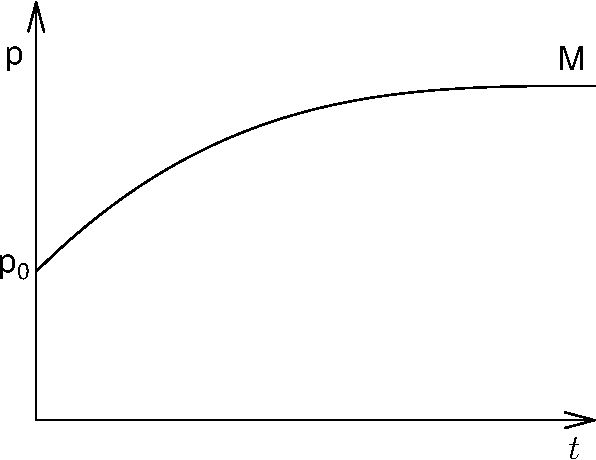
\includegraphics[width=0.5\textwidth]{population-de.pdf}
\caption{Sketch of example}
\label{populationde}
\end{figure}

\end{example}



\subsection{Homogeneous equations}

A function $f(x,y)$ is homogeneous of degree $n$ if
\[
 f(tx,ty) = t^{n} f(x,y).
\]

\begin{examples}
 \quad
 \begin{eqnarray*}
   f(x,y) &=& x^2 + xy\\
  \Rightarrow\quad f(tx, ty) &=& t^2 x^2 + t^2 xy \\
  &=& t^2 f(x,y)
 \end{eqnarray*}
(homogeneous, degree $2$)

 \begin{eqnarray*}
   f(x,y) &=& \sqrt{x^2 + y^2}\\
  \Rightarrow\quad f(tx, ty) &=& t \sqrt{x^2 + y^2} \\
  &=& t f(x,y)
 \end{eqnarray*}
(homogeneous, degree $1$)

\[
 f(x,y) = \sin \left(\dfrac{y}{x}\right)
\]
(homogeneous, degree $0$)
\end{examples}


% There's no higher degree version, but it looks like it is possible to use a similar method using t = 1/x.
\subsubsection*{Degree $0$.}

The general form for a homogeneous differential equation of degree $0$ is
\[
 \dfrac{dy}{dx} = f \left(\dfrac{y}{x}\right)
\]

\begin{solution}
 Let $u=\dfrac{y}{x}$. Then
 \begin{eqnarray*}
  && ux = y\\
  &\Rightarrow& u+x \dfrac{du}{dx} = \dfrac{dy}{dx}.
 \end{eqnarray*}

 Hence
  \begin{eqnarray*}
  && u + x \dfrac{du}{dx} = f(u)\\
  &\Rightarrow& x \dfrac{du}{dx} = f(u) - u\\
  &\Rightarrow& \int \dfrac{du}{f(u)-u} = \int \dfrac{dx}{x} = \ln \left|x\right|+c.
 \end{eqnarray*}
\end{solution}

\begin{example}
 \[
  \dfrac{dy}{dx} = \dfrac{y}{x} \left(1 + \ln \left(\dfrac{y}{x}\right)\right)
 \]
 
 Let $u=\dfrac{y}{x}$. Then
 \begin{eqnarray*}
  u + x \dfrac{du}{dx} &=& u (1 + \ln(u))\\
  &=& u + u \ln (u)\\
  \Rightarrow \quad \int \dfrac{du}{u \ln(u)} &=& \int \dfrac{dx}{x} \\
  &=& \ln \left|x\right| + c.
 \end{eqnarray*}

 Let $v=\ln(u)$. Then
 \[
  \dfrac{dv}{du} = \dfrac{1}{u} \qquad (u>0)
 \]

 So
 \[
  \int \dfrac{du}{u \ln(u)} = \int \dfrac{dv}{v} = \ln \left|v\right|
 \]
 
 Hence
 \[
  \ln \left|v\right| = \ln (x)+c
 \]
 
 If $v>0$, \quad $v=Ax$, \quad $A=e^{c}$.

\begin{eqnarray*}
& \Rightarrow & \ln (u) = Ax\\
& \Rightarrow & \ln \left(\dfrac{y}{x}\right) = Ax\\
& \Rightarrow & u=xe^{Ax}.
\end{eqnarray*}
\end{example}


\subsection{Linear first order ordinary differential equations}

These take the form
\begin{equation*}
\dfrac{dy}{dx} + p(x)y  =  q(x).
\label{lin_ODE}
\end{equation*}
The LHS is a linear combination of $y$ and its derivative.


We solve these by using an \textbf{integrating factor}. 


\begin{lemma}
If $r(x) = e^{\int p(x)dx}$ then
\[
\dfrac{dr}{dx}  =  p(x) r(x).
\]
\end{lemma}

\begin{Proof}
By chain rule
\begin{eqnarray*}
 \dfrac{dr}{dx}  &=&  e^{\int p(x)dx} \dfrac{d}{dx} \int
p(x)dx\\
&=& p(x) e^{\int p(x)dx} \\
&& \text{by Fundamental theorem of calculus}\\
&=& p(x) r(x)
\end{eqnarray*}
\end{Proof}

The function $r(x) =  e^{\int p(x)dx}$ is called the \emph{integrating factor}.

\begin{proposition}
The equation
\begin{equation}
 \dfrac{dy}{dx} + p(x)y = q(x)
 \label{eq5.1}
\end{equation}
has solution
\[
 y(x) = \dfrac{1}{r(x)} \int r(x)q(x)dx.
\]
\end{proposition}

\begin{Proof}
Consider
\begin{eqnarray*}
 && \dfrac{d}{dx} (r(x)y(x)) \\
 &=& r(x) \dfrac{dy}{dx} + y \dfrac{dr}{dx}\\
 &=& r(x) \dfrac{dy}{dx} + y pr\\
 &=& r(x) \left(\dfrac{dy}{dx} + y p\right)
\end{eqnarray*}

Hence if $y$ satisfies \eqref{eq5.1}, then
\begin{eqnarray*}
 && \dfrac{d}{dx}(ry) = r \left(\dfrac{dy}{dx}+py\right) = rq\\
 &\Rightarrow& y = \dfrac{1}{r} \int rq dx.
\end{eqnarray*}
\end{Proof}


\begin{examples}
\quad

\begin{enumerate}
 \item $\dfrac{dy}{dx} + y  =  x$

 So
 \[
  \dfrac{dy}{dx} + p(x)y = q(x),
 \]
where
\[
p(x) = 1, \quad q(x) = x.
\]

Integrating factor:
\begin{eqnarray*}
r(x) = e^{\int p(x)dx}
 =  e^x.
 \end{eqnarray*}
 
Hence
\begin{eqnarray*}
y(x) &=&  e^{-x} \int e^x x dx\\
&=&  e^{-x} [xe^{x} - e^{x} + c]\\
&=&  x - 1 + ce^{-x}.
\end{eqnarray*}
(note: non-trivial constant)

\item $x \dfrac{dy}{dx} + 2 u  =  x^3$

Rearranging,
\[
 \frac{dy}{dx} + 2 \frac{y}{x}  =  x^2 ,
\]
so
\[
 \frac{dy}{dx} + p(x)y  =  q{x}, 
\]
where $p(x)=\dfrac{2}{x}$, $q(x) = x^2$.

Integrating factor:
\begin{eqnarray*}
 r(x) &=& e^{\int \frac{2}{x}dx} \\
 &=& e^{2\ln(x)}\\
 &=& x^2.
\end{eqnarray*}

Hence
\begin{eqnarray*}
 y(x) &=& \dfrac{1}{x^2} \int x^2 x^2 dx \\
 &=& \dfrac{1}{x^2} \left[\dfrac{x^5}{5}+c\right]\\
 &=& \dfrac{x^3}{5} + \dfrac{c}{x^2}.
\end{eqnarray*}

% I have never done this long and tedious example in the lecture.
% Omitting it from the lecture notes for now.

%% Definitely a problems class example.
%% Also from "Now, for constants..." I think it could use some work to make it more easy to follow.
%\item Climate: Why is February such a rotten month (in England)?
%
%\nextalt{Request description from lecturer or tactile diagram.}
%\begin{figure}[H]
%\centering
%\includegraphics[width=0.55\textwidth]{climate.pdf}
%\caption{Climate}
%\label{climate}
%\end{figure}
%
%$t$:\quad years;  $t=0$  on 21st Dec. (Winter Solstice)
%% Winter Solstice is actually 22nd December this year.
%
%$S$:\quad sunshine, modelled as
%\[
%S(t)=\overline{s} (1-\cos(2\pi t)).
%\]
%
%$T$:\quad Kelvin; the sea (surface) temperature.
%
%Newton's law of cooling:
%\[
 %\frac{dT}{dt}  =  -k (T - S(t)) 
%\]
%($k$ constant)
%
%Rearranging
%\[
 %\frac{dT}{dt} + k T  =  k S(t)
%\]
%
%So this is in the form \eqref{eq5.1}
%with $p(t)=k$, $q(t)=k S(t)$.
%
 %Integrating factor:
 %\[
  %r(t) = e^{\int kdt} = e^{kt}.
 %\]
%
 %Hence
 %\begin{eqnarray*}
  %T(t) &=& e^{-kt} \int e^{kt} k S(t) dt\\
   %&=& \overline{s} k e^{-kt} \int e^{kt} (1-\cos(2\pi t)) dt
 %\end{eqnarray*}
%
%Now, for constants $a,b\in\RR$ we have
%\begin{eqnarray*}
 %&& \int e^{at} \cos(bt) dt 
%=%\\ &=&
 %\dfrac{e^{at}}{a^2+b^2}  [a \cos(bt) + b \sin (bt)] + c.
%\end{eqnarray*}
%
%Hence the sea surface temperature is 
%\begin{eqnarray*}
%T(t) &=& \overline{s} ke^{-k t} \left(\frac{e^{k t}}{k} 
%- \frac{ e^{k t}}{k^2+4\pi^2} \left[k \cos(2\pi t) + 2\pi
%\sin(2\pi t)\right] + c\right)
%\\
%&=& \underbrace{\overline{s}}
%- \underbrace{\dfrac{\overline{s}k}{k^2+4\pi^2}
%\left[k \cos(2\pi t) + 2\pi\sin(2\pi t)\right]}
%+ \underbrace{c \overline{s} k e^{-k t}.}
%\\&&\text{base\hspace{2.5cm}seasonality\hspace{2cm}transient effect}
%\end{eqnarray*}
%
%Aside:
%\let\thhh=\theta\def\theta{\chi}%%% fix theta to chi temporarily
%
%Consider $$a \cos(x) + b \sin(x).$$
%%
%For $\theta$ such that $\tan (\theta)=\dfrac{b}{a}$ we have
%\[
 %\sin (\theta) = \dfrac{b}{\sqrt{a^2+b^2}}, \qquad \cos(\theta) = \dfrac{a}{\sqrt{a^2+b^2}}
%\]
%Then
%\begin{eqnarray*}
%&& \sqrt{a^2+b^2} \cos (x-\theta)\\
%&&= \sqrt{a^2+b^2} [\cos(x) \cos{\theta} + \sin(x) \sin(\theta)]\\
%&&= a \cos(x) + b \sin(x)
%\end{eqnarray*}
%Hence%, take $a=k,\ b=2\pi,\ x=2\pi t$,
%\begin{eqnarray*}
 %&& k \cos(2\pi t) + 2 \pi \sin(2\pi t)
 %\\ &&= 
%\sqrt{k^2+4\pi^2} \cos(2\pi t-\theta)
%\end{eqnarray*}
%where \[\tan(\theta)=\dfrac{2\pi}{k}\]
%and $\theta$ is the phase shift or lag wrt.\ the sunshine intensity $S(t)$.
%
%Thus, after transient worn off
%\[
 %T(t) \simeq \overline{s} \left(
 %1 - \dfrac{k}{\sqrt{k^2+4\pi^2}} \cos \left(2\pi\left(t-\dfrac{\theta}{2\pi}\right)\right)
 %\right)
%\]
%\\
%On our %island
%sea coast 
%$k\approx8$ is 'large', 
%%$k\approx7$, 
%%
%so $$\dfrac{\theta}{2\pi}=\dfrac{1}{2\pi}\arctan\left(\dfrac{2\pi}{k}\right)
%\approx\dfrac1k
%\approx\dfrac18\text{  (years) $\cong$ 1.5 (months),}$$
 %so the sea is coldest in February (= 21st Dec.+1.5 months).
%%\approx\dfrac19\text{  (years) $\cong$ 6 (weeks),}$$
%% so the sea is coldest in February (= 21st Dec.+6 weeks).
%
%\nextalt{Request description from lecturer or tactile diagram.}
%\iftoggle{clearprint}{
%\begin{figure}[H]
%\centering
%\boldmath
%\includegraphics[width=0.6\textwidth]{periodic_response.pdf} \\
%\raisebox{1.1cm}[0pt][0pt]{\hspace{.1cm}$/2\pi$\hspace{2.3cm}$/2\pi$}\\[-.5cm]
%\caption{Steady periodic response. Legend: $S$ -- red; $T$ -- blue.}
%\label{periodicresponse}
%\end{figure}
%}{
%\iftoggle{web}{
%\begin{figure}[H]
%\centering
%\includegraphics[width=0.6\textwidth]{periodic_response-byhand.svg}
%\caption{Steady periodic response. Legend: $S$ -- red; $T$ -- blue.}
%\label{periodicresponse}
%\end{figure}
%}{
%\begin{figure}[H]
%\centering
%\boldmath
%\includegraphics[width=0.6\textwidth]{periodic_response.pdf} \\
%\raisebox{.9cm}[0pt][0pt]{\hspace{.1cm}$/2\pi$\hspace{2.3cm}$/2\pi$}\\[-.5cm]
%\caption{Steady periodic response. Legend: $S$ -- red; $T$ -- blue.}
%\label{periodicresponse}
%\end{figure}
%}}
%\let\theta=\thhh

\end{enumerate}
\end{examples}

\subsection{Bernoulli equations}

A differential equation of the form
\[
 \dfrac{dy}{dx} + p(x)y = q(x)y^{n}, \quad n \in \ZZ
\]
is called a Bernoulli equation (named after Jacob Bernoulli, who proposed it, and his brother Johann Bernoulli, who found a solution).

If $n=0$ or $1$ they are linear. Solve by integrating factor ($n=0$) or separation ($n=1$). 
Otherwise they are non-linear.

\emph{Method} for $n\ne0$ or $1$.

Idea: use a substitution to make the equation linear.

Divide by $y^{n}$:
\[
 y^{-n} \dfrac{dy}{dx} + p(x) y^{1-n} = q(x)
\]

Let $z=y^{1-n}$.  Then by the chain rule
\[
 \dfrac{dz}{dx} = (1-n) y^{-n} \dfrac{dy}{dx} .
\]

Substitute 
\[
 \dfrac{1}{1-n} \dfrac{dz}{dx} + p(x) z= q(x)
\]

This equation is now \emph{linear} in the  $z$-terms: use integrating factor to solve.

%\newpage

\begin{examples}\
\begin{enumerate}
 
 \item $\dfrac{dy}{dx} + \dfrac{4}{x}y = x^3 y^2$
 
 Bernoulli equation with
 \[
  p(x)=\dfrac{4}{x}, \quad q(x)=x^3, \quad n=2.
 \]

 Divide by $y^2$
 \[
  y^{-2} \dfrac{dy}{dx} + \dfrac{4}{x} y^{-1} = x^3
 \]
 
 Let $z=y^{-1}$. So
$
  \dfrac{dz}{dx} = -y^{-2} \dfrac{dy}{dx}.
$

 Substitute
 \begin{eqnarray*}
  && -\dfrac{dz}{dx} + \dfrac{4}{x} z = x^{3}\\
  &\Rightarrow& \dfrac{dz}{dx} - \dfrac{4}{x} z = -x^{3}
 \end{eqnarray*}

 Integrating factor
 \[
  r(x) = e^{\int -\frac{4}{x}dx} = e^{\int -4\ln\left|x\right|} = x^{-4}.
 \]

 Then
 \begin{eqnarray*}
  z(x) &=& \dfrac{1}{r(x)} \int r(x) q(x) dx\\
  &=& x^4 \int x^{-4}(-x^3)dx\\
  &=& x^4 \int -x^{-1}dx\\
  &=& x^4 (-\ln\left|x\right|+c)\\
  &=& x^4 (c-\ln\left|x\right|).
 \end{eqnarray*}

 Hence
 \[
  y=\dfrac{1}{x^4(c-\ln\left|x\right|)}.
 \]



 \item $\dfrac{dy}{dx} = 5y + e^{-2x}y^{-2}$
 
 Rearrange 
 \[
  \dfrac{dy}{dx} - 5y = e^{-2x} y^{-2}
 \]

 Bernoulli equation with $$p(x)=-5,\ q(x)=e^{-2x},\ n=-2.$$

So $z=y^{1-n}=y^{3}$ satisfies
\begin{eqnarray*}
&& \dfrac{1}{1-n} \dfrac{dz}{dx} + p(x) z= q(x)\\
\iff&&
  \dfrac{1}{3} \dfrac{dz}{dx} - 5z = e^{-2x}.
\end{eqnarray*}

Rearrange 
\[
 \dfrac{dz}{dx} - 15z = 3e^{-2x}
\]


 Integrating factor
 \[
  r(x) = e^{\int -15dx} = e^{-15x}
 \]

 So
 \begin{eqnarray*}
  z(x) &=& e^{15x} \int e^{-15x} (3e^{-2x})dx\\
  &=& e^{15x} \left[ -\dfrac{3}{17} e^{-17x} + c \right]
%\\  &=& ce^{15x} -\dfrac{3}{17} e^{-2x} 
 \end{eqnarray*}

 Then \[
y=z^{\frac{1}{3}}=e^{5x}\sqrt[3]{c-\dfrac{3}{17} e^{-17x} }
\]

%\newpage

\item
 $6\dfrac{dy}{dx} - 2y = xy^{4}$
 
 Rearrange
 \[
  \dfrac{dy}{dx} - \dfrac{y}{3} = \dfrac{x}{6}y^{4}
 \]

 Bernoulli equation with $$p(x)=-\dfrac{1}{3},\ q(x)=\dfrac{x}{6},\ n=4.$$
 
So $z=y^{1-n}=y^{-3}$ satisfies
\begin{eqnarray*}
&& \dfrac{1}{1-n} \dfrac{dz}{dx} + p(x) z= q(x)\\
\iff&&
  -\dfrac{1}{3} \dfrac{dz}{dx} - \dfrac{z}{3} = \dfrac{x}{6}.
\end{eqnarray*}


Rearrange
 \[
  \dfrac{dz}{dx} + z = -\dfrac{x}{2}
 \]

Integrating factor
\[
 r(x) = e^{\int 1 dx} = e^{x}
\]

Hence
\begin{eqnarray*}
 z(x) &=& e^{-x} \int e^{x} \left(-\dfrac{x}{2}\right) dx\\
 &=& e^{-x}  \left[-\dfrac{1}{2}(xe^{x}-e^{x}) + c\right]\\
 &=& ce^{-x} - \dfrac{1}{2} (x-1)
\end{eqnarray*}

Then $y=z^{-\frac{1}{3}}$.

\item Logistic growth: (e.g. population)\qquad
 $\dfrac{dy}{dx} =y(M-y)$
\qquad (see Section~\ref{sect:sepdiff})
 
 Rearrange
 \[
  \dfrac{dy}{dx} - My = -y^2
 \]
to Bernoulli equation with $$p(x)=-M,\ q(x)=-1,\ n=2.$$
 
So $z=y^{1-n}=y^{-1}$ satisfies
%\begin{eqnarray*}
%&& \dfrac{1}{1-n} \dfrac{dz}{dx} + p(x) z= q(x)\\
%\iff&&
%  - \dfrac{dz}{dx} - Mz = -1.
%\end{eqnarray*}
%
%
%Rearrange
 \[
  \dfrac{dz}{dx} + Mz = 1
 \]

Integrating factor
$
 r(x) = e^{\int M dx} = e^{Mx}
$
gives
\begin{eqnarray*}
 z(x) &=& e^{-Mx} \int e^{Mx}  dx\\
 &=& e^{-Mx}  \left[\dfrac{e^{Mx}}M+ c\right]
=%\\ &=& 
\dfrac1M+ce^{-Mx}
\\
\Rightarrow
\quad y&=&z^{-1}=\left[\dfrac1M+ce^{-Mx}\right]^{-1}=\dfrac M{1+\tilde ce^{-Mx}}
%\qquad\text{(cf. Section 5.1)}
.
\end{eqnarray*}

\end{enumerate}

\end{examples}

% NOTE: Leave this section unchanged for now.  It includes some partial derivatives that have not been covered yet, and the chain rule in two variables.  THIS IS BAD.
% ALSO this may end up being the problems class/extra lecture material.  (It's starred on the problem sheet.)

\subsection{Exact equations}  \label{sect:exact}

Consider a differential equation of the form 
\[
 M(x,y) + N(x,y) \dfrac{dy}{dx} = 0.
\]

This includes functions of two variables $x$ and $y$.

Suppose there exists some function $f(x,y)$ such that
\[
 \dfrac{\partial f}{\partial x} = M
\]
(``partial derivative'': rate of change with respect to $x$ if $y$ held constant)
\[
 \dfrac{\partial f}{\partial y} = N
\]
(rate of change with respect to $y$ if $x$ held constant)

Then
\begin{eqnarray*}
 \dfrac{\partial f}{\partial x} + \dfrac{\partial f}{\partial y} \dfrac{dy}{dx} &=& M + N \dfrac{dy}{dx}\\
 &=& 0
\end{eqnarray*}

Now, the chain rule for two variables says:
\[
 \dfrac{df}{dx} = \dfrac{\partial f}{\partial x} + \dfrac{\partial f}{\partial y} \dfrac{dy}{dx}
\]

So
\begin{eqnarray*}
 && \dfrac{\partial f}{\partial x} + \dfrac{\partial f}{\partial y} \dfrac{dy}{dx} = 0 \\
 &\Rightarrow& \dfrac{df}{dx} = 0\\
 &\Rightarrow& f(x,y) = c.
\end{eqnarray*}

So $f(x,y)=c$ is an \emph{implicit} solution to the differential equation, i.e. if $x,y$ satisfy $f(x,y)=c$, they will also satisfy the ODE.

\subsection*{Test for exactness}

The equation
\[
 M(x,y) + N(x,y) \dfrac{dy}{dx} = 0
\]
is exact if $\dfrac{\partial M}{\partial y}=\dfrac{\partial N}{\partial x}$.

\subsection*{Finding the solution $f(x,y)$}

We can find $f$ by integrating $M$ or $N$, but we have to be careful.  We have
  \[
    \frac{\partial f}{\partial x} = M.
  \]
Integrate both sides with respect to $x$:
  \[
    f(x, y) = \int M \, dx + g(y),
  \]
where $g(y)$ is constant with respect to $x$, but may depend on $y$.

What is $g$?  Differentiate both sides with respect to $y$:
  \[
    \frac{\partial f}{\partial y} = \frac{\partial}{\partial y}\int M \, dx + g'(y).
  \]

Rearranging,
  \begin{align*}
    g'(y) & = \frac{\partial f}{\partial y} - \frac{\partial}{\partial y}\int M \, dx  \\
     & = N - \frac{\partial}{\partial y}\int M \, dx.
  \end{align*}

Hence
  \[
    g(y) = \int g'(y) \, dy = \int \left[ N - \dfrac{\partial}{\partial y} \int M \, dx \right] dy
  \]

So an exact ODE has implicit solution $f(x,y)=c$ where
\[
 f(x,y) = \int Mdx + \int \left[
 N - \dfrac{\partial}{\partial y} \int M \, dx
 \right] dy
\]

\begin{examples}\quad
 \begin{enumerate}
  \item $y+x \dfrac{dy}{dx} = 0$
  
  Inspiration:
  \begin{eqnarray*}
   && \dfrac{\partial}{\partial y} (xy) = x\\
   && \dfrac{\partial}{\partial x} (xy) = y
  \end{eqnarray*}
  
  So $f(x,y)=xy$ satisfied 
  \[
  \dfrac{\partial f}{\partial x}=M, \qquad \dfrac{\partial f}{\partial y}=N
  \]
where $M=y$, $N=x$.
  
  Hence solution is $xy=c$.
  
  \item $e^{y} + (xe^{y} + 2y) \dfrac{dy}{dx}=0$.
  
  So
  \begin{eqnarray*}
&&   M=e^{y}, \qquad N=xe^{y} + 2y\\
&\Rightarrow& \dfrac{\partial M}{\partial y} = e^{y}, \qquad \dfrac{\partial N}{\partial x}=e^{y}.
  \end{eqnarray*}

  Hence the ODE is exact. So solution is $f(x,y)=c$ where
  \begin{eqnarray*}
   f(x,y) &=& \int M dx + \int \left(N - \dfrac{\partial}{\partial y} \int Mdx\right)dy\\
   &=& \int e^{y}dx + \int \left(xe^{y} + 2y - \dfrac{\partial}{\partial y} \int e^{y} dx\right) dy\\
   &=& x e^{y} + \int xe^{y} + 2y - xe^{y} dy\\
   &=& xe^{y} + \int 2y dy\\
   &=& xe^{y} + y^{2}
  \end{eqnarray*}

  Hence implicit solution of ODE is
  \[
   xe^{y} + y^{2} = c.
  \]

  
  \item $2xy - 9x^2 + (2y+x^2+1)\dfrac{dy}{dx} = 0$
  
  So
  \begin{eqnarray*}
&&   M=2xy-9x^2, \qquad N=2y+x^2+1\\
&&   \dfrac{\partial M}{\partial y} = 2x, \qquad \dfrac{\partial N}{\partial x}=2x
  \end{eqnarray*}

  Hence exact.

  Next, find $f(x,y)$:
  \begin{eqnarray*}
   \int M dx &=& \int 2xy - 9x^2 dx\\
   &=& x^2 y - 3 x^3
  \end{eqnarray*}

  So
  \begin{eqnarray*}
   f(x,y) &=& x^2y - 3x^3 + \int 2y + x^2 + 1 - \dfrac{\partial}{\partial y} (x^2y-3x^3)dy\\
   &=& x^2y - 3x^3 + \int 2y + x^2 + 1 - x^2 dy\\
   &=& x^2y - 3x^3 + \int 2y + 1 dy\\
   &=& x^2y - 3x^3 + y^2 + y\\
   &=& y^2 + (x^2+1)y - 3x^3
  \end{eqnarray*}

  Hence the ODE has implicit solution 
  \[
   y^2 + (x^2+1) y - 3x^3 = c.
  \]

  \item $2xy^2 + 4 - 2(3-x^2y) \dfrac{dy}{dx} = 0$
  
    So
  \begin{eqnarray*}
&&   M=2xy^2+4, \qquad N=-2(3-x^2y)\\
&&   \dfrac{\partial M}{\partial y} = 4xy, \qquad \dfrac{\partial N}{\partial x}=4xy
  \end{eqnarray*}

  Hence exact.

  Next, find $f(x,y)$.
  \begin{eqnarray*}
   \int M dx &=& \int 2xy^2 + 4 dx\\
   &=& x^2 y^2 + 4x
  \end{eqnarray*}

  Hence
  \begin{eqnarray*}
   f(x,y) &=& x^2 y^2 + 4x + \int -2(3x-x^2y) - \dfrac{\partial}{\partial y} (x^2y^2+4x)dy\\
   &=& x^2y^2 + 4x + \int -2(3-x^2y) -2x^2ydy\\
   &=& x^2y^2 + 4x -\int 6dy\\
   &=& x^2y^2 + 4x - 6y.
  \end{eqnarray*}

  Hence the ODE has implicit solution
  \[
   x^2y^2 + 4x - 6y = c.
  \]

 \end{enumerate}
\end{examples}

% END OF BAD SECTION.


%\newpage 

\subsection{Linear second order ordinary differential equations}

\subsubsection*{Overview}

These take the form
\begin{align*}
a \dfrac{d^2 u}{dx^2} + b \dfrac{du}{dx} + cu & =  0 \qquad
\text{(Free/Unforced)} \\
a \dfrac{d^2 u}{dx^2} + b \dfrac{du}{dx} + cu & =  f(x) \qquad
\text{(Forced)}
\end{align*}

\begin{example}[Falling ball]
\[
m\frac{d^2 y}{dt^2} + k\frac{dy}{dt}  =  -gm.
\]
\end{example}

Each of these equations has an uncountable number of solutions. To
find a \textbf{unique} solution we must specify \textbf{two}
properties of the solution.

\begin{description}
\item[A.] Initial value problem: $u(0) = \alpha$, \quad $u'(0)=\beta$;
$u$ \emph{and} $u'$ at \emph{some} point, 
\\e.g. throwing a ball.

\item[B.] (Dirichlet) Boundary value problem: $u(0) = \alpha$, \quad $u(1)=\beta$;
\\ e.g. making the ball land on target.

\item[C.] (Neumann) Boundary value problem: $u'(0) = \alpha$, \quad
$u'(1)=\beta$;
\\i.e.\ $u'$ at two points, arises in studying biological problems. 

\end{description}


\subsubsection*{Free linear second order ODEs}

\begin{theorem}[Superposition] \label{thm:superposition}
 Let $p(x)$ and $q(x)$ be solutions to the second order ODE
 \[
  a \dfrac{d^2 u}{dx^2} + b \dfrac{du}{dx} + cu  =  0.
 \]
Then
\[
r(x)  =  A p(x) + B q(x)
\]
is also a solution for any constants $A,B$.
\end{theorem}

\begin{Proof}
 Due to the linearity of the derivative
 \begin{align*}
  r & = Ap + Bq  \\
  \Rightarrow r' & = Ap' + Bq'  \\
  \Rightarrow r'' & = Ap'' + Bq''.
 \end{align*}
 Hence
 \begin{eqnarray*}
  && ar'' + br' + cr\\
  &=& A [ap'' + bp' + cp] + B [aq'' + bq' + q]\\
  &=& 0+0 \\
  && \text{(since $p.q$ solutions)}\\
  &=& 0,
 \end{eqnarray*}
  so $r$ is also a solution to the equation.
\end{Proof}

\begin{definition}
We call
 $r=r(x)$  a \emph{linear combination} of $p$ and $q$.
\end{definition}
 \begin{definition}
 $p$ and $q$ are \emph{linearly independent} if there are \emph{no} non-zero constants $A$ and $B$ such that
 \[
  Ap(x) + Bq(x) = 0 \qquad \forall x
 \]
\end{definition}

\begin{note}
 $Ap+Bq=0$ may still  be satisfied at \emph{some} values of $x$.
\end{note}

\begin{theorem}
 A free linear second order ODE has \emph{exactly two} linearly independent solutions.
 Any solution of the ODE are linear combinations of these two solutions.
\end{theorem}
% NO PROOF.
% There isn't one in the books either.

\begin{definition}
Let the free linear second order ODE have two  linearly independent solutions $p(x)$, $q(x)$. 
Then the \emph{general solution} is
\[
 Ap(x) + Bq(x), \qquad \text{$A,B\in\RR$ constants.}
\]
\end{definition}

\begin{example}  Simple harmonic motion (e.g. oscillation of a spring, simple pendulum, molecular vibration)
 \[
  \dfrac{d^2u}{dx^2} + u = 0
 \]

Two linearly independent solutions are $\sin(x)$ and $\cos(x)$.% (check by substitution)

So, general solution is
\[
 u = A \cos(x) + B \sin(x).
\]
\end{example}

%\newpage

\subsubsection*{Constructing the General solution}

Consider
\begin{equation}
 a \dfrac{d^2u}{dx^2} + b \dfrac{du}{dx} + cu = 0
 \label{eq5.2}
\end{equation}

Suppose $u=e^{\lambda x}$, $\lambda$ constant. Then
\[
 a \dfrac{d^2u}{dx^2} + b \dfrac{du}{dx} + cu = (a\lambda^2 + b\lambda +c) e^{\lambda x}
\]

Hence \eqref{eq5.2} is satisfied if $\lambda$ is such that
\[
 a\lambda^2 + b\lambda +c = 0
\]

This quadratic in $\lambda$ is the \emph{auxiliary equation (AE)}.

Solutions are
\[
 \lambda_{1,2} = \dfrac{-b \pm \sqrt{b^2-4ac}}{2a}
\]

Depending on the type of solutions of the AE
there are three cases to distinguish:

\begin{description}
 \item[Case 1.]  ($b^2-4ac>0$)\quad $\lambda_1, \lambda_2$ real and distinct
 
 General solution
 \[
  u = A e^{\lambda_1x} + B e^{\lambda_2 x}
 \]
 
 Solution behaviour: No oscillations;\\
 long term growth ($\lambda_1>0$ or $\lambda_2>0$) or decline ($\lambda_1<0$ and $\lambda_2<0$).
 \begin{note}\

  $e^{\lambda_1x}$ and $e^{\lambda_2x}$ are linearly independent because 
  \[
   \dfrac{e^{\lambda_1x}}{e^{\lambda_2x}} = e^{(\lambda_1-\lambda_2)x}
  \]
is not constant.
 \end{note}


 \item[Case 2.] ($b^2-4ac<0$)\quad $\lambda_1, \lambda_2$ complex conjugates, $\lambda_{1,2} = \alpha \pm i\beta$
 
 General solution
 \[
  u = e^{\alpha x} (A \cos (\beta x) + B \sin (\beta x)).
 \]

Solution behaviour: Oscillatory with long term growth $(\alpha > 0)$ or decline $(\alpha < 0)$.

\begin{proof}

Real and imaginary parts of the roots of the auxiliary equation
\[
\lambda_{1,2} = \alpha \pm i\beta
\]
are $$\alpha = -\dfrac{b}{2a},\qquad\beta=\dfrac{\sqrt{4ac-b^2}}{2a}.$$

Thus
\[
 u_{1,2} = e^{(\alpha \pm i\beta)x}
%, \qquad u_2 = e^{(\alpha - i\beta)}
\]
are solutions of \eqref{eq5.2}.

But $u_1$ and $u_2$ involve complex numbers for all $x$. The ODE is real-valued. We want real-valued solutions.

By Euler's formula
%\[
% e^{\pm i\beta x} = \cos(\beta x) \pm i \sin(\beta x)
%\]
%
%Hence
\begin{eqnarray*}
 u_{1,2}  = e^{\alpha x} [\cos(\beta x) \pm i \sin(\beta x)]
% && u_1 = e^{\alpha x} [\cos(\beta x) + i \sin(\beta x)]\\
% && u_2 = e^{\alpha x} [\cos(\beta x) - i \sin(\beta x)]
\end{eqnarray*}

Recall superposition (Theorem~\ref{thm:superposition}): Linear combinations of $u_1$ and $u_2$ are also solutions (even with complex coefficients).

So
\[
 \dfrac{1}{2}u_1 + \dfrac{1}{2}u_2 = e^{\alpha x} \cos(\beta x)
\]
is a solution, as well as 
\[
 \dfrac{1}{2i}u_1 - \dfrac{1}{2i}u_2 = e^{\alpha x} \sin(\beta x)
\]
is a solution.

Clearly $e^{\alpha x} \cos(\beta x)$, $e^{\alpha x} \sin(\beta x)$ are real-valued and  linearly independent. 

So the general solution is
\[
 A e^{\alpha x} \cos(\beta x) + B e^{\alpha x} \sin(\beta x).
\]
\end{proof}

 \item[Case 3.] ($b^2=4ac$)\quad $\lambda_1=\lambda_2$, so write $\lambda$ for the unique root of the AE.
 
Then $\lambda = - \dfrac{b}{2a}$  is real-valued and the general solution is
 \[
  u=Ae^{\lambda x} + Bx e^{\lambda x}.
 \]

 Solution behaviour: no oscillations, long term growth ($\lambda>0$) or decline ($\lambda<0$).


 \begin{proof}
  If
  \[
   u = Ae^{\lambda x} + B x e^{\lambda x}
  \]
  
  Then
  \begin{eqnarray*}
   &&    u' = \lambda Ae^{\lambda x}+ B e^{\lambda x} + \lambda B x e^{\lambda x}
\\
   &&    u'' = \lambda^2 Ae^{\lambda x}+ 2\lambda B e^{\lambda x} %+ \lambda^2 B e^{\lambda x} 
+ \lambda^2 B x e^{\lambda x}
  \end{eqnarray*}
  
  Hence
  \begin{eqnarray}
   && au'' + bu' +cu \notag\\
   &=& \quad A [a\lambda^2 + b\lambda_1 + c]e^{\lambda x}\label{eq5.3a}\\
   &&  + B [2a\lambda + b]e^{\lambda x}\label{eq5.3b}\\
   &&  + B x [a\lambda^2 + b\lambda + c]e^{\lambda x}\label{eq5.3c}
  \end{eqnarray}

  But
  \begin{eqnarray*}
   && a\lambda^2 + b\lambda + c = 0\\
   &\Rightarrow& \text{\eqref{eq5.3a} and \eqref{eq5.3c} vanish}
  \end{eqnarray*}
and
  \begin{eqnarray*}
   && \lambda = - \dfrac{b}{2a}\\
   &\Rightarrow& \text{\eqref{eq5.3b} vanishes}
  \end{eqnarray*}

 \end{proof}

 \end{description}

\subsubsection*{Forced linear second order ordinary differential equations}

\[
au'' + bu' +cu  =  f(x)
\]

In  practice solved by three methods:
\begin{enumerate}
\item Undetermined coefficients: the method we will use.  Easy but only works for simple cases.

\item Transforms:\\
\begin{tabular}{ll}
Fourier & $\widehat{u}(\omega)  =  \displaystyle\int_{-\infty}^{\infty} e^{-i\
\omega x} u(x)dx$ \\
Laplace & $\widehat{u}(p)  =  \displaystyle\int_{0}^{\infty} e^{-px} u(x)dx$
\end{tabular}

Widely used in science and engineering.

\item Variation of constants / Green's functions
\[
u(x)  =  \int_{-\infty}^{\infty} G(x-y)f(y)d y
\]
very general (extends to $a=a(x)$ etc.\ but hard to use (need to find $G$).
\end{enumerate}


\subsubsection*{Basic idea for systematic substitution}
\begin{enumerate}
\item
Find \textbf{most general solution possible} of the equation
\[
aq'' + bq' + cq  =  0 
\]
$q$: CF: \emph{complementary function}.
\item
Find a \emph{particular solution} of the equation
\[
ap'' + bp' + cp  =  f(x)
\]
$p$: PI: \emph{Particular integral}.
\item
Set $u  =  p + q$.
\end{enumerate}

We will focus on finding the particular solution for some simple cases of $f(x)$.

% I think this is confusing as a subsection:
%\subsubsection{Particular integrals}

% Changed the format to examples first, since they're easier to follow that way.

\subsubsection*{Particular integrals involving exponentials}
% Might do this one after the other two; not sure yet.

Suppose
\begin{equation}
au'' + bu' + cu  =  \gamma e^{\mu x},
\label{eq5.4}
\end{equation}
$\gamma$, $\mu$ constants.

Set $p = \alpha e^{\mu x}$.

Then
\[
ap'' + bp' + cp  =  \alpha e^{\mu x} (a\mu^2 + b\mu + c)
\]

So $p$ satisfies \eqref{eq5.4} if
\begin{eqnarray*}
&&\alpha  e^{\mu x} (a\mu^2 + b\mu + c) = \gamma e^{\mu x}\\
&\Rightarrow& \alpha = \dfrac{\gamma}{a\mu^2 + b\mu + c}  
\end{eqnarray*}

\begin{note}
This method blows up if $a\mu^2 + b\mu + c=0.$ In this case $e^{\mu x}$ solves
\[
 au'' + bu' + cu = 0,
\]
i.e. $e^{\mu x}$ is part of the complementary function. This is called \emph{resonance}.  In this case we have to use
\[
 p=\alpha x e^{\mu x}
\]
or if $\mu$ is even a double root of  $a\lambda^2 + b \lambda + c = 0$ use
\[
 p=\alpha x^2 e^{\mu x}.
\]

\end{note}

\begin{note}
 In case of sums of (non-resonance) exponentials, e.g.\
 \[
  au'' + bu' + cu = \gamma_1 e^{\mu_1 x} + \gamma_2 e^{\mu_2 x}
 \]
use
\[
 p = \alpha_1 e^{\mu_1 x} + \alpha_2 e^{\mu_2 x},
\]
%where the $\alpha_i$ are set analogously  to before $\alpha_i= \dfrac{\gamma_i}{a\mu_i^2 + b\mu_i + c}  $.

\end{note}


\subsubsection*{Particular integrals involving sine and cosine}

\begin{example}

Solve
  \[
    u'' + 6u' + 25u = 2 \cos(2x)
  \]

  Complimentary function $q$ satisfies:
 \quad
 \begin{eqnarray*}
  && q'' + 6q' + 25q = 0\\
  &\text{AE:}& \lambda^2 + 6\lambda + 25 = 0\\
  &\Rightarrow& (\lambda+3)^2 + 16 = 0\\
  &\Rightarrow& \lambda = -3 \pm 4i
 \end{eqnarray*}
so
\[
 q = e^{-3x} (A \cos(4x) + B \sin(4x))
\]

PI: Let
\begin{eqnarray*}
 && p = \ell \cos(2x) + m \sin(2x)\\
 &\Rightarrow& p' = -2 \ell \sin(2x) + 2 m \cos(2x)\\
 &\Rightarrow& p'' = -4 \ell \cos(2x) - 4 m \sin(2x).
\end{eqnarray*}
Hence
\[
 p'' + 6p' + 25p = 2 \cos(2x)
\]
if
\begin{eqnarray*}
 && -4 \ell \cos(2x) - 4 m \sin(2x)\\
 && + 12m \cos(2x) - 12 \ell \sin(2x)\\
 && + 25 \ell \cos(2x) + 25 m \sin(2x)\\
 &=& 2 \cos(2x) +0\cdot \sin(2x).
\end{eqnarray*}
Hence, solve
\begin{eqnarray*}
21 \ell+ 12m l &=& 2,
\\
21 m -12 \ell   &=& 0.
\end{eqnarray*}
\[
 \Rightarrow \quad
 \ell =\dfrac{21\cdot2}{21^2+12^2}= \dfrac{42}{585}, \qquad m = \dfrac{12\cdot2}{585}
\]

So
\[
 p = \dfrac{42}{585} \cos(2x) + \dfrac{24}{585} \sin(2x)
\]

Hence
\begin{eqnarray*}
 u &=& e^{-3x} (A \cos(4x) + B \sin(4x))\\
 && %\quad 
+ \dfrac{42}{585} \cos(2x) + \dfrac{24}{585} \sin(2x).
\end{eqnarray*} 
 \end{example}

% I find this note more confusing than helpful.
% \begin{note}\
%
%The $\sin(2x)$ contribution means $u$ has a different phase to the forcing function.
% 
%To see this, let us suppose \eqref{eq5.sincos} is forced by  $\cos(\beta x)$ and the 
%general solution is therefore $u=q+p$ with
% \[
%  q(x) = e^{\lambda x} [A \cos(\alpha x) + B \sin(\alpha x)] 
% \]
%and
% \[
%  p(x) = \ell \cos(\beta x) + m \sin(\beta x).
% \]
%Further, assume $\lambda<0$, so that $q(x)\to 0$.
% 
% Rewrite
% \begin{eqnarray*}
%  p(x) &=& \sqrt{\ell^2+m^2} \left[
%  \dfrac{\ell}{\sqrt{\ell^2+m^2}} \cos(\beta x) 
%  + \dfrac{m}{\sqrt{\ell^2+m^2}} \sin(\beta x)
%  \right]\\
%  &=& A \cos(\beta x - \phi),
% \end{eqnarray*}
%where
% $\phi=\arctan \left(\dfrac{m}{\ell}\right)$ (as shown previously).
% 
% So for large $x$
% \[
%  u(x) \simeq p(x)=A \cos (\beta x - \phi).
% \]
%\end{note}

\emph{General case:} Suppose
\begin{equation}
au'' + bu' + cu 
=
\alpha \cos (\beta x) + \gamma \sin(\beta x).
\label{eq5.sincos}
\end{equation}
for some frequency $\beta$.

\emph{Even if $\alpha = 0$ or $\gamma = 0$ }
set
 \[
  p(x) = \ell \cos (\beta x) + m \sin (\beta x).
 \]
Then
\begin{eqnarray*}
&& a p'' + b p' + c p \\
&=& - a \beta^2 \ell \cos(\beta x)
 - b \beta \ell \sin(\beta x)
 + c \ell \cos (\beta x) \\
&&  - a \beta^2 m \sin(\beta x)
 + b \beta m \cos(\beta x)
 + c m \sin(\beta x) \\
&=& (-a \beta^2 \ell + b \beta m + c \ell) \cos (\beta x)\\
&& + (-a \beta^2 m - b \beta \ell + c m)\sin(\beta x)\\
&=&  \alpha \cos (\beta x) + \gamma \sin(\beta x)
\end{eqnarray*}
if
\begin{eqnarray*}
 (c-a\beta^2) \ell + b \beta m &=& \alpha,
\\
 (c-a \beta^2)m - b \beta \ell &=& \gamma.
\end{eqnarray*}
Solving system for $\ell$ and $m$
\begin{eqnarray*}
 \Rightarrow \quad \ell &=& \dfrac{(c-a\beta^2)\alpha - b \beta \gamma}{(c-a\beta^2)^2 + b^2 \beta^2}\\
 m &=& \dfrac{b \beta  \alpha + (c - a\beta^2)\gamma}{(c-a\beta^2)^2 + b^2\beta^2}
\end{eqnarray*}

\begin{note}
 $(c-a\beta^2)^2 + b^2\beta^2$ must be non-zero.
\end{note}


 \emph{Special case shortcut}. If $b=0$ and $\gamma=0$ then \eqref{eq5.sincos} reads
 \[
  au'' + cu = \alpha \cos(\beta x).
 \]
 
 In this case it is sufficient to use
 \[
  p(x) = \ell \cos(\beta x).
 \]

Then, for $\ell = \dfrac{\alpha}{c-\alpha \beta^2}$,
\[
 ap'' + cp =
 -a \ell \beta^2 \cos(\beta x) + c \ell \cos(\beta x) = \alpha \cos(\beta x).
\]



\subsubsection*{Particular integrals involving polynomials}

\begin{example}  Solve
  \[
    3u'' + 2u' + u = x^2.
  \]

  Complimentary function $q$ satisfies
 \begin{eqnarray*}
 && 3q'' + 2q' + q = 0\\
 &\text{AE:}& 3\lambda^2 + 2\lambda + 1 = 0\\
&\Rightarrow& \lambda = \dfrac{-2 \pm \sqrt{4-12}}{6} = \dfrac{-1 \pm \sqrt{-2}}{3}
 \end{eqnarray*}
 
 So
 \[
  q = e^{-\frac{x}{3}} \left(
  A \cos \left(\dfrac{\sqrt{2}x}{3}\right) +  B \sin \left(\dfrac{\sqrt{2}x}{3}\right)
  \right)
 \]

 PI: Let
 \begin{eqnarray*}
  && p(x) = r_0 + r_1 x + r_2 x^2\\
  &\Rightarrow& p' = r_1 + 2 r_2 x\\
  && p'' = 2r_2
 \end{eqnarray*}

So
\[
 3p'' + 2p' + p = x^2
\]

If
\begin{eqnarray*}
&& 6r_2 + 2r_1 + 4r_2x + r_0 + r_1 x + r_2 x^2 = x^2\\
&\Rightarrow& r_2 x^2 + (4r_2+r_1)x + 6r_2 + 2r_1 r_0 = x^2
\end{eqnarray*}

Equating coefficients
\begin{eqnarray*}
 x^2: && r_2 = 1 \\
 x: && 4r_2+r_1 = 0 \quad \Rightarrow \quad r_1=-4 \\
 1: && 6r_2+ 2r_1 + r_0= 0 \quad \Rightarrow \quad r_0=2
\end{eqnarray*}

Hence
\[
 p(x) = x^2 - 4x + 2,
\]
so
\[
 u(x) = e^{-\frac{x}{3}} \left[
  A \cos \left(\dfrac{\sqrt{2}x}{3}\right) +  B \sin \left(\dfrac{\sqrt{2}x}{3}\right)
  \right] + x^2 - 4x + 2
\]

\end{example}

\emph{General Case:} Suppose
\[
 au'' + bu' + cu = p_0 + p_1x + \ldots + p_{n}x^{n}
\]

Try
\[
 p(x) = r_0 + r_1 x + \ldots + r_{n} x^{n}.
\]

Then $ap'' + bp' + cp$ is a polynomial. Equate coefficients of powers of $x^{k}$ in
\[
 ap'' + bp' + cp = p_0 + p_1 x + p_{n}x^{n}
\]
to find $r_0,r_1, \ldots, r_{n}$ in terms of $p_1, p_2, \ldots, p_n$ and $a,b,c$.



\end{document}
